%----------------------------------------------------------------------------------------
%	PACKAGES AND OTHER DOCUMENT CONFIGURATIONS
%----------------------------------------------------------------------------------------
\documentclass[11pt, a4paper,oneside]{book}

%----------------------------------------------------------------------------------------
%	TITLE PAGE
%----------------------------------------------------------------------------------------

\newcommand*{\titleGP}{\begingroup % Create the command for including the title page in the document
\centering % Center all text
\vspace*{\baselineskip} % White space at the top of the page

\rule{\textwidth}{1.6pt}\vspace*{-\baselineskip}\vspace*{2pt} % Thick horizontal line
\rule{\textwidth}{0.4pt}\\[\baselineskip] % Thin horizontal line

{\LARGE \textbf{小操作系统实验} \\[0.3\baselineskip] \textbf{指导书}}\\[0.2\baselineskip] % Title

\rule{\textwidth}{0.4pt}\vspace*{-\baselineskip}\vspace{3.2pt} % Thin horizontal line
\rule{\textwidth}{1.6pt}\\[\baselineskip] % Thick horizontal line

\scshape % Small caps
操作系统课程实验任务及相关说明 \\[\baselineskip] % Tagline(s) or further description
带你体验自己动手完成一个小操作系统的乐趣\par % Location and year

\vspace*{4\baselineskip} % Whitespace between location/year and editors

\includegraphics[width=10cm]{compass}


\vfill % Whitespace between editor names and publisher logo

{\itshape School of Computer Science and Engineering\par} % Editor list
{\itshape Beihang University \par} % Editor affiliation
\vspace*{0.5\baselineskip}
{\scshape \today} \\ 
{\scshape Powered by \LaTeX \\[0.3\baselineskip]} % Year published

\endgroup}


\usepackage{graphicx} % Required for including pictures
\graphicspath{{Images/}} % Specifies the directory where pictures are stored

%----------------------------------------------------------------------------------------
%       Localization
%----------------------------------------------------------------------------------------
\usepackage[UTF8,adobefonts]{ctex}
\usepackage{array, booktabs}
\usepackage{graphicx}
\usepackage[x11names]{xcolor}
\usepackage{colortbl}
\usepackage{fontspec}
\newcommand{\foo}{\color{baseD}\makebox[0pt]{\textbullet}\hskip-0.5pt\vrule width 1pt\hspace{\labelsep}}

%\setmainfont[Boldont=WenQuanYi Micro Hei]{AR PL SungtiL GB}
%\setsansfont[BoldFont=WenQuanYi Micro Hei]{AR PL KaitiM GB}
%\setmonofont{DejaVu Sans Mono}

%\XeTeXlinebreaklocale "zh"
%\XeTeXlinebreakskip = 0pt plus 1pt minus 0.1pt

\usepackage[top=1in,bottom=1in,left=1.25in,right=1.25in]{geometry}
%\linespread{1.2}

\usepackage[Glenn]{fncychap}

\usepackage{fancyhdr}
\setlength{\headheight}{15.2pt}
\setcounter{chapter}{-1}
%----------------------------------------------------------------------------------------
%       Useful Packages
%----------------------------------------------------------------------------------------
\usepackage{color}
\usepackage{url}
\usepackage[colorlinks, linkcolor=black,anchorcolor=black, citecolor=black]{hyperref}

\usepackage{xcolor} % Required for specifying colors by name
\definecolor{ocre}{RGB}{243,102,25} % Define the orange color used for highlighting throughout the book

% BASE16
\definecolor{base0}{HTML}{181818}
\definecolor{base1}{HTML}{282828}
\definecolor{base2}{HTML}{383838}
\definecolor{base3}{HTML}{585858}
\definecolor{base4}{HTML}{B8B8B8}
\definecolor{base5}{HTML}{D8D8D8}
\definecolor{base6}{HTML}{E8E8E8}
\definecolor{base7}{HTML}{F8F8F8}
\definecolor{base8}{HTML}{AB4642}
\definecolor{base9}{HTML}{DC9656}
\definecolor{baseA}{HTML}{F7CA88}
\definecolor{baseB}{HTML}{A1B56C}
\definecolor{baseC}{HTML}{86C1B9}
\definecolor{baseD}{HTML}{7CAFC2}
\definecolor{baseE}{HTML}{BA8BAF}
\definecolor{baseF}{HTML}{A16946}
\definecolor{Gray}{HTML}{CCCCCC}
\definecolor{linkcolor}{HTML}{EC008C}
\definecolor{codecolorpink}{HTML}{CC00FF}
\definecolor{NoteColorFont}{HTML}{6D727D}
\definecolor{NoteColorLine}{HTML}{C3CAD9}
\definecolor{ExeColorFont}{HTML}{FF9900}
\definecolor{ExeColorLine}{HTML}{FFF678}
\definecolor{ExeColorBack}{HTML}{FFFFCC}
\definecolor{ThinkColorFont}{HTML}{629D81}
\definecolor{ThinkColorLine}{HTML}{93E87D}
\definecolor{ThinkColorBack}{HTML}{C1FA9B}

\usepackage{amsmath,amsfonts,amssymb,amsthm} % For math equations, theorems, symbols, etc
\usepackage{booktabs} % For tables
\usepackage{tabularx}
\usepackage{multirow} % for multiple row tables.

%----------------------------------------------------------------------------------------
%       Some Extra Definitions
%----------------------------------------------------------------------------------------

\RequirePackage[framemethod=default]{mdframed} % Required for creating the theorem, definition, exercise and corollary boxes

% Exercise box
\newmdenv[skipabove=10pt,
skipbelow=10pt,
rightline=false,
leftline=true,
topline=false,
bottomline=false,
backgroundcolor=ExeColorBack,
linecolor=ExeColorLine,
innerleftmargin=5pt,
innerrightmargin=5pt,
innertopmargin=5pt,
innerbottommargin=5pt,
leftmargin=0cm,
rightmargin=0cm,
linewidth=12pt]{eBox}

% Thinking box
\newmdenv[skipabove=10pt,
skipbelow=10pt,
rightline=false,
leftline=true,
topline=false,
bottomline=false,
backgroundcolor=ThinkColorBack!30,
linecolor=ThinkColorLine,
innerleftmargin=5pt,
innerrightmargin=5pt,
innertopmargin=5pt,
innerbottommargin=5pt,
leftmargin=0cm,
rightmargin=0cm,
linewidth=12pt]{tBox}

% Note box
\newmdenv[skipabove=10pt,
skipbelow=10pt,
rightline=false,
leftline=true,
topline=false,
bottomline=false,
backgroundcolor=NoteColorLine!15,
linecolor=NoteColorLine,
innerleftmargin=5pt,
innerrightmargin=5pt,
innertopmargin=5pt,
innerbottommargin=5pt,
leftmargin=0cm,
rightmargin=0cm,
linewidth=12pt]{nBox}

% Boxed/framed environments
\newtheoremstyle{ocrenumbox}% % Theorem style name
{0pt}% Space above
{0pt}% Space below
{\normalfont}% % Body font
{}% Indent amount
{\small\bf\sffamily\color{ExeColorFont}}% % Theorem head font
{\;}% Punctuation after theorem head
{0.25em}% Space after theorem head	
{\small\sffamily\color{ExeColorFont}\thmname{#1}\nobreakspace\thmnumber{#2}% Theorem text (e.g. Exercise 2.1)
\thmnote{\nobreakspace\the\thm@notefont\sffamily\bfseries\color{black}---\nobreakspace#3.}} % Optional theorem note
\renewcommand{\qedsymbol}{$\blacksquare$}% Optional qed square

\newtheoremstyle{purplenumbox}% % Theorem style name
{0pt}% Space above
{0pt}% Space below
{\normalfont}% % Body font
{}% Indent amount
{\small\bf\sffamily\color{ThinkColorFont}}% % Theorem head font
{\;}% Punctuation after theorem head
{0.25em}% Space after theorem head	
{\small\sffamily\color{ThinkColorFont}\thmname{#1}\nobreakspace\thmnumber{#2}
% Theorem text (e.g. Thinking 2.1)
\thmnote{\nobreakspace\the\thm@notefont\sffamily\bfseries\color{black}---\nobreakspace#3.}} % Optional theorem note
\renewcommand{\qedsymbol}{$\blacksquare$}% Optional qed square

\newtheoremstyle{blackbox} % Theorem style name
{0pt}% Space above
{0pt}% Space below
{\normalfont}% Body font
{}% Indent amount
{\small\bf\sffamily}% Theorem head font
{\;}% Punctuation after theorem head
{0.25em}% Space after theorem head
{\small\sffamily\color{NoteColorFont}\thmname{#1}\nobreakspace\thmnumber{#2}
% Theorem text (e.g. Theorem 2.1)
\thmnote{\nobreakspace\the\thm@notefont\sffamily\bfseries---\nobreakspace#3.}}% Optional theorem note

% Defines the theorem text style for each type of theorem to one of the three styles above
\theoremstyle{ocrenumbox}
\newtheorem{exerciseT}{Exercise}[chapter]
\theoremstyle{purplenumbox}
\newtheorem{thinkingT}{Thinking}[chapter]
\theoremstyle{blackbox}
\newtheorem{noteT}{Note}[section]

\newenvironment{exercise}{\begin{eBox}\begin{exerciseT}}{\hfill{\color{ExeColorFont}\tiny\ensuremath{\blacksquare}}\end{exerciseT}\end{eBox}}
\newenvironment{thinking}{\begin{tBox}\begin{thinkingT}}{\hfill{\color{ThinkColorFont}\tiny\ensuremath{\blacksquare}}\end{thinkingT}\end{tBox}}
\newenvironment{note}{\begin{nBox}\begin{noteT}}{\end{noteT}\end{nBox}}

%----------------------------------------------------------------------------------------
%       Code Environment
%----------------------------------------------------------------------------------------
\usepackage{minted}
\usemintedstyle{manni}

% code box
\newmdenv[backgroundcolor=base7,
linecolor=baseD,
bottomline=false,
leftline=true,
rightline=false,
topline=false,
linewidth=2pt,
leftmargin=13pt]{pcodeBox}

\renewcommand{\theFancyVerbLine}{
  \sffamily
  \textcolor{baseB}{\arabic{FancyVerbLine}
  }
}

\usepackage{caption}

%\captionsetup{type=codeCaption}
\newenvironment{codeBox}{\begin{pcodeBox}\fontsize{9pt}{9pt}}{\end{pcodeBox}}
\newenvironment{codeBoxWithCaption}[1]{\begin{pcodeBox}[frametitle={\captionof{listing}{#1}\color{base6}\rule{\textwidth}{0.7pt}}]\fontsize{9pt}{9pt}}{\end{pcodeBox}}

\BeforeBeginEnvironment{minted}{\begin{codeBox}}
\AfterEndEnvironment{minted}{\end{codeBox}}

%----------------------------------------------------------------------------------------
%       Lists
%----------------------------------------------------------------------------------------
\usepackage{enumitem}
\setlist[description]{labelindent=22pt} 

%----------------------------------------------------------------------------------------
%       Main Body
%----------------------------------------------------------------------------------------
\begin{document}

\pagestyle{empty} % Removes page numbers
\titleGP % This command includes the title page

\frontmatter
\pagestyle{plain}

\input{preface/editors}
\chapter{教师寄语}

\begin{quotation}
  \begin{flushleft}
{\textit{“掌握操作系统原理的最好途径就是自己编写一个操作系统,我希望大家都能写出自己的操作系统。”} } \par
\begin{flushright}
—— {\textbf{王雷}}
\end{flushright}
  \end{flushleft}
\end{quotation}

操作系统是计算机系统的一个重要系统软件,也计算机专业教学的重要内容。该课程概念众多、内容抽象,不仅需要讲授操作系统的原理,
而且还要通过实验加深对操作系统理解。实验对操作系统课程的学习是至关重要的,掌握操作系统原理的最好途径就是自己编写一个操作系统。

因此,从1999年我开始讲授这门课程以来,一直想寻找一个好的操作系统实验环境。我曾经尝试过Minix、Nachos、Linux、WRK等很多实验环境,
其中还得到了微软亚洲研究院、SUN中国研究院的帮助,但是一直没有找到合适的实验环境。
直到2007年我发现了MIT的JOS系统,并指导学生刘智武在毕业设计期间完成了该系统实验。
同时,在操作系统课上选了两个学生尝试完成JOS实验,但是效果不太好,由于x86启动比较复杂,他们在前两个实验上花费的时间太多了,
以至于没时间完成后面的实验。因此,我开始尝试将实验适当简化,并移植到相对简单的MIPS上。\par
正好北航计算机学院在进行教学改革,希望将硬件课与软件课打通,加强学生系统能力的培养。在学院支持下,组织了刘阳、程致远、刘伟、朱沥可等同学,
我们参考Linux代码,完成了向MIPS的移植工作。特别是刘阳同学,不仅编写了代码和手册,还完成了很多组织协调工作。这时候总算有了一个能让学生在一学期完成的、
相对完整的小型操作系统。在推广MIPS操作系统实验时,为了保证教学连续性,我们允许学生从Windows、Linux和MIPS操作系统中选择一个实验完成,
并可以分组完成。\par
2010、2011和2012年选择MIPS操作系统实验的同学人数分别为3\%,14\%,30\%,实验成绩也在逐步上升。
在2013年的计算机学院实验班、2014年和2015年计算机大班中开始全面推广,并要求每个同学独立完成。在实验教学过程中,
我的研究生都当过我的助教,另外还有一些其他老师的研究生和一些本科生志愿者,这些同学共同完成了实验手册的编写、
实验代码的完善和实验环境的搭建。这些人包括蔚鹏志、谭成鑫、王刚、王欢、李康、王振、王平、马春雷、师斌、张健、高超、
康乔、禹舟健和宗毅等同学,特别是王振和马春雷对完成了大量实验手册完善工作,高超在沃天宇老师和师斌的帮助下独立完成了整个实验环境的搭建,
宗毅完成了实验向QEMU的部分移植工作。我可能无法把所有人的名字列出来,但由衷地感谢他们!

最后我要感谢刘乾、王鹿鸣和何涛三位同学!他们修改了代码中的错误、加入了大量注释,特别是他们重写了整个实验指导手册。我再次感谢他们!

本实验的目标是在一学期内,以MIPS为基础,让学生从最基本的硬件管理功能,逐步扩充,最后完成一个完整的系统。
操作系统实验共包括“初识操作系统”、“内核制作与启动”、“内存管理”、“进程与中断”、“系统调用”、“文件系统”(选做)和“shell”(选做)等七个部分。
\begin{enumerate}
 \item 初识操作系统:在只有命令行的环境下,掌握Linux的基础命令、常用工具以及Git的使用。
 \item 内核制作与启动:了解计算机在加电之后,如何引导文件,初始化基本硬件设备,通过修改链接脚本,学习把一段程序放在指定的内存地址。
 \item 内存管理:完成初始化MMU,TLB,建立虚拟内存管理机制,并在内存中安排基本的内核数据结构布局。
 \item 进程与中断:完成初始化进程运行环境,实现进程创建的基本方法和简单的进程调度算法。
 \item 系统调用:进程使用内核服务都是通过系统调用的方式实现。
 \item 文件系统:实现一个基于块设备的文件系统。
 \item shell命令解释程序:Shell功能的实现,给用户提供了访问操作系统的接口。
\end{enumerate}

从实验内容可以看出,现代操作系统基本的几个功能,例如内存空间,进程管理等,都得到实现。
通过这些实验,学生能够更加深入的理解操作系统原理及其实现方法,同时也可以在这个基础上实现自己的功能,
实现更加复杂的操作系统并完成一些有挑战性任务。

我相信,现在的实验指导手册和代码注释会使同学们在完成复杂操作系统实验时感到一些轻松。感谢这些同学对实验做出的贡献,
希望你们不辜负他们的努力,用心完成实验。更希望你们能为实验和实验指导书提出更多的反馈意见!

\begin{table}
\centering
\renewcommand\arraystretch{1.4}\arrayrulecolor{baseD}
\captionsetup{singlelinecheck=false, labelfont=sc, labelsep=quad,justification=centering}
\caption*{MIPS操作系统实验大事表}\vskip -1.5ex
\begin{tabular}{@{\,}r <{\hskip 2pt} !{\foo} >{\raggedright\arraybackslash}p{12cm}}
\toprule
\addlinespace[1.5ex]
1999 & 尝试Minix、Nachos、Linux、WRK等实验环境,还得到了微软亚洲研究院、SUN中国研究院的帮助,但没有合适的实验环境。\\
2007 & 发现MIT的JOS实验,指导刘智武在毕业设计期间完成JOS实验。\\
2007 & 挑选学生尝试JOS实验,但是由于x86的启动比较复杂,学生只完成两个实验。开始尝试将实验移植到相对简单的MIPS上。\\
2009 & 北航计算机学院教学改革,在学院支持下,组织了刘阳、程致远、刘伟、朱沥可完成了JOS到MIPS的移植工作。\\
2010 & 选择MIPS操作系统实验的同学仅有3\%。\\
2011 & 选择MIPS操作实验的同学比例上升到14\%。\\
2012 & 选择的同学增加到了30\%,实验成绩稳步上升。\\
2013 & 在北航计算机学院实验班推广,并要求学生独立完成。\\
2014 & 在北航计算机学院大班中推广,并且在这期间,许多人作为研究生助教与本科生志愿者参与了实验手册的编写、环境搭建与代码的完善。\\
2015 & 有感于实验手册质量欠缺,何涛、王鹿鸣、刘乾同学完成本书的第一版撰写。\\
2016 & 更多的可能,期待你们来书写!
\end{tabular}
\end{table}

\begingroup
\vspace*{\baselineskip}
\endgroup


\frontmatter
\tableofcontents

\mainmatter
\pagestyle{fancy}
%\chapter{操作系统实验环境}

\section{实验目的}
  \begin{enumerate}
    \item 了解操作系统实验的意义
    \item 掌握操作系统实验环境搭建
    \item 了解实验用到的开发工具
  \end{enumerate}
在本章中,我们介绍了一般的linux环境下,操作系统开发的环境搭建的过程,这个过程对不同的操作系统开发,有一定的普适性。
但目前整个实验环境在虚拟机上已经提供,如果无意在本地搭建环境且认为自己足够了解实验意义和相关工具的话,可以跳过这个章节。
    
\section{了解操作系统实验}
关于操作系统的教程可以说是数不胜数,但是对于一个从来没有写过或者参与过操作系统开发的人来说,
这些书读起来总觉得有隔阂,没有一个感性的认识。这其中的根本原因,在于初学者一开始就面对一个完整的操作系统,
或者是面对前人积累了几十年的一系列理论成果(比如经典的页面替换算法)。而这些书的作者无论多擅长写作,或者写的代码多么优秀,
要一个初学者理清其中的头绪都是相当困难的。

操作系统教程中往往注重一些理论知识的讲解,对具体实现的细节描述不够。初学者要是真的想自己动手写一个操作系统,
会发现理论书籍一下子变得毫无用武之地。初学者甚至连如何将一个已经写好的操作系统原型加载到内存中都要花费很长时间,
更不要说自己写出一个比较完善的操作系统。因此,要对操作系统有一个全面的理解,不仅要精读操作系统理论书籍,更要亲自动手编写代码,
只有理论联合实际才能够完全掌握操作系统的精髓所在。

很多国际顶尖的高校为了操作系统的教学,编写了专门的操作系统。JOS是由麻省理工学院教学专用的操作系统,
麻省理工学院的操作系统课程之前一直用的是JOS操作系统,该系统也是在很多学生的努力下完善起来的。这个操作系统实验是MIT公开课中的一个课程,
搭建了一个基础的操作系统框架,让学生一步一步地实现操作系统中的内存管理、中断和异常处理、进程的创建和调度、SMP支持、文件系统等功能,
对于理解操作系统的实现非常有帮助。做完这个实验之后,可以对操作系统的实现有一个整体的、又不失细节的理解。
这个操作系统还有一个特点就是它是一个微内核的系统,如果想要对比宏内核(比如Linux)和微内核,也是一个很不错的选择。
Harvard大学的David A.Holland等也设计了OS161操作系统用于实现操作系统实验教学。因此,我们可以站在巨人的肩膀上,
参考他们的设计思路、方法和源代码,尝试完成一个可以在mips上运行的小型操作系统。
“麻雀虽小,五脏俱全”,在完成这个基于mips架构的小操作系统过程中,我们可以更好的理解操作系统启动、物理内存管理、
虚拟内存管理、进程管理、中断处理、系统调用、文件系统、Shell等主要操作系统内核功能,
每个实验包含的内核代码量(C、汇编、注释)在1000行左右,充分体现了“小而全”的指导思想。

这个基于mips的小操作系统是运行在mips体系结构上的,而我们平常使用的都是基于x86体系结构的计算机,所以为了调试和开发的方便,
我们采用mips硬件模拟器GXEMUL。实验的开发环境是GNU的gcc、gas等工具。整个实验的运行和开发环境都在Linux中。

那么,我们如何来一步步地实现这个基于mips的小操作系统呢?根据一个操作系统和设计实现过程,可以有如下的实验步骤。
\begin{enumerate}
  \item 启动操作系统的bootloader,用于了解操作系统启动前的状态和准备工作,了解运行操作系统的硬件支持,操作系统如何加载到内存中,理解中断等。
  \item 物理内存和虚拟内存管理子系统,理解分段和分页,了解操作系统如何管理物理内存和虚拟内存。
  \item 进程管理和中断管理,了解进程的创建、执行、切换和结束,了解中断的完整过程。
  \item 系统调用,了解系统调用的实现过程。
  \item 文件系统,了解文件系统的具体实现,与进程管理等的关系。
  \item Shell,了解Shell的实现过程。
\end{enumerate}
其中每个开发步骤都是建立在上一个步骤之上,一步一步最终形成一个比较完善的小操作系统,如图\ref{fig:0-1}所示。

\begin{figure}[htbp]
  \centering
  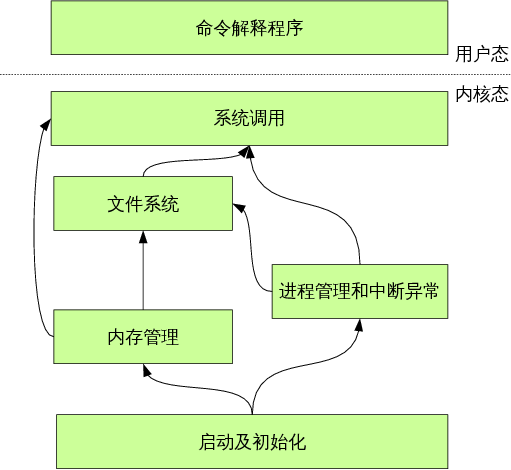
\includegraphics[height=8cm]{7-1}
  \caption{六个实验间的关系}\label{fig:7-1}
\end{figure}

\section{操作系统实验工具}

\subsection{交叉编译器}
首先,整个实验是建立在MIPS上的,通过之前的计算机组成等课程的学习我们知道,不同类型的CPU有不同的ISA。我们本地常使用的是Intel的X86指令集,
或AMD64(EMT64)等指令集。而我们的小操作系统的目标机是MIPS指令集的。但我们需要使用交叉编译器来完成编译过程。
我们的交叉编译器运行于x86平台上,但编译产生的二进制文件却是在mips平台上运行的。如图\ref{fig:0-2}
所示,编译器所运行的平台与其编译出来的程序的平台不同,因此叫做交叉编译器。

\begin{note}
严格意义上来说,所谓平台包含了两个概念:体系结构(Architecture)、操作系统(Operating System)。
一个体系结构上,可以运行多种不同的操作系统。而同一个操作系统,也可以在不同体系结构上运行。
举例来说,我们常说的 x86 Linux 平台实际上是 Intel x86 体系结构和Linux for x86操作系统的统称;
而x86 WinNT平台实际上是Intel x86体系结构和Windows NT for x86 操作系统的简称。
\end{note}

交叉编译器通常用于解决目标平台因性能不足等原因难以直接在其上开发的问题。举个例子,假如我们需要为一个500MHz的ARM开发程序,
因为其性能、工具、环境等原因,我们很难直接在这个ARM的板子上进行开发。因此,我们可以选择在一个性能强劲、工具齐全的x86 PC机上完成程序,
再通过交叉编译器编译为ARM指令集的程序。通过这样的方式,我们就能够轻松地为ARM开发程序了。

\begin{figure}[htbp]
  \centering
  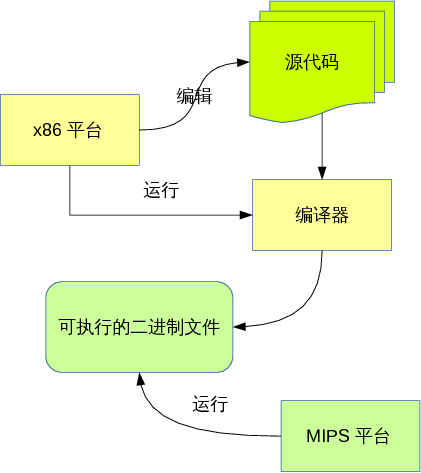
\includegraphics[height=8cm]{7-2}
  \caption{交叉编译}\label{fig:7-2}
\end{figure}

\subsection{Linux系统}
Unix是一个经典的操作系统。目前操作系统中的很多设计思想以及算法均是源自Unix的。
但Unix在商业化后,我们很难以相对廉价的方式直接接触Unix。目前相对较为完善的自由的Unix衍生版仅有FreeBSD等寥寥几个,
其上的软件生态环境等等十分有限。不过,幸运的是,Linux为我们提供了一个相对良好的接触Unix思想的机会。
Linux是一个自由的类Unix(Unix-like)系统,兼容POSIX标准,为我们的实验提供了一个良好的环境。
近些年Linux发展迅猛,其上的软件环境等也十分丰富,这一点相较于BSD家族来说要好很多。
我们实验中采用了GNU的工具,这一套工具主要是为Unix类系统编写的。同时,我们的小操作系统中有很多Unix风格的设计,
因此,采用Linux平台做实验更有利于大家理解实验中的很多内容。实验为大家提供的虚拟机上的环境是一个无图形界面的Ubuntu 12.04,
大家通过ssh远程连接到虚拟机上去做实验。通过命令行界面来进行全部的操作。很多同学以前没有太接触过这种操作方式,这一点需要大家慢慢熟悉。

\begin{note}
事实上,Linux仅仅是一个操作系统内核。一般一个完整的基于Linux的操作系统还包含GNU的各类工具软件,
图形环境,应用软件等等其他一系列的软件。但习惯上,将以Linux为内核的操作系统简称为Linux。
由于大家长期以来习惯在Linux内核上使用大量的GNU软件,所以,Richard Stallman认为将这类操作系统称为“GNU/Linux”更为恰当。
\end{note}

\section{实验环境配置}

\subsection{Linux操作系统}
由于所有的实验都是在Linux下完成的,所以需要Linux操作系统。我们选用设计上更为用户友好的Ubuntu系统。
有两种可供参考的安装方式,一是通过虚拟机来安装Linux系统,二是直接安装Linux系统。这里考虑到大部分同学对于Linux不同熟悉,
我们介绍虚拟机安装的方法。

首先,我们需要下载操作系统的镜像。为了下载速度考虑,我们选择从中国科学与技术大学的镜像站\url{http://mirrors.ustc.edu.cn/}上下载。
点击该页面右侧的\textbf{获取安装镜像},出现如图\ref{fig:get-ubuntu-image}所示的界面,版本选择与实验环境一致的12.04。

\begin{figure}[htbp]
  \centering
  \includegraphics[width=15cm]{get-ubuntu-image}
  \caption{获取安装镜像}\label{fig:get-ubuntu-image}
\end{figure}

接下来,我们下载虚拟机软件。虚拟机相当于一台虚拟的机器,虚拟机上的操作就好像是在操作另一台机器,对本机不会造成影响,
是相对安全的一种体验Linux的方案。这里我们选择采用VirtualBox虚拟机。可以去官网\url{https://www.virtualbox.org/wiki/Downloads}下载,
也可以去百度上自行寻找国内的较快的下载地址。当然,你也可以选择其他的虚拟机软件,如VMware(性能更佳,但是是专有软件,你懂得),具体操作相仿。
但Virtualbox是自由软件,所以出于版权方面的考虑,这里以VirtualBox为例。

安装VirtualBox(相信安装这种小事一定难不住你)后,打开它,看到如图\ref{fig:virtualbox-startup}所示的界面。

\begin{figure}[htbp]
  \centering
  \includegraphics[width=10cm]{virtualbox-startup}
  \caption{VirtualBox虚拟机界面}\label{fig:virtualbox-startup}
\end{figure}

点击\textbf{新建},出现如图\ref{fig:virtualbox-dialog1}所示的对话框。类型选择\textbf{Linux},版本选择\textbf{Ubuntu(64bit)}
(这里如果你下载的时候选择的是i386版本则选择\textbf{Ubuntu(32bit)})。点击\textbf{下一步},内存选择\textbf{1024MB}。
下一步,选择\textbf{现在创建虚拟硬盘},后面的设置如无特殊需求不必改动,一直下一步即可。直到选择磁盘大小处,建议选择\textbf{20GB},
同时选定一个至少有20GB空间的的位置放置磁盘镜像文件。

\begin{figure}[htbp]
  \centering
  \includegraphics[height=8cm]{virtualbox-dialog1}
  \caption{新建虚拟机}\label{fig:virtualbox-dialog1}
\end{figure}

之后选中我们刚才建立的虚拟机,点\textbf{设置},\textbf{存储},点选\textbf{光盘加号形状图标},\textbf{添加虚拟光驱},
如图\ref{fig:virtualbox-dialog2}然后\textbf{选择磁盘},选中之前下载好的Ubuntu的ISO文件。
      
\begin{figure}[htbp]
  \centering
  \includegraphics[width=10cm]{virtualbox-dialog2}
  \caption{选择启动镜像}\label{fig:virtualbox-dialog2}
\end{figure}

选中虚拟机,点击\textbf{启动},弹出虚拟机画面,启动后进入Ubuntu的安装界面(见图\ref{fig:ubuntu-install1})。
左侧可以选择语言,这里我们选择\textbf{English},并点击\textbf{Install Ubuntu}。
(当然,按理说选择中文也是没问题的,但这里为了避免任何不必要的麻烦,我们选择了英文)。

\begin{figure}[htbp]
  \centering
  \includegraphics[width=10cm]{ubuntu-install1}
  \caption{选择启动镜像}\label{fig:ubuntu-install1}
\end{figure}

之后由于我们没有改镜像源等设置,为了安装速度考虑,不要选择\textbf{Download updates while installing}。以免Ubuntu
从缓慢的官方服务器下载更新。\textbf{Install this third-party software}选项与我们实验无关,你可以自行选择是否勾选。
下一步选择\textbf{Erase disk and install Ubuntu}。由于我们是在虚拟机上安装,且使用了新建的虚拟磁盘,所以自然可以大胆
地让Ubuntu清空整个磁盘并安装。下一步一般不需要做改动,点击\textbf{Install Now}就好。之后输入密码,等待安装结束就好。

\begin{figure}[htbp]
  \centering
  \includegraphics[width=10cm]{ubuntu-install2}
  \caption{Ubuntu安装中新建用户的界面}\label{fig:ubuntu-install2} 
\end{figure}

安装结束后点击\textbf{Restart}重启。重启时注意,安装镜像关闭时一般会提示你取出光盘并按回车键。
光盘镜像正常情况下会被自动弹出。
一般来说,你需要做的仅仅是按下回车键并等待重启。
这里注意,有时候由于种种原因它不会输出这句提示,遇到这种情况就需要发动你的第六感了:)感觉系统不再动了以后敲一个回车就好。

重启完成后登入Ubuntu界面,接下来我们安装增强功能。点击虚拟机的\textbf{设备},然后选择\textbf{安装增强功能}。
之后会Ubuntu会选择弹出对话框询问是否自动运行,如图\ref{fig:ubuntu-install3}所示。点击\textbf{Run}后会
弹出对话框要求输入密码,输入密码后会启动一个命令行,开始执行安装脚本,看到\textbf{Press Return to close this window}
后按回车键结束安装。手动重启虚拟机,重启后虚拟机的分辨率会变成相对正常的状态,说明增强功能已经成功安装。

\begin{figure}[htbp]
  \centering
  \includegraphics[width=8cm]{ubuntu-install3}
  \caption{Ubuntu安装中新建用户的界面}\label{fig:ubuntu-install3} 
\end{figure}

至此,一个Ubuntu环境就搭建完成了。你可以在上面学习并熟悉Linux的相关指令,并编写我们的实验代码。

\begin{exercise}
安装一个Linux环境,并尝试学会使用ls、cat、cd、cp、mv这五条指令
\end{exercise}

\subsection{安装交叉编译器}
交叉编译器的下载可以访问\url{http://ftp.sunet.se/pub/Linux/distributions/eldk/4.1/mips-linux-x86/iso/}
到其中下载\textbf{mips-2007-01-21.iso}文件。这里下载网速较慢,建议大家下载完一份后相互拷贝,
一般课程中心也会提供相应的文件。

在Ubuntu下,按住Ctrl+Alt+t快捷键,可以打开一个终端,我们在终端中

\begin{minted}[linenos]{bash}
# 建立一个用于挂载ISO镜像的目录
sudo mkdir /mnt/mipsiso
# 挂载iso文件
sudo mount -o loop mips-2007-01-21.iso /mnt/mipsiso
# 切换到/mnt/mipsiso文件夹中
cd /mnt/mipsiso
# 安装32位运行库(仅在64位系统上需要执行此步骤)
sudo apt-get install ia32-libs
# 运行安装脚本
sudo ./install -d /opt/eldk
\end{minted}

执行完上面的指令后,检查/opt/eldk/usr/bin下是否有以mips\_4KC开头的一系列工具。
打开命令行,尝试运行其中的gcc,如果看到如下输出,则说明一切OK~

\begin{minted}[linenos]{bash}
# 注意,此时需要位于/opt/eldk/usr/bin目录下
$ ./mips_4KC-gcc
Reading specs from /opt/eldk/usr/bin/../lib/gcc/mips-linux/4.0.0/specs
Target: mips-linux
Configured with: /opt/eldk/build/mips-2007-01-21/work/usr/src/denx/
BUILD/crosstool-0.35/build/gcc-4.0.0-glibc-2.3.5-eldk/mips-linux/
gcc-4.0.0/configure --target=mips-linux --host=i686-host_pc-linux-gnu 
--prefix=/var/tmp/eldk.PyrfxY/usr/crosstool/gcc-4.0.0-glibc-2.3.5-eldk
/mips-linux --with-headers=/var/tmp/eldk.PyrfxY/usr/crosstool/gcc-4.0.
0-glibc-2.3.5-eldk/mips-linux/mips-linux/include --with-local-prefix=
/var/tmp/eldk.PyrfxY/usr/crosstool/gcc-4.0.0-glibc-2.3.5-eldk/
mips-linux/mips-linux --disable-nls --enable-threads=posix 
--enable-symvers=gnu --enable-languages=c,c++ --enable-shared 
--enable-c99 --enable-long-long --enable-__cxa_atexit
Thread model: posix
gcc version 4.0.0 (DENX ELDK 4.1 4.0.0)
\end{minted}

\subsection{安装仿真器}
由于实验的操作系统内核是运行在mips体系结构上的,而我们平常使用的是基于x86体系结构的PC,
所以需要使用仿真器来仿真一个mips体系结构的环境,来让我们的操作系统内核运行。在这个实验中我们使用的是 gxemul 仿真器。

我们需要从\url{http://gxemul.sourceforge.net/src/}下载gxemul-0.4.6.tar.gz。
这里需要注意,一定要下载0.4系列的gxemul,而不是最新的0.6系列,以免发生和实验提供的文件发生不兼容的现象。
调出终端,切换到gxemul-0.4.6.tar.gz所在目录,执行以下指令

\begin{minted}[linenos]{bash}
# 解压gxemul-0.4.6.tar.gz
tar -zxvf gxemul-0.4.6.tar.gz
# 进入gxemul文件夹
cd gxemul-0.4.6
# 配置并编译安装
./configure
make
sudo make install
sudo cp gxemul /usr/local/bin
\end{minted}

在命令行中执行gxemul指令,看到如下输出则说明gxemul安装正确。

\begin{minted}[linenos]{bash}
$ gxemul
GXemul 0.4.6    Copyright (C) 2003-2007  Anders Gavare
Read the source code and/or documentation for other Copyright messages.

usage: gxemul [machine, other, and general options] [file [...]]
   or  gxemul [general options] @configfile
   or  gxemul [userland, other, and general options] file [args ...]

Run  gxemul -h  for help on command line options.

No filename given. Aborting.
\end{minted}

\begin{exercise}
安装交叉编译器及gxemul,并确认其正常运行。
\end{exercise}

\section{实验思考}

\begin{thinking}
思考以下几条指令有何作用?
  \begin{itemize}
    \item ls -l
    \item mv test1.c test2.c
    \item cp test1.c test2.c
    \item cd ..
  \end{itemize}
\end{thinking}
我们的整个实验环境全部是运行于Linux基础上的,且所提供的虚拟机是没有安装图形界面的,需要通过ssh远程连接访问。
实验的所有操作全部在命令行下完成。因此,在开始实验前,你需要掌握最基本的一些命令,以保证你可以\textbf{在命令行下生存}

\begin{thinking}
思考grep指令的用法,例如如何查找项目中所有的宏?如何查找指定的函数名?
\end{thinking}
grep指令可以在文件中\textbf{匹配特定的文本}。支持递归匹配(即查找当前目录及子目录下所有文件)、正则表达式等一系列有用的功能。
当你需要在整个项目目录中查找某个函数名、变量名等等的时候,grep将是你手头一个强有力的工具。
这里给一个提示,grep的-a、-i、-r三个选项使用率较高,可以着重了解一下。

\begin{thinking}
思考gcc的-Werror和-Wall两个参数在项目开发中的意义。
\end{thinking}
编译器警告很多时候可以帮你发现一些代码上的错误。善用编译器警告可以大大加快你调试的进度。

\chapter{初识操作系统}

\section{实验目的}
  \begin{enumerate}
    \item 认识操作系统实验环境
    \item 掌握操作系统实验所需的基本工具
  \end{enumerate}
  
在本章中,我们需要去了解实验环境,熟悉Linux 操作系统(Ubuntu),了解控制终端,掌握一些常用工具并能够脱离可视化界面进行工作。本章节难度非常低,旨在让大家熟悉操作系统实验环境的各类工具,为后续实验奠定基础。

\section{初识实验}
所谓工欲善其事必先利其器,我们需要对我们的环境和工具有了足够多的了解才能开始我们的工作,本章内容看似简单,但实则不可忽略,请大家认真对待。
对于课程设计这名称,大家上次接触是《计算机组成课程设计》,也相信这门课程为大家带来了一段难忘而珍贵的记忆。就像“计组”一样,我们的课程也需要如ISE这样的开发环境,但好消息是,我们的环境约束要少得多,那么接下来熟悉一下我们的实验环境。

\subsection{了解实验环境}
实验环境整体配置如下:
\begin{itemize}
    \item 操作系统:Linux虚拟机,Ubuntu
    \item 硬件模拟器:Gxemul
    \item 编译器:GCC
    \item 版本控制:Git
 \end{itemize}
	
Ubuntu操作系统,一款开源的GNU/Linux操作系统,基于Linux内核实现,是目前较为流行的几个Linux发行版之一。GNU (GNU is Not Unix的递归缩写),是一套计划,其中包含了三个协议条款,为我们带来了大量开源软件;Linux:严格意义上指代Linux内核,基于该内核的操作系统众多,具有免费、可靠、安全、稳定、多平台等特点。

GXemul,一款计算机架构仿真器,可以模拟所需硬件环境,例如我们需要的MIPS架构下的CPU。

GCC,一套免费、开源的编译器,诞生并服务于GNU计划,最初名称为GNU C Compiler,后支持了更多编程语言而改名为GNU Compiler Collection,如你所见,简称没变,很多我们熟知的IDE/集成开发环境的编译器用的便是GCC套件,例如Dev-C++,Code::Blocks等。我们的实验将使用mips-C交叉编译器。

Git,一款免费、开源的版本控制系统,我们的实验将用它为大家提供管理、发布、提交、评测等功能。0.5小节将会为大家详细介绍Git为何物以及如何使用,故不在此赘述。

\begin{figure}[htbp]
  \centering
  
\includegraphics[height=4cm]{0-1}
  \caption{Ubuntu,GNU,Linux}\label{fig:0-1}
\end{figure}

\subsection{ssh—远程访问我们的环境}

熟悉了实验环境之后,我们不禁产生了疑问:难道这些环境全部需要我们自行安装和配置?这里为大家带来另一个好消息:当然不是,这些环境已经为你们配置好了!

本实验总计7个Lab完全依赖于远程的数台虚拟机上,最终成果也需要通过这些机器进行提交,所以同学们几乎不用担心个人电脑“带不动”实验环境,你需要的仅仅是一个能够支持ssh协议的远程连接工具。

一般Liunx或Mac OS等类Unix操作系统都会附带ssh客户端,即直接在终端使用ssh命令便可,Windows平台一般不自带ssh,需要下载第三方软件,在这里建议大家使用一款轻量级的,开源的,名为PuTTY的小工具,当然也不乏各种功能强大的工具,接触过git for Windows或对Windows 10有所研究的同学亦可使用git bash的以及Windows 10的几款Linux子系统。

在Host Name部分填入username@ip便可,username为同学们的学号,ip会在课上公布,之后单击open便可

在光标处输入密码便可,密码初始为同学们的学号,因此建议登录后立刻使用passwd命令更改密码,详细操作会在第三节中介绍。

如果同学们是在Mac OS的终端或Linux系统的终端,只需输入 ssh username@ip 之后的操作与PuTTY便相同了。

\begin{minted}[linenos]{bash}
# username 处填写你的用户名,ip处填写远程主机的地址
$ ssh username@ip
# 之后等候片刻会要求你输入密码,输入的密码不会被显示在屏幕上,输入完成后按回车即可
# 链接后会显示一些欢迎信息,下面是欢迎信息的一个例子
Welcome to Ubuntu 12.04.5 LTS (GNU/Linux 3.13.0-32-generic i686)

 * Documentation:  https://help.ubuntu.com/

  System information as of Tue Aug 11 09:55:40 CST 2015
  System load:  0.0                Processes:           118
  Usage of /:   8.7% of 145.55GB   Users logged in:     0
  Memory usage: 6%                 IP address for eth0: 0.0.0.0
  Swap usage:   0%

  Graph this data and manage this system at:
    https://landscape.canonical.com/

0 packages can be updated.
0 updates are security updates.
# 欢迎信息后会出现命令提示符,等待你输入命令。
\end{minted}

\begin{figure}[htbp]
  \centering
  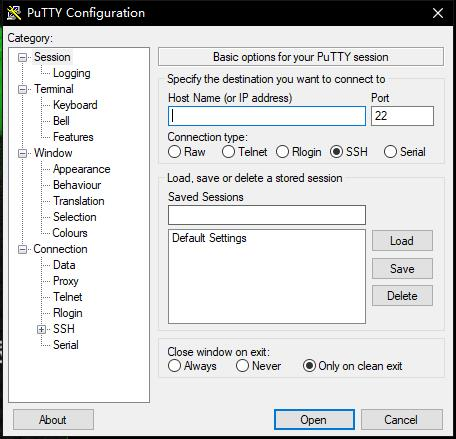
\includegraphics[height=8cm]{0-2}
  \caption{PuTTY登录界面}\label{fig:0-2}
\end{figure}

\begin{note}
SSH是Secure Shell的缩写。它是一种用于建立安全的远程连接的网络协议。在Unix类系统上被广泛采用。
除了连接到远程网络,目前SSH还有一种较为有趣的用法。当你既想用Windows,又有时需要Unix环境时,
可以利用Windows8及以上版本自带的Hyper-V开启一个Linux虚拟机(不必开启图形界面)。
之后通过SSH客户端连接到本机上的Linux虚拟机上,即可获得一个Unix环境。甚至可以开启X11转发,
即可在Windows上开启一些Linux上的带图形界面的程序,十分方便。
\end{note}

\subsection{接触CLI Shell,告别GUI Shell}

当你使用如上方法登录了自己的账号后,可能会有点不知所措并产生疑问:在我面前的这些东西是什么?

简单来说,这就是你们要接触的操作系统Ubuntu,在这里为从未使用过命令行的同学们解释一下,当你阅读这份文档时,你所使用的一定是一款拥有图形化界面的操作系统,一般来讲是Windows、Mac OS、Ubuntu等,而你面前的这个黑黑的东西就是一个没有图形化界面的操作系统,也就是模拟终端,我们为什么剥夺了你使用图形化界面的权力呢,原因有二:1.为了锻炼同学们在相对图形化恶劣的环境下工作的能力;2.你们的任务通过终端全部可以实现。

当然上文的描述是不严谨的,你所面对的并不是真正的“Ubuntu操作系统”,而是它的“壳”。一般的,我们管操作系统核心部分称为内核(英文:Kernel),与其相对的就是它最外层的壳(英文:Shell)。Shell是用于访问操作系统服务的用户界面。一般而言,操作系统shell使用命令行界面(CLI)或图形用户界面(GUI),这个纯文本的界面就是命令行界面,它能接收你发送的命令,如果命令存在于环境中,它便会为你提供相应的功能。

在Ubuntu中,我们默认使用的CLI shell是bash,也是一款基于GNU的免费、开源软件,那么接下来我们小试牛刀。

\begin{exercise}
在bash中分别输入
  \begin{itemize}
    \item echo “Hello Ubuntu”
    \item bash --version
    \item ls
  \end{itemize}
三条命令,简单思考其回显结果
\end{exercise}

可以保证的是,当你掌握了本章的知识后,再使用这款未为你准备图形化界面的操作系统时,将会得心应手,相信你能发挥出它本真的功能。

\begin{thinking}\label{think-Shell简析}
通过你的使用经验,简单分析CLI Shell,GUI Shell在你使用过程中的各自优劣(100字以内)
\end{thinking}

\subsection{获取实验包}

当我们登陆了课程实验环境后,就要准备开始我们的实验了,好奇的你可能会问:环境有了,工具有了,我们在哪里完成实验呢?

我们在ip服务器上为所有同学部署了实验的远程仓库,接下来我们要先进行一条命令来获取我们的实验包。
\begin{minted}[linenos]{bash}
$ git clone git@ip:id-lab
\end{minted}
接下来系统会提示如下内容
\begin{minted}[linenos]{bash}
Cloning into '16xxxxxx-lab'...
Enter passphrase for key '/home/16xxxxxx/.ssh/id_rsa':
\end{minted}
这里让你输入你的rsa密钥,也就是每个人的学号。

执行之后若输入ls,你会发现你的主目录下多了一个id-lab,输入如下命令访问它
\begin{minted}[linenos]{bash}
$ cd id-lab
\end{minted}
再使用ls会发现里面空空如也,不用着急,接下来需要再执行一条命令
\begin{minted}[linenos]{bash}
$ git checkout lab0
\end{minted}
这样我们就进入Lab0工作区了,也许你现在对上面的几条命令的功能不太了解,没关系,本章的后续内容会为你介绍它们。

\section{基础操作介绍}
\subsection{命令行}
走到这里,我们要正式与那黑黑的界面交流了,命令行界面(Command Line Interface,简称CLI)中,用户或客户端通过单条或连续命令行的形式向程序发出命令,从而达到与计算机程序进行人机交互的目的。在Linux系统中,命令即是对Linux系统进行管理的一系列命令,其一般格式为:命令名 [选项] [参数],其中中括号表示可选,意为可有可无(例如: ls –a directory)。对于Linux系统来说,无论是中央处理器、内存、磁盘驱动器、键盘、鼠标,还是用户等都是文件,Linux系统的管理命令是它正常运行的核心,与Windows的命令提示符(CMD)命令类似。Linux命令在系统中有两种类型:内置Shell(外壳)命令和Linux命令。

对于刚接触到命令行界面的各位萌新们来说,因为不清楚基本的Linux命令而呆呆地望着屏幕上的光标,想要做些什么却又不知所措是再正常不过的事。不过不要着急,万事开头难,学会并可以熟练使用下面介绍的一些基本操作之后,相信你们一定会对命令行界面有一个全新的认识,不再一头雾水。

\subsection{Linux基本操作命令}
通过SSH连接服务器打开Linux命令行界面后,首先会看到光标前的如下内容,其中@符号前的是用户名,@符号后的是计算机名,冒号后为当前所在的文件目录(/表示根目录root;~表示主目录home,其一般等价于/home/<user\_name>),最后的\$或\#分别表示当前用户为普通用户或超级用户root,当然,我们的服务器自然不会让大家知道root的密码的,感兴趣的同学可以自己配置系统娱乐一番

\begin{minted}[linenos]{bash}
16xxxxxx@ubuntu:~$
\end{minted}
\begin{minted}[linenos]{bash}
root@ubuntu:~#
\end{minted}

现在通过键盘输入命令,按回车后即可执行。首先,我们需要更改自己的用户密码,使用passwd命令即可更改当前用户的密码,注意:输入密码时不会在屏幕上显示密码内容(若输入过程中手抖打错,可重复多按几次退格键清空之前的输入后重新输入)。

\begin{minted}[linenos]{bash}
16xxxxxx@ubuntu:~$ passwd
更改16xxxxxx的密码。
(当前)UNIX密码:
输入新的UNIX密码:
重新输入新的UNIX密码:
passwd:已成功更新密码
\end{minted}

更改完密码后我们就可以安全的使用此用户来完成工作了,面对一个全新的界面,我们首先要知道当前目录中都有哪些文件,这时就需要使用ls命令,其输出信息可以进行彩色加亮显示,以分区不同类型的文件,是使用率较高的命令,其详细信息如下图所示。一般情况下,该命令的参数省略则默认显示该目录下所有文件,所以我们只需使用ls即可看到所有非隐藏文件,若要看到隐藏文件则需要加上-a选项,若要查看文件的详细信息则需要加上-l选项。

\begin{minted}[linenos]{bash}
ls - list directory contents
用法:ls [选项]... [文件]...
选项(常用):
		-a		不隐藏任何以. 开始的项目
		-l		每行只列出一个文件
\end{minted}

\begin{note}
与ls命令类似的目录查看命令还有tree命令,它可以根据文件目录生成文件树,这个命令就交给大家自己去实践吧。
\end{note}

然后你就会发现主目录中空空如也,又不知道要做什么好了,这时我们可以使用mkdir命令创建文件目录(即Windows系统中的文件夹),该命令的参数为创建的新目录的名称,如:mkdir newdir 为创建一个名为newdir的目录。

\begin{minted}[linenos]{bash}
mkdir - make directories
用法:mkdir [选项]... 目录...
\end{minted}

删除空目录的命令rmdir与其类似,其命令参数为需要删除的空目录的名称,这里要注意只有空目录才可以使用rmdir命令删除。

\begin{minted}[linenos]{bash}
rmdir - remove empty directories
用法:rmdir [选项]... 目录...
\end{minted}

那么目录非空时怎么办呢?这就需要用到搞破坏者最喜欢的rm命令了,rm命令可以删除一个目录中的一个或多个文件或目录,也可以将某个目录及其下属的所有文件及其子目录均删除掉。对于链接文件,只是删除整个链接文件,而原有文件保持不变。

\begin{minted}[linenos]{bash}
rm - remove files or directories
用法:rm [选项]... 文件...
选项(常用):
		-r		递归删除目录及其内容
		-f		强制删除。忽略不存在的文件,不提示确认
\end{minted}

\begin{note}
使用rm命令要格外小心,因为一旦删除了一个文件,就无法再恢复它。所以,在删除文件之前,最好再看一下文件的内容,确定是否真要删除。
\end{note}

此外,rm命令可以用-i选项,这个选项在使用文件扩展名字符删除多个文件时特别有用。使用这个选项,系统会要求你逐一确定是否要删除。这时,必须输入y并按Enter键,才能删除文件。如果仅按Enter键或其他字符,文件不会被删除。与之相对应的就是-f选项,强制删除文件或目录,不询问用户。使用该选项配合-r选项,进行递归强制删除,强制将指定目录下的所有文件与子目录一并删除可以达到毁灭性效果。例如:rm –rf / 即可强制递归删除全盘文件,有兴趣的同学可以尝试一下,反正你们也没有这个权限~

\begin{note}
在需要键入文件名/目录名时,可以使用TAB键补足全名,当有多种补足可能时双击TAB键可以显示所有可能选项。
\end{note}

学会创建目录后,我们就需要进入我们新建的目录中创建和修改文件来完成工作了。使用cd命令来切换工作目录至dirname,其中dirname的表示法可为绝对路径或相对路径。若目录名称省略,则变换至使用者的主目录home (等价于cd ~ )。另外,在Linux文件系统中,"."表示当前所在目录,".."表示当前目录位置的上一层目录,同学们在使用ls –a后看到的目录中的"."和".."即使如此。

\begin{minted}[linenos]{bash}
cd - change working directory
用法:cd [路径]
e.g.
		cd .	变更至当前目录
		cd ..	变更至父目录
\end{minted}

现在,进入新建的目录中后依旧空空如也,那么我们就来创建几个文件玩玩~创建文件的方法有很多,可以直接使用重定向输出>filename来新建一个空文件,也可以使用文本编辑工具vim或nano等新建文件后保存(使用命令vim filename或nano filename,编辑工具的使用方法将在0.4节介绍),因为打开后可以直接进行编辑后保存,所以笔者更喜欢用后者新建文件。现在可能有人要问了,重定向输出是什么意思?大于号是什么意思?重定向输出就是使用>来改变送出的数据信道,使>前命令的输出数据输出到>后指定的文件中去。例如:ls / > filename 可以将根目录下的文件名输出至当前目录下的filename文件中。与之类似的,还有重定向追加输出>>,将>>前命令的输出数据追加输出到>>后指定的文件中去;以及重定向输入<,将<后指定的文件中的数据输入到<前的命令中,同学们可以自己动手实践一下。

在此顺带一提echo命令,echo命令用于在Shell中打印Shell变量的值,或者直接输出指定的字符串。简单来说,就是将echo命令中的参数输出到屏幕上显示。那么将echo命令和重定向相结合会产生什么样的效果呢?这就留给大家自己去尝试吧~

好了,现在我们已经创建了新的文件,那么想要查看文件内容要怎么办呢?除了前面说到的编辑工具以外,还有一种简单快速查看文件内容的方法——cat命令。使用cat filename即可将文件内容输出到屏幕上显示,若要显示行数,添加-n选项即可。

\begin{minted}[linenos]{bash}
cat - concatenate files and print
用法:cat [选项]... [文件]...
选项(常用):
		-n		对输出的所有行编号
\end{minted}

\begin{exercise}
	执行如下命令,并查看结果
	\begin{itemize}
		\item echo first
		\item echo second > output.txt
		\item echo third > output.txt
		\item echo forth >> output.txt
	\end{itemize}
\end{exercise}
之后就是对于文件的操作:复制和移动。复制命令为cp,命令的第一个参数为源文件路径,命令的第二个参数为目标文件路径。

\begin{minted}[linenos]{bash}
cp - copy files and directories
用法:cp [选项]... 源文件... 目录
选项(常用):
		-r		递归复制目录及其子目录内的所有内容
\end{minted}

移动命令为mv,与cp的操作相似。例如:mv file ../file\_mv就是将当前目录中的file文件移动至上一层目录中且重命名为file\_mv。聪明的你应该已经看出来,在Linux系统中想要对文件进行重命名操作,使用mv oldname newname命令就可以了。
\begin{minted}[linenos]{bash}
mv - move/rename file
用法:mv [选项]... 源文件... 目录
\end{minted}

在以后的工作中,可能会遇到重复多次用到单条或多条长而复杂命令的情况,初学者可能会想把这些命令保存在一个文件中,以后再打开文件复制粘贴运行,其实大可不必复制粘贴,将文件按照批处理脚本运行即可。简单来说,批处理脚本就是存储了一条或多条命令的文本文件,Linux系统中有一种简单快速执行批处理文件的方法(类似Windows系统中的.bat批处理脚本)——source命令。source命令是bash的内置命令,该命令通常用点命令 . 来替代。这两个命令都以一个脚本为参数,该脚本将作为当前Shell的环境执行,不会启动一个新的子进程,所有在脚本中设置的变量将成为当前Shell的一部分。使用方法如下图所示,其命令格式与之前介绍的命令类似,请同学们自己动手举例尝试。

\begin{minted}[linenos]{bash}
source - execute commands in file
用法:source 文件名 [参数]
注:文件应为可执行文件,即为绿色
\end{minted}

\begin{thinking}\label{think-文件的操作}
使用你知道的方法(包括重定向)创建下图内容的文件(文件命名为test),将创建该文件的命令序列保存在command文件中,并将test文件作为批处理文件运行,将运行结果输出至result文件中。给出command文件和result文件的内容,并对最后的结果进行解释说明(可以从test文件的内容入手)
\end{thinking}
\begin{figure}[htbp]
	\centering
	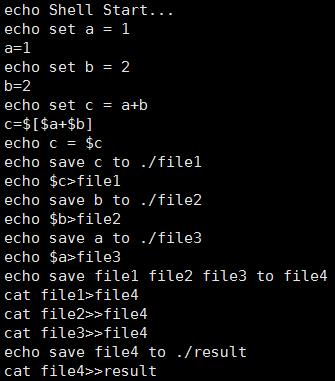
\includegraphics[height=8cm]{0-15}
	\caption{文件内容}\label{fig:0-15}
\end{figure}

此外,还有两种常用的查找命令:find和grep

使用find命令并加上-name选项可以在当前目录下递归地查找符合参数所示文件名的文件,并将文件的路径输出至屏幕上。

\begin{minted}[linenos]{bash}
find - search for files in a directory hierarchy
用法:find -name 文件名
\end{minted}

grep是一种强大的文本搜索工具,它能使用正则表达式搜索文本,并把匹配的行打印出来。简单来说,grep命令可以从文件中查找包含pattern部分字符串的行,并将该文件的路径和该行输出至屏幕。当你需要在整个项目目录中查找某个函数名、变量名等特定文本的时候,grep 将是你手头一个强有力的工具。

\begin{minted}[linenos]{bash}
grep - print lines matching a pattern
用法:grep [选项]... PATTERN [FILE]...
选项(常用):
		-a		不忽略二进制数据进行搜索
		-i		忽略文件大小写差异
		-r		从文件夹递归查找
\end{minted}

以上,就是Linux系统入门级的部分常用操作命令以及这些命令的常用选项,如果想要查看这些命令的其他功能选项或者新命令的详尽说明,就需要使用Linux下的帮助命令——man命令,通过man指令可以查看Linux中的指令帮助、配置文件帮助和编程帮助等信息。

\begin{minted}[linenos]{bash}
man - manual
用法:man page
e.g.
	man ls
\end{minted}

最后,还有下面几个常用的快捷键介绍给同学们。
\begin{itemize}
    \item Ctrl+C	终止当前程序的执行
	\item Ctrl+Z	挂起当前程序
	\item Ctrl+D	终止输入(若正在使用Shell,则退出当前Shell)
	\item Ctrl+I	清屏
\end{itemize}

其中,Ctrl+Z挂起程序后会显示该程序挂起编号,若想要恢复该程序可以使用fg <编号>即可。对其他内容感兴趣的同学可以自行百度或用man命令看帮助手册进行学习和了解。

\begin{note}
在多数shell中,四个方向键也是有各自特定的功能的:←和→可以控制光标的位置,↑和↓可以切换最近使用过的命令
\end{note}

\section{实用工具介绍}
学会了Linux基本操作命令,我们就可以得心应手地使用命令行界面的Linux操作系统了,但是想要使用Linux系统完成工作,光靠命令行还远远不够。在开始动手阅读并修改代码之前,我们还需要掌握一些实用工具的使用方法。这里我们首先介绍两种常用的文本编辑器:nano和Vim。
\subsection{nano}
我们先从一个简易的工具入手:nano。nano的主界面如下图所示,所有基本的操作都被罗列在下面。nano 较为容易上手,但功能相对有限。如果你需要更为强大的功能,那么推荐去学习和使用Vim。

\begin{figure}[htbp]
  \centering
  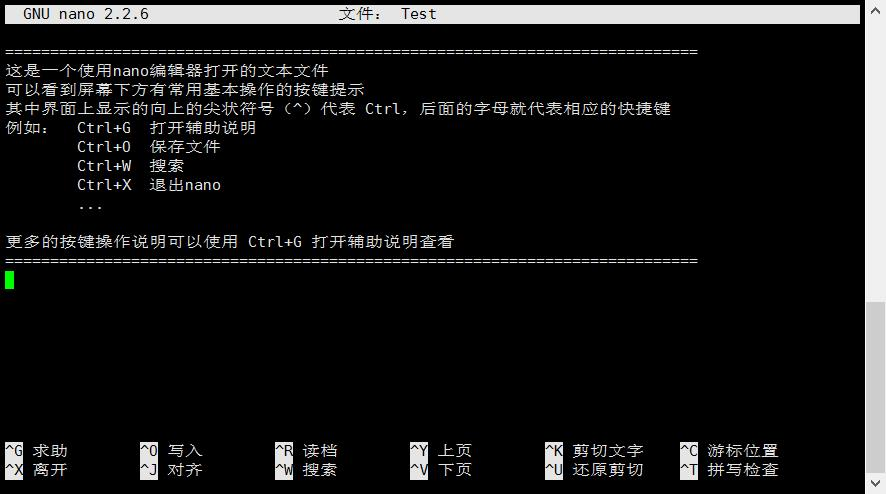
\includegraphics[height=8.5cm]{0-20}
  \caption{Nano界面及基础介绍}\label{fig:0-20}
\end{figure}

\subsection{Vim}
Vim被誉为编辑器之神,是程序员为程序员设计的编辑器,编辑效率高,十分适合编辑代码,其界面如下图\ref{fig:0-21}所示。对于习惯了图形化界面文本编辑软件的同学们来说,刚接触Vim时一定会觉得非常不习惯非常不顺手,所以在这里给大家总结了一些常用的基本操作以助入门。同时,推荐给大家一篇质量极高的Vim教程——《简明Vim练级攻略》(\url{http://coolshell.cn/articles/5426.html/}),只需要十多分钟的阅读,你就可以掌握 Vim的所有基本操作。当然,想要完全掌握它需要相当长的时间去练习,而如果你只想把Vim当成记事本用的话,几分钟的学习足矣。其他的内容网上有太多太多的资料,随用随查即可。

\begin{figure}[htbp]
  \centering
  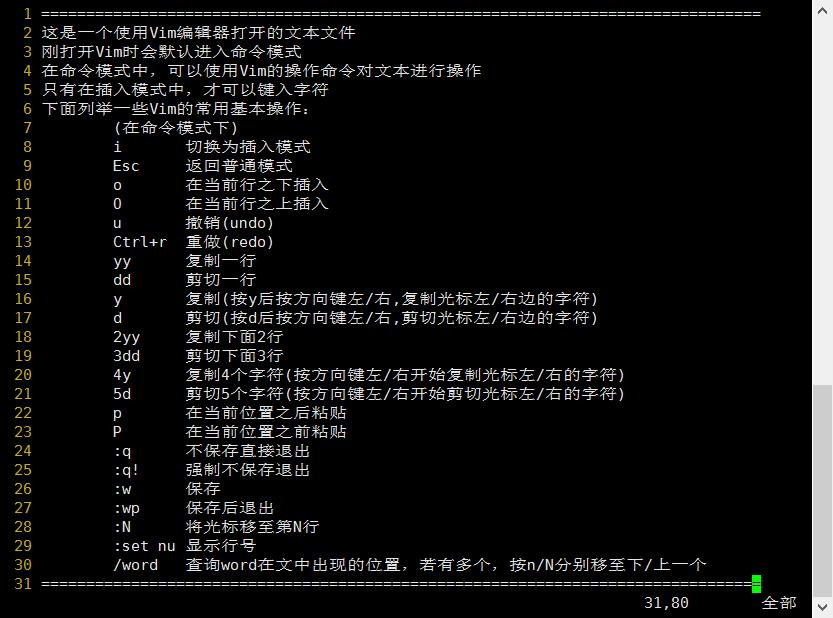
\includegraphics[height=11cm]{0-21}
  \caption{Vim界面及基础介绍}\label{fig:0-21}
\end{figure}

\subsection{GCC}
在没有IDE的情况下,使用GCC编译器是一种简单快捷生成可执行文件的途径,只需一行命令即可将C源文件编译成可执行文件。其常用的使用方法如下图\ref{fig:0-22}所示,同学们可以自己动手实践,写一些简单的C代码来编译运行。如果想要同时编译多个文件,可以直接用-o选项将多个文件进行编译连接:gcc testfun.c test.c -o test ,也可以先使用-c选项将每个文件单独编译成.o文件,再用-o选项将多个.o文件进行连接:gcc -c testfun.c -> gcc -c test.c -> gcc testfun.o test.o -o test ,两者等价。

\begin{minted}[linenos]{bash}
语法:gcc [选项]... [参数]...
选项(常用):
		-o		指定生成的输出文件
		-S		将C代码转换为汇编代码
		-wall	显示警告信息
		-c		仅执行编译操作,不进行链接操作
		-M		列出依赖
参数:
	C源文件:指定C语言源代码文件
e.g.

$ gcc test.c
#默认生成名为a.out的可执行文件
#Windows平台为a.exe

$ gcc test.c -o test
#使用-o选项生成名为test的可执行文件
#Windows平台为test.exe
\end{minted}

\section{Git专栏--轻松维护和提交代码}
经过上面的一系列的学习之后,你刚刚伸了个懒腰,也许准备喝杯茶休息休息。但突然你意识到了一个问题:之前好像说,有一个叫做Git的东西能对我们的学习进行评测?我们的实验是通过git版本控制系统进行管理,那么接下来,在本章的最后,我们就来了解一下git相关的内容。
\subsection{Git是什么?}
说到Git是什么,我们就得考虑什么是版本控制,最原始的版本控制是纯手工的版本控制:修改文件,保存文件副本。有时候偷懒省事,保存副本时命名比较随意,时间长了就不知道哪个是新的,哪个是老的了,即使知道新旧,可能也不知道每个版本是什么内容,相对上一版作了什么修改了,当几个版本过去后,很可能就是下面的样子了:
\begin{figure}[htbp]
  \centering
  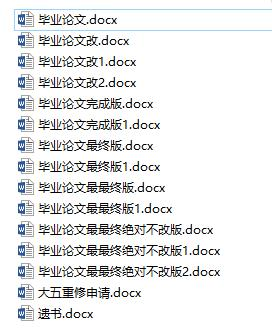
\includegraphics[height=6cm]{0-23}
  \caption{手工版本控制}\label{fig:0-23}
\end{figure}

当然,有些时候,我们不仅是一个人写文本,那些工程项目也往往不是由一个人负责。

分工,制定计划,埋头苦干,看起来一切井然有序,后来却只会让人蛋疼不已。本质原因在于每个人都会对项目的内容进行改动,结果最后有了这样一副情形:A把添加完功能的项目打包发给了B,然后自己继续添加功能。一天后,B把他修改后的项目包又发给了A,这时A就必须非常清楚发给B之后到他发回来的这段期间,自己究竟对哪里做了改动,然后还要进行合并,相当困难。

这时我们发现了一个无法避免的事实:如果每一次小小的改动,项目负责人之间都要相互通知,那么一些错误的改动将会令我们付出惨痛的代价:一个错误的改动要频繁在几方同时通知纠正。如果一次性改动了大幅度的内容,那么只有概览了项目的多数文件才能知道改动在哪,也才能合并劳动成果。项目只有10个文件时还好接受,如果是40个, 60个,80个呢。

于是就产生了需求,我们希望有一款软件:
\begin{itemize}
    \item 自动帮我记录每次文件的改动,而且最好是有后悔药的功能,改错了一个东西,我可以轻松撤销。
	\item 还得有多人协作编辑不费力的好处,有着简洁的指令与操作。
	\item 最好能像时光机一样穿越回以前,而且不但能穿越回去,还能在不满意的时候穿越回来!
	\item 如果想查看某次改动,只需要在软件里瞄一眼就可以。
\end{itemize}
那岂不是美滋滋~

版本控制系统就是这样一种神器的系统。而 Git,则是目前世界上最先进的分布式版本控制系统,没有之一。

Git是由Linux的缔造者Linus Torvalds创造,最开始也是用于管理自己的Linux开发过程。他对于Git的解释是:The stupid content tracker,傻瓜内容追踪器。Git一次本身也是个俚语,大概表示“混帐”。

\begin{note}
版本控制是一种记录若干文件内容变化, 以便将来查阅特定版本修订情况的系统。
\end{note}

\subsection{Git基础指引}
看过上面的小案例后,相信好奇心旺盛的各位已经对Git充满了兴趣。那么Git在实际应用中究竟是怎样的一个系统呢?别着急,我们慢慢来。

先从Git最基础的指令讲起,通过前几节的学习,接下来请进行如下操作:
\begin{enumerate}
    \item 创建一个名为learnGit的文件夹
    \item 进入learnGit目录
	\item 输入git init
	\item 用ls指令添加适当参数看看多了什么
\end{enumerate}
我们会发现,新建的目录下面多了一个叫.git的隐藏目录,这个目录就是我们的Git版本库,更多的被称为仓库(repository)。需要注意的是,\textbf{在我们的实验中是不会对.git文件夹进行任何直接操作的,所以不要轻易动这个文件夹中的任何文件}

在init执行完后,我们就拥有了一个仓库。我们建立的learnGit文件夹就是Git里的工作区。目前我们除了.git版本库目录以外空无一物。

\begin{note}
在我们的小操作系统实验中我们不需要使用到 git init 命令,每个人一开始就都有一个名为 16xxxxxx-lab 的版本库,包含了 lab0 的实验内容。
\end{note}
既然工作区里空荡荡的,那我们来为他加点料:
用你已知的方法在工作区中建立一个readme.txt,内容为“BUAA\_OSLAB”
当然这只是创建了一个文件而已,下面我们要将它添加至版本库,执行如下内容
\begin{minted}[linenos]{bash}
$ git add readme.txt
\end{minted}
注意,到这里还没有结束,你可能会想,那我既然都把 readme.txt 加入了,难道不是已经提交到版本库了吗?但事实就是这样,Git——同其他大多数版本控制系统一样,add之后需要再执行一次提交操作,提交操作的命令如下:
\begin{minted}[linenos]{bash}
$ git commit
\end{minted}
如果不带任何附加选修,执行后会弹出一个说明窗口,如下所示:
\begin{minted}[linenos]{bash}
GNU nano 2.2.6    文件: /home/13061193/13061193-lab/.git/COMMIT_EDITMSG              

Notes to test.
# 请为您的变更输入提交说明。以 '#' 开始的行将被忽略,而一个空的提交
# 说明将会终止提交。
# 位于分支 master
# 您的分支与上游分支 'origin/master' 一致。
#
# 要提交的变更:
#       修改:         readme.txt
#

                                 [ 已读取9 行 ]
^G 求助      ^O 写入      ^R 读档      ^Y 上页      ^K 剪切文字  ^C 游标位置
^X 离开      ^J 对齐      ^W 搜索      ^V 下页      ^U 还原剪切  ^T 拼写检查
\end{minted}
在上面里书写的 \textbf{Notes to test}. 是我们本次提交所附加的说明。

注意,弹出的窗口中我们\textbf{必须}得添加本次 commit 的说明,这意味着我们不能提交空白说明,否则我们的提交不会成功。而且在添加评论之后,可以按提示按键来成功保存。

\begin{note}
初学者一般不太重视 git commit 内容的有效性,总是使用无意义的字符串作为说明提交。但以后你可能就会发现自己写了一个自己看得懂,别人也能看得懂提交说明是多么庆幸。所以尽量让你的每次提交显得有意义,比如“fixedabug in ...” 这样的描述,顺便推荐一条命令:git commit --amend,这条命令可以重新书写你最后一次 commit 的说明。
\end{note}

可能这样的窗口提交方式比较繁琐,我们可以采用一种简洁的方式:
\begin{minted}[linenos]{bash}
$ git commit -m [comments]
\end{minted}
[comments]格式为\textbf{“评论内容”},上述的提交过程我们可以简化为下面一条指令
\begin{minted}[linenos]{bash}
$ git commit -m "Notes to test."
\end{minted}
如果我们提交之后看到类似的提示就说明我们提交成功了
\begin{minted}[linenos]{bash}
[master 955db52] Notes to test.
 1 file changed, 1 insertion(+), 1 deletion(-)
\end{minted}
从我们本次提交中我们可以得到以下信息,可能现在你还不能完全理解这些信息代表的意思,但是没关系,之后我们会讲解

\begin{itemize}
\item 本次提交的分支\label{分支}是 master
\item 本次提交的ID是 955db52
\item 提交说明是 Notes to test
\item 共有1个文件相比之前发生了变化:1行的添加与1行的删除行为
\end{itemize}

但是在我们实验中,第一次提交可不会这么一帆风顺,我们第一次提交往往会出现 下面的提示
\begin{minted}[linenos]{c}
*** Please tell me who you are.

Run

  git config --global user.email "you@example.com"
  git config --global user.name "Your Name"

# to set your account’s default identity.
# Omit --global to set the identity only in this repository.
\end{minted}

相信大家从第一句也能推测出,这是要求我们设置提交者身份的。我们设置身份有 什么作用呢?别急,等你设置成功了我们再详谈。

\begin{note}
从上面我们也知道了,我们可以用  

  git config -{}-global user.email “you@example.com”
  
  git config -{}-global user.name “Your Name“
  
这两条命令设置我们的名字和邮箱,在我们的实验中对这两个没有什么要求,大家随性设置就好,给个示例:

  git config -{}-global user.email “qianlxc@126.com”
  
  git config -{}-global user.name “Qian”
\end{note}

现在你已设置了提交者的信息,那么做一下这个小练习来快速上手 Git 的使用吧。

\begin{exercise}
\begin{itemize}
    \item 在/home/16xxxxxx/learnGit(已init)目录下创建一个名为README.txt的文件。这时使用 git status > Untracked.txt 。
	\item 在 README.txt 文件中随便写点什么,然后使用刚刚学到的 add 命令,再使用 git status > Stage.txt 。
	\item 之后使用上面学到的 Git 提交有关的知识把 README.txt 提交,并在提交说明里写入自己的学号。
	\item 使用 cat Untracked.txt 和 cat Stage.txt,对比一下两次的结果,体会一下README.txt 两次所处位置的不同。
	\item 修改 README.txt 文件,再使用 git status > Modified.txt 。
	\item 使用 cat Modified.txt ,观察它和第一次 add 之前的 status 一样吗,思考一 下为什么?
\end{itemize}
\end{exercise}

\begin{note}
git status 是一个查看当前文件状态的有效指令,而 git log 则是提交日志,每commit一次,Git 会在提交日志中记录一次。git log 将在我们后面乘坐时光机时发挥很大的作用。
\end{note}

相信你做过上述实验后,心里还是会有些疑惑,没关系,我们来一起看一下我们刚才得到的 Untracked.txt ,Stage.txt 和 Modified.txt 的内容
\begin{minted}[linenos]{bash}
Untracked.txt的内容如下

# On branch master
# Untracked files:
#   (use "git add <file>..." to include in what will be committed)
#
#	README.txt
nothing added to commit but untracked files present (use "git add" to track)

Stage.txt的内容如下

# On branch master
# Changes to be committed:
#   (use "git reset HEAD <file>..." to unstage)
#
#	new file:   README.txt
#

Modified.txt的内容如下

# On branch master
# Changes not staged for commit:
#   (use "git add <file>..." to update what will be committed)
#   (use "git checkout -- <file>..." to discard changes in working directory)
#
#	modified:   README.txt
#
no changes added to commit (use "git add" and/or "git commit -a")
\end{minted}
通过仔细观察,我们看到第一个文本文件中第 2 行是:Untracked files,而第二个文本文件中第二行内容是:Changes to be committed,而第三个则是 Changes not staged for commit。这三种不同的提示意味着什么,需要你通过后面的学习找到答案,答案就在不远处。

我们开始时已经介绍了 Git 中的工作区的概念,接下来的内容就是 Git 中的最核心的概念,为了能自如运用 Git 中的命令,你一定要仔细学习。

\subsection{Git文件状态}
首先对于任何一个文件, 在 Git 内都只有四种状态: 未跟踪 (untracked)、未修改 (unmodified)、已修改 (modified)、已暂存 (staged)
\begin{description}
\item[未跟踪] 表示没有跟踪(add)某个文件的变化,使用git add即可跟踪文件
\item[未修改] 表示某文件在跟踪后一直没有改动过或者改动已经被提交
\item[已修改] 表示修改了某个文件,但还没有加入(add)到暂存区中
\item[已暂存] 表示把已修改的文件放在下次提交(commit)时要保存的清单中
\end{description}

\begin{note}
关于刚才的 exercise 中的思考,实际上是因为 git add 指令本身是有多义性的,虽然差别较小但是不同情境下使用依然是有区别。我们现在只需要记住:新建文件后要 git add,修改文件后也需要 git add。
\end{note}

我们使用一张图来说明文件的四种状态的转换关系

\begin{figure}[htbp]
	\centering
	\includegraphics[width=9.5cm]{git-change}
	\caption{Git中的四种状态转换关系}\label{fig:git-change}
\end{figure}

\begin{thinking}\label{think-箭头与指令}
仔细看看这张图,思考一下红箭头里的 add the file 、stage the file 和commit 分别对应的是 Git 里的哪些命令呢?
\end{thinking}

看到这里,相信你对 Git 的设计有了初步的认识。下一步我们就来深入理解一下 Git 里的一些机制,从而让我们可以一次上手,终身难忘。

\subsection{Git三棵树}
我们的本地仓库由 git 维护的三棵“树”组成。第一个是我们的工作区,它持有实际文件;第二个是暂存区(Index 有时也称 Stage),它像个暂时存放的区域,临时保存你的改动;最后是 HEAD,指向你最近一次提交后的结果。 

在我们的.git 目录中,文件.git/index 实际上就是一个包含文件索引的目录树,像是一个虚拟的工作区。在这个虚拟工作区的目录树中,记录了文件名、文件的状态信息(时间戳、文件长度等),但是文件的内容并不存储其中,而是保存在 Git 对象库(.git/objects)中,文件索引建立了文件和对象库中对象实体之间的对应。下面这个图展示了工作区、版本库中的暂存区和版本库之间的关系,希望你能耐着性子仔细理解这张图和不同操作所带来的不同影响。

\begin{figure}[htbp]
  \centering
  \includegraphics[width=15cm]{git-stage}
  \caption{工作区、暂存区和版本库}\label{fig:git-stage} 
\end{figure}

\begin{itemize}
\item 图中 objects 标识的区域为 Git 的对象库,实际位于 ".git/objects" 目录下。
\item 图中左侧为工作区,右侧为版本库。在版本库中标记为 "index" 的区域是暂存区(stage, index),标记为 "master" 的是 master 分支所代表的目录树。
\item 图中我们可以看出此时 "HEAD" 实际是指向 master 分支的一个“游标”。所以图示的命令中出现 HEAD 的地方可以用 master 来替换。
\item 当对工作区修改(或新增)的文件执行 "git add" 命令时,暂存区的目录树被更新,同时工作区修改(或新增)的文件内容被写入到对象库中的一个新的对象中,而该对象的ID 被记录在暂存区的文件索引中。
\item 当执行提交操作(git commit)时,会将暂存区的目录树写到版本库(对象库)中,master 分支会做相应的更新。即 master 指向的目录树就是提交时暂存区的目录树。
\item 当执行 "git rm -{}-cached <file>" 命令时,会直接从暂存区删除文件,工作区则不做出改变。
\item 当执行 "git reset HEAD" 命令时,暂存区的目录树会被重写,被 master 分支指向的目录树所替换,但是工作区不受影响。
\item 当执行 "git checkout -{}- <file>" 命令时,会用暂存区指定的文件替换工作区的文件。这个操作很危险,会清除工作区中未添加到暂存区的改动。
\item 当执行 "git checkout HEAD <file>" 命令时,会用 HEAD 指向的 master 分支中的指定文件替换暂存区和以及工作区中的文件。这个命令也是极具危险性的,因为不但会清除工作区中未提交的改动,也会清除暂存区中未提交的改动。
\end{itemize}

我们在下载软件的时候常常会我们在考虑暂存区和版本库的关系的时候,可以粗略 地认为暂存区是开发版,而版本库可以认为是稳定版,而 commit 其实就是将稳定版版 本升到当前开发版的一个操作。

Git 中引入的\textbf{暂存区}的概念可以说是 Git 里最难理解但是却是最有亮点的设计之一,我们在这里不再详细介绍其能快速快照与回滚的原理,如果有兴趣的同学不妨去看看\href{http://download.csdn.net/detail/shuangde800/5977817}{Pro Git}这本书。

\subsection{Git时光机}
\begin{figure}[htbp]
	\centering
	\includegraphics[width=5cm]{git-timemachine.jpeg}
	\caption{多啦A梦的时光机}
\end{figure}


我们都知道多啦A梦的时光机能穿越时空回到过去,而在我们神奇的Git里,也有堪称时光机的指令哦!在学习之前,我们先学习一下已经大致了解的一些伪·时光机指令,比如下面这些

\begin{description}
\item[git rm -{}-cached <file>] 这条指令是指从暂存区中删去一些我们不想跟踪的文件,比如我们自己调试用的文件等。
\item[git checkout -{}- <file>] 如果我们在工作区改呀改,把一堆文件改得乱七八糟的,发现编译不过了!别急,如果我们还没git add,就能使用这条命令,把它变回曾经美妙的样子。
\item[git reset HEAD <file>] 刚才提到,如果没有git add 把修改放入暂存区的话,我们可以使用checkout命令,那么如果我们不慎已经 git add 加入了怎么办呢?那就需要这条指令来帮助我们了!这条指令可以让我们的\textbf{暂存区}焕然一新。再对同一个文件使用楼上那条指令,哈哈,世界清静了。
\item[git clean <file> -f] 如果你的工作区这时候混入了奇怪的东西,你没有追踪它,但是想清除它的话就可以使用这条指令,它可以帮你把奇怪的东西剔除出去。
\end{description}

好了,学了这么多,我们来利用自己的知识帮助小明摆脱困境吧。

\begin{thinking}\label{think-小明的困境}
	
	\begin{itemize}
		\item 深夜,小明在做操作系统实验。困意一阵阵袭来,小明睡倒在了键盘上。等到小明早上醒来的时候,他惊恐地发现,他把一个重要的代码文件printf.c删除掉了。苦恼的小明向你求助,你该怎样帮他把代码文件恢复呢?
		\item 正在小明苦恼的时候,小红主动请缨帮小明解决问题。小红很爽快地在键盘上敲下了git rm printf.c,这下事情更复杂了,现在你又该如何处理才能弥补小红的过错呢?
		\item 处理完代码文件,你正打算去找小明说他的文件已经恢复了,但突然发现小明的仓库里有一个叫\textbf{Tucao.txt},你好奇地打开一看,发现是吐槽操作系统实验的,且该文件已经被添加到暂存区了,面对这样的情况,你该如何设置才能使Tucao.txt在不从工作区删除的情况下不会被git commit指令提交到版本库?
	\end{itemize}
\end{thinking}

关于上面那些撤销指令,等到你哪天突然不小心犯错的时候再来查阅即可,当然更推荐你使用git status来看当前状态下Git的推荐指令。我们现阶段先掌握好add 和commit的用法即可。当然,\textbf{一定要慎用撤销指令}。虽然说Git理论上没有不能穿越的时空,但是需要我们功力深厚,掌握许多奇技淫巧,否则撤销之后如何撤除撤销指令将是一件难事。

介绍完上面三条撤销指令,我们来介绍真正的时光机指令

\begin{minted}[linenos]{bash}
 git reset --hard
\end{minted}

为了体会它的作用,我们做个小练习试一下

\begin{exercise}
	
	\begin{itemize}
		\item 找到我们在/home/16xxxxxx/下刚刚创建的README.txt,没有的话就新建一个。
		\item 在文件里加入\textbf{Testing 1},add,commit,提交说明写 1。
		\item 模仿上述做法,把1分别改为 2 和 3,再提交两次。
		\item 使用 git log命令查看一下提交日志,看是否已经有三次提交了?记下提交说明为 3 的哈希值\footnote{使用git log命令时,在commit 标识符后的一长串数字和字母组成的字符串}。
		\item 开动时光机!使用 git reset -{}-hard HEAD\verb|^| ,现在再使用git log,看看什么没了?
		\item 找到提交说明为1的哈希值,使用 git reset -{}-hard <Hash-code> ,再使用git log,看看什么没了?
		\item 现在我们已经回到过去了,为了再次回到未来,使用 git reset -{}-hard <Hash-code> ,再使用git log,我胡汉三又回来了!
	\end{itemize}
\end{exercise}

这条指令就是我们可前进,可后退,还可以随意篡改“历史”的时光机是也。它有两种用法,第一种是使用 HEAD类似形式,如果想退回上个版本就用 HEAD\verb|^|,上上个的话就用 HEAD\verb|^|\verb|^|,当然要是退50次的话写不了那么多\verb|^|,可以使用HEAD\verb|~|50来代替。第二种就是使用我们神器Hash值,用Hash值不仅可以回到过去,还可以“回到未来”。Hash值在手,天下任我走!

现在我们已经学会了一大杀器,其正式的名字其实叫做\textbf{版本回退}。我们再来学个Git里同样被称为\textbf{必杀级特性}的神奇性质!

\subsection{Git分支}
如果你还有印象的话,我们之前提到过\hyperref[分支]{分支}这个概念,那么分支是个什么东西呢?分支就是科幻电影里面的平行宇宙,不同的分支间不会互相影响。或许当你正在电脑前努力学习操作系统的时候,另一个你正在另一个平行宇宙里努力学习面向对象。使用分支意味着你可以从开发主线上分离开来,然后在不影响主线的同时继续工作。在我们实验中也会多次使用到分支的概念。首先我们来讲一条创建分支的指令\label{git branch}

\begin{minted}[linenos]{bash}
# 创建一个基于当前分支产生的分支,其名字为<branch-name>
$ git branch <branch-name>
\end{minted}

这条指令往往会在我们进行周一小测的时候用到。其功能相当于把当前分支的内容拷贝一份到新的分支里去,然后我们在新的分支上做测试功能的添加即可,不会影响实验分支的效果等。假如我们当前在master\footnote{master分支是我们的主分支,一个仓库初始化时自动建立的默认分支}分支下已经有过三次提交记录,这时我们使用 branch 命令新建了一个分支为testing(参考图 \ref{git-branch-create})。

\begin{figure}[htbp]
  \centering
  \includegraphics[width=8cm]{git-branch-create}
  \caption{分支建立后}\label{git-branch-create}
\end{figure}

删除一个分支也很简单,只要加上-d选项(-D是强制删除)即可,就像这样

\begin{minted}[linenos]{bash}
# 创建一个基于当前分支产生的分支,其名字为<branch-name>
$ git branch -d(D) <branch-name>
\end{minted}

想查看分支情况以及当前所在分支,只需要加上 -a选项即可

\begin{minted}[linenos]{bash}
# 查看所有的远程与本地分支
$ git branch -a

# 使用该命令的效果如下
# 前面带*的分支是当前分支
  lab1
  lab1-exam
* lab1-result
  master
  remotes/origin/HEAD -> origin/master
  remotes/origin/lab1
  remotes/origin/lab1-exam
  remotes/origin/lab1-result
  remotes/origin/master
# 带remotes是远程分支,在后面提到远程仓库的时候我们会知道
\end{minted}

我们建立了分支并不代表会自动切换到分支,那么,Git 是如何知道你当前在哪个分支上工作的呢?其实答案也很简单,它保存着一个名为HEAD的特别指针。在 Git 中,它是一个指向你正在工作中的本地分支的指针,可以将 HEAD 想象为当前分支的别名。运行git branch 命令,仅仅是建立了一个新的分支,但不会自动切换到这个分支中去,所以在这个例子中,我们依然还在 master 分支里工作。

那么我们如何切换到另一个分支去呢,这时候我们就要用到这个我们在实验中更常见的分支指令了\label{git checkout}
\begin{minted}[linenos]{bash}
# 切换到<branch-name>代表的分支,这时候HEAD游标指向新的分支
$ git checkout <branch-name>
\end{minted}

比如这时候我们使用 \textbf{git checkout testing},这样 HEAD 就指向了 testing 分支(见图\ref{git-branch-checkout})。

\begin{figure}[htbp]
  \centering
  \includegraphics[width=8cm]{git-branch-checkout}
  \caption{分支切换后}\label{git-branch-checkout}
\end{figure}

这时候你会发现你的工作区就是testing分支下的工作目录,而且在testing分支下的修改,添加与提交不会对master分支产生任何影响。

在我们的操作系统实验中,有以下几种分支:
\begin{description}
\item[labx] 这是我们提交实验代码的分支,这个分支不需要我们手动创建。当写好代码提交到服务器上后,在该次实验结束后,使用后面提到的\hyperref[更新指令]{更新指令}可获取到新的实验分支,到时只需要使用git checkout labx即可进行新的实验。
\item[labx-exam] 这是我们周一小测实验的分支,每次需要使用 git branch 指令将刚完成的实验分支拷贝一份到 labx-exam分支下,并进行小测代码的填写。
\item[labx-result] 这是我们每次实验结果的分支,每次的实验结果将会在该分支工作区的 log 文件夹下,数字越大代表检测的时间越近。测试下方Summary : Number (in 100),只要Number >= 60即算作通过本次实验。
\end{description}

\begin{note}
每次实验虽然是60算实验通过,但是Summary最好是100。因为每次新实验的代码是你刚完成的实验代码以及一些新的要填充的文件组成的,前面实验的错误可能会在后面的实验中变成不小的坑。当然Summary为100也不代表实验一定全部正确,尽可能多花点时间理解与修改。
\end{note}

我们之前所介绍的这些指令只是在本地进行操作的,其中必须掌握

\begin{enumerate}
  \item \hyperref[git add]{git add}
  \item \hyperref[git commit]{git commit}
  \item \hyperref[git branch]{git branch}
  \item \hyperref[git checkout]{git checkout}
\end{enumerate}

其余指令可以临时查阅,当然掌握对你益处现在体会不出来,但当你们小团队哪天一起做项目的时候,你就会体会到掌握这么多Git的知识是件多么幸福的事情了。之前我们所有的操作都是在本地版本库上操作的,下面我们要介绍的是一组和远程仓库有关的
指令。这组指令是最容易出错的,所以你一定要认真学习。

\subsection{Git远程仓库与本地}

在我们的实验中,我们设立了几台服务器主机作为大家的远程仓库。那么远程仓库是什么呢?远程仓库其实和你本地版本库结构是一致的,只不过远程仓库是在服务器上的仓库,而本地仓库是在本地的。实验中我们每次对代码有所修改时,最后都需要在实验截止时间之前提交到服务器上,我们以服务器上的远程仓库里的代码为评测标准哦。我们先介绍一条我们实验中比较常用的一条命令

\begin{minted}[linenos]{bash}
# git clone 用于从远程仓库克隆一份到本地版本库
$ git clone git@ip:学号-lab
\end{minted}

从名字也能很容易理解这条指令的含义所在,我们就是使用clone指令而把服务器上的远程仓库拷贝到本地版本库里。这是一条很重要的指令,以后我们会经常使用。包括前期检查我们是否成功地提交到服务器上,以及后期使用Git为开源社区做贡献时都需要。但是初学者在使用这条命令的时候可能会遇到一个问题,那么来仔细思考一下下面的问题\par

\begin{thinking}\label{think-克隆}
思考下面四个描述,你觉得哪些正确,哪些错误,请给出你参考的资料或实验证据。
\begin{enumerate}
  \item 克隆时所有分支均被克隆,但只有HEAD指向的分支被检出。
  \item 克隆出的工作区中执行 git log、git status、git checkout、git commit等操作不会去访问远程版本库。
  \item 克隆时只有远程版本库HEAD指向的分支被克隆。
  \item 克隆后工作区的默认分支处于master分支。
\end{enumerate}
\end{thinking}

\begin{note}
检出某分支指的是在该分支有对应的本地分支,使用git checkout 后会在本地检出一个同名分支自动跟踪远程分支。比如现在本地空无一物,远程有一个名为 os的分支,我们使用 git checkout os 即可在本地建立一个跟远程分支同名,自动追踪远程分支的os分支,并且在os分支下push时会默认提交到远程分支 os上。
\end{note}

初学者最容易犯的一个错误是,在检查自己是否提交到服务器上时,克隆下来就着急忙慌地编译。大侠莫慌,看清楚分支再编译。我们克隆下来时默认处于master分支,但很可惜实验的代码是不会在master分支上测试的,所以我们要先使用\hyperref[git checkout]{git checkout}检出对应的labx分支,再进行测试。

下面再介绍两条跟远程仓库有关的指令,其作用很简单,但要用好却是比较难。
\begin{minted}[linenos]{bash}
# git push 用于从本地版本库推送到服务器远程仓库
$ git push

# git pull 用于从服务器远程仓库抓取到本地版本库
$ git pull
\end{minted}
git push只是将本地版本库里已经commit的部分同步到服务器上去,不包括\textbf{暂存区}里存放的内容。在我们实验中除了还可能会加些选项使用

\begin{minted}[linenos]{bash}
# origin在我们实验里是固定的,以后就明白了。branch是指本地分支的名称。
$ git push origin [branch]
\end{minted}

这条指令可以将我们本地创建的分支推送到远程仓库中,在远程仓库建立一个同名的本地追踪的远程分支。比如我们实验小测时要在本地先建立一个\textbf{labx-exam}的分支,在提交完成后,我们要使用\textbf{git push origin labx-exam}在服务器上建立一个同名远程分支,这样服务器才可以通过检测该分支的代码来检测你的代码是否正确。

git pull\label{更新指令} 是条更新用的指令,如果助教老师在服务器端发布了新的分支,下发了新的代码或者进行了一些改动的话,我们就需要使用 git pull来让本地版本库与远程仓库保持同步。

\subsection{Git冲突与解决冲突}

这两条指令含义注释里也写得清楚,但是还是很容易出问题。新手使用push时,容易出现的大问题会是这样的

\begin{minted}[linenos]{bash}
中文版:
To git@github.com:16xxxxxx.git
 ! [rejected]        master -> master (non-fast-forward) 
error: 无法推送一些引用到 'git@github.com:16xxxxxx.git' 
提示:更新被拒绝,因为您当前分支的最新提交落后于其对应的远程分支。 
提示:再次推送前,先与远程变更合并(如 'git pull ...')。详见 
提示:'git push --help' 中的 'Note about fast-forwards' 小节。

英文版:
To git@github.com:16xxxxxx.git
 ! [rejected]        master -> master (non-fast-forward)
error: failed to push some refs to 'To git@github.com:16xxxxxx.git'
hint: Updates were rejected because the tip of your current branch is behind
hint: its remote counterpart. Integrate the remote changes (e.g.
hint: 'git pull ...') before pushing again.
hint: See the 'Note about fast-forwards' in 'git push --help' for details.
\end{minted}

你的提示可能是英文的,但这并不妨碍问题的发生,这个问题是因为什么而产生的呢?我们来分析一下,想象你在公司和在家操作同一个分支,在公司你对一个文件进行了修改,然后进行了提交。回了家又对同样的文件做了不同的修改,在家中使用push同步到远程分支了。但等你回到公司再push的时候就会发现一个严重的问题:现在远程仓库和本地仓库已经分离开变成两条岔路了(见图\ref{git-remote-branches})。

\begin{figure}[htbp]
  \centering
  \includegraphics[width=8cm]{git-remote-branches}
  \caption{远程仓库与本地仓库的岔路}\label{git-remote-branches}
\end{figure}

这样的话远程仓库可就为难了,你在公司的提交有效,在家里的提交也有效,你又不想浪费劳动成果,想让远程仓库把你的提交全部接受,那么我们怎么样才能解决这个问题呢?这时候就要请出我们的\textbf{git pull}指令了!

你此时可能会产生一个很大的疑问,在push之前,使用git pull轻轻一挥,难道问题就能全部解决?答案当然是否定的,我们不能指望Git帮我们把文件中的修改全部妥善合并,但是Git为我们提供了另一种机制帮我们能快速定位有冲突(conflict)的文件,这时候我们使用git pull,你可能会看到有下面这样的提示

\begin{minted}[linenos]{bash}
Auto-merging test.txt
CONFLICT (content): Merge conflict in test.txt
Automatic merge failed; fix conflicts and then commit the result.
\end{minted}

有冲突的文件中往往包含一部分类似如下的奇怪代码,我们打开test.txt,发现这样一些“乱码”

\begin{minted}[linenos]{bash}

a123
<<<<<<< HEAD
b789
=======
b45678910
>>>>>>> 6853e5ff961e684d3a6c02d4d06183b5ff330dcc
c
\end{minted}

冲突标记\verb|<<<<<<<| 与=======之间的内容是你在家里的修改,=======与\verb|>>>>>>>|之间的内容是你在公司的修改。

要解决冲突也很简单:编辑冲突文件,将其中冲突的内容手工合理合并一下就可以了,当然记得在文件中解决了冲突之后要重新add该文件并commit。大声告诉我,是不是非常简单?

然而世间并没有那么多简单的事情,如果你足够不幸,你可能在git pull的时候也会遇到不小的问题,问题可能是这样的

\begin{minted}[linenos]{bash}
error: Your local changes to the following files would be overwritten by merge:
	16xxxxxx-lab/readme.txt
Please, commit your changes or stash them before you can merge.
Aborting
\end{minted}

其实提示已经比较清楚了,这里我们只需要把我们之前的所有修改全部提交(commit)即可,提交之后再git pull就好。当然,有更高级的用法是这样的,不推荐大家现在学习,如果你已经熟悉了Git的基础操作,那么可以阅读\href{http://www.01happy.com/git-resolve-conflicts/}{git stash解决git pull冲突}

不要觉得这一节的冲突一节不需要学习,因为你可能会想:我现在怎么可能在公司和家里同时修改文件呢!但是要注意,在远程仓库编辑的不止你一个人,还有助教老师,助教老师一旦修改一些东西都有可能产生冲突,所以你一定要认真学会这一节的内容。当然实践是最好的老师,我们再来实践一下

\begin{exercise}
仔细回顾一下上面这些指令,然后完成下面的任务
  \begin{itemize}
    \item 在 /home/16xxxxxx/16xxxxxx-lab下新建分支,名字为Test
    \item 切换到Test分支,添加一份readme.txt,内容写入自己的学号
    \item 将文件提交到本地版本库,然后建立相应的远程分支。
  \end{itemize}
\end{exercise}

到这里Git教程基本就算是结束了,能看完这么长的教程也真是辛苦你了,奉送一下实验代码提交流程的简明教程,希望你可以快速上手,终身难忘!

\subsection{实验代码提交流程}

\begin{description}
\item[modify] 写代码。
\item[git add & git commit <modified-file>] 提交到本地版本库。
\item[git pull] 从服务器拉回本地版本库,并解决服务器版本库与本地代码的冲突。
\item[git add & git commit <conflict-file>] 将远程库与本地代码合并结果提交到本地版本库。
\item[git push] 将本地版本库推到服务器。
\item[mkdir test & cd test & git clone] 建立一个额外的文件夹来测试服务器上的代码是否正确。
\end{description}

而我们在一次实验结束,新的实验代码下发时,一般是按照以下流程的来开启新的实验之旅。

\begin{description}
\item[git add & git commit] 如果当前分支的暂存区还有东西的话,先提交。
\item[git pull] 这一步很重要!要先确保服务器上的更新全部同步到本地版本库!
\item[git checkout labx] 检出新实验分支并进行实验。
\end{description}

谨记,一定要勤使用\textbf{git pull},这条指令很重要!有事没事,同步一下!

感谢你看这篇长长的Git教程到现在,希望你能快乐地使用Git,若有不会勤查教程\footnote{推荐廖雪峰老师的网站:
\url{http://www.liaoxuefeng.com/}}。如果你希望能学到更厉害的技术,推荐\href{https://github.com/Gazler/githug}{GitHug},这是一个关于Git的通关小游戏。开启你快乐的实验之旅吧!\verb|^_^|

\section{实战测试}
随着lab0学习的结束,下面就要开始通过实战检验水平了,请同学们按照下面的题目要求完成所需操作,最后将工作区push至远端以进行评测,评测完成后会返回lab0课下测试的成绩,通过课下测试(>=60分)即可参加上机时的课上测试。
\begin{exercise}
在lab0工作区的src目录中,存在一个名为code.c的文件,使用刚刚学过的工具打开code.c,观察代码你会发现其中的qsort函数是一个简单而标准但似乎并不完整的快速排序算法代码,请你根据自己对这种排序算法的理解,将其补全并另存为qsort.c,使其可以完成排序功能。建立目录,使补全后的qsort.c文件路径为:~/16xxxxxx-lab/dst/result/code/qsort.c。并将其编译为可执行文件qsort,存入路径为:~/16xxxxxx-lab/dst/result/gcc/的目录下。最后,运行该可执行程序,并将程序的输出结果保存至result目录下的output文件中。[注意:文件名和路径必须与题目要求相同]

文件目录树应如下图所示:
\end{exercise}
\begin{figure}[htbp]
  \centering
  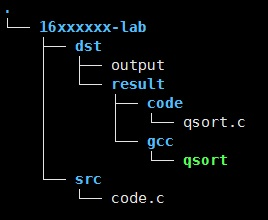
\includegraphics[height=4cm]{0-exam}
\end{figure}

\section{实验思考}
\begin{itemize}
\item \hyperref[think-Shell简析]{\textbf{\textcolor{baseB}{思考-Shell简析}}}
\item \hyperref[think-文件的操作]{\textbf{\textcolor{baseB}{思考-文件的操作}}}
\item \hyperref[think-箭头与指令]{\textbf{\textcolor{baseB}{思考-箭头与指令}}}
\item \hyperref[think-小明的困境]{\textbf{\textcolor{baseB}{思考-小明的困境}}}
\item \hyperref[think-克隆]{\textbf{\textcolor{baseB}{思考-克隆命令}}}
\end{itemize}

请认真做练习,然后把实验思考里的内容附在实验文档中一起提交!

\chapter{内核、Boot和printf}

\section{实验目的}
  \begin{enumerate}
    \item 掌握操作系统实验所需的基本工具
    \item 从操作系统角度理解MIPS体系结构
    \item 掌握操作系统启动的基本流程
  \end{enumerate}
在本章中,我们需要阅读并填写部分代码,使得我们的小操作系统可以正常的运行起来。这一章节的难度较为简单,
主要是为了让大家熟悉操作系统实验环境中的各类工具,为后续的实验奠定基础。
    
\section{操作系统的启动}

\subsection{内核在哪里?}
通过《计算机组成原理》课的学习,我们知道计算机是由硬件和软件组成的,仅有一个裸机是什么也干不了的;
另一方面,软件也必须运行在硬件之上才能实现其价值。由此可见,硬件和软件是相互依存、密不可分的。
为了能较好的管理计算机系统的硬件资源,我们需要使用操作系统。
而操作系统本身也是一种软件,我们可能会有这样的疑问:我们运行的Hello World程序是通过操作系统的机制实现的,
那么操作系统这种软件又是如何启动起来的呢?

\begin{note}
操作系统的启动英文称作“boot”。这个词是bootstrap的缩写,意思是鞋带(靴子上的那种)。
之所以将操作系统启动称为boot,源自于一个英文的成语“pull oneself up by one's bootstraps”,
直译过来就是用自己的鞋带把自己提起来。操作系统启动的过程正是这样一个极度纠结的过程。
硬件是在软件的控制下执行的,而当刚上电的时候,存储设备上的软件又需要由硬件载入到内存中去执行。
可是没有软件的控制,谁来指挥硬件去载入软件?因此,就产生了一个类似于鸡生蛋,蛋生鸡一样的问题。
硬件需要软件控制,软件又依赖硬件载入。就好像要用自己的鞋带把自己提起来一样。
早期的工程师们在这一问题上消耗了大量的精力。所以,他们后来将“启动”这一纠结的过程称为“boot”。
\end{note}

操作系统最重要的部分是操作系统内核,因为内核需要直接与硬件交互,从而利用硬件的功能为用户进程提供服务。
我们知道一个程序要能够运行,其代码必须能够被CPU直接访问,所以不能在磁盘上,因为CPU无法直接访问磁盘;
另一方面,内存RAM是易失性存储器,掉电后将丢失全部数据,所以不可能将内核代码保存在内存中。
所以直观上想,内核文件有可能放置的位置只能是CPU能够直接访问的非易失性存储器——ROM或FLASH中。

但是,把操作系统内核放置在这种非易失存储器上会有一些问题:
\begin{enumerate}
  \item 这种CPU能直接访问的非易失性存储器的存储空间一般会映射到CPU寻址空间的某个区域,这个是在硬件设计上决定的。
显然这个区域的大小是有限的,如果功能比较简单的操作系统还能够放在其中,对于内核文件较大的普通操作系统而言显然是不足够的。
  \item 如果操作系统内核在CPU加电后直接启动,意味着一个计算机硬件上只能启动一个操作系统,这样的限制显然不是我们所希望的。
  \item 把特定硬件相关的代码全部放在操作系统中也不利于操作系统的移植工作。
\end{enumerate}

基于上述考虑,设计人员一般都会将硬件初始化的相关工作放在名为“bootloader”的程序中来完成。这样做的好处正对应上述的问题:
\begin{enumerate}
  \item 将硬件初始化的相关工作从操作系统中抽出放在bootloader中实现,意味着通过这种方式实现了硬件启动和软件启动的分离。
因此需要存储在非易失性存储器中的硬件启动相关指令不需要很多,能够很容易地保存在ROM或FLASH中。
  \item bootloader在硬件初始化完后,需要为软件启动(即操作系统内核的功能)做相应的准备,
比如需要将内核镜像文件从存放它的存储器(比如磁盘)中读到RAM中。既然bootloader需要将内核镜像文件加载到内存中,
那么它就能选择使用哪一个内核镜像进行加载,即实现多重开机的功能。使用bootloader后,我们就能够在一个硬件上运行多个操作系统了。
  \item bootloader主要负责硬件启动相关工作,同时操作系统内核则能够专注于软件启动以及对用户提供服务的工作,
从而降低了硬件相关代码和软件相关代码的耦合度,有助于操作系统的移植。需要注意的是这样做并不意味着操作系统不依赖硬件。
由于操作系统直接管理着计算机所有的硬件资源,要想操作系统完全独立于处理器架构和硬件平台显然是不切实际的。
然而使用bootloader更清晰地划分了硬件启动和软件启动的边界,使操作系统与硬件交互的抽象层次提高了,从而简化了操作系统的开发和移植工作。
\end{enumerate}

\subsection{Bootloader}
从操作系统的角度看,boot loader 的总目标就是正确地调用内核来执行。
另外,由于 boot loader 的实现依赖于 cpu 的体系结构,因此大多数boot loader 都分为 stage1 和 stage2两大部分。

在stage 1时,此时需要初始化硬件设备,包括watchdog timer、中断、时钟、内存等。需要注意的一个细节是,此时内存RAM尚未初始化完成,
因而stage 1直接运行在存放bootloader的存储设备上(比如FLASH)。由于当前阶段不能在内存RAM中运行,其自身运行会受诸多限制,
比如有些flash程序不可写,即使程序可写的flash也有存储空间限制。这就是为什么需要stage 2的原因。
stage 1除了初始化基本的硬件设备以外,会为加载stage 2准备RAM空间,然后将stage 2的代码复制到RAM空间,并且设置堆栈,最后跳转到stage 2的入口函数。

stage 2运行在RAM中,此时有足够的运行环境从而可以用C语言来实现较为复杂的功能。
这一阶段的工作包括,初始化这一阶段需要使用的硬件设备以及其他功能,然后将内核镜像文件从存储器读到RAM中,并为内核设置启动参数,
最后将CPU指令寄存器的内容设置为内核入口函数的地址,即可将控制权从bootloader转交给操作系统内核。

从CPU上电到操作系统内核被加载的整个启动的步骤如图\ref{fig:bootloader-steps}所示。

\begin{figure}[htbp]
  \centering
  \includegraphics[width=10cm]{bootloader-steps}
  \caption{启动的基本步骤}\label{fig:bootloader-steps} 
\end{figure}

需要注意的是,以上bootloader的两个工作阶段只是从功能上论述内核加载的过程,在具体实现上不同的系统可能有所差别,而且对于不同的硬件环境也会有些不同。
在我们常见的x86 PC的启动过程中,首先执行的是BIOS中的代码,主要完成硬件初始化相关的工作,
然后BIOS会从MBR(master boot record,开机硬盘的第一个扇区)中读取开机信息。在Linux中常说的Grub和Lilo这两种开机管理程序就是保存在MBR中。

\begin{note}
GRUB(GRand Unified Bootloader)是GNU项目的一个多操作系统启动程序。简单的说,就是可以可以用于在有多个操作系统的机器上,
在刚开机的时候选择一个操作系统进行引导。如果安装过Ubuntu一类的发行版的话, 一开机出现的那个选择系统用的菜单就是GRUB提供的。
\end{note}

(这里以Grub为例)BIOS加载MBR中的Grub代码后就把CPU交给了Grub,Grub的工作就是一步一步的加载自身代码,从而识别文件系统,
然后就能够将文件系统中的内核镜像文件加载到内存中,并将CPU控制权转交给操作系统内核。
这样看来,其实BIOS和Grub的前一部分构成了前述stage 1的工作,而stage 2的工作则是完全在Grub中完成的。

\begin{note}
bootloader有两种操作模式:启动加载模式和下载模式。对于普通用户而言,bootloader只运行在启动加载模式,就是我们之前讲解的过程。
而下载模式仅仅对于开发人员有意义,区别是前者是通过本地设备中的内核镜像文件启动操作系统的,而后者是通过串口或以太网等通信手段将远端的内核镜像上载到内存的。
\end{note}

\subsection{gxemul中的启动流程}
从前面的分析,我们可以看到,操作系统的启动是一个非常复杂的过程。不过,幸运的是,由于我们的小操作系统的目标是在gxemul仿真器上运行,
这个过程被大大简化了。gxemul仿真器支持直接加载elf格式的内核,也就是说,gxemul已经提供了bootloader全部功能。
我们的小操作系统不需要再实现bootloader的功能了。换句话说,你可以假定,从我们的小操作系统的运行第一行代码前,
我们就已经拥有一个正常的C环境了。全局变量、函数调用等等C语言运行所需的功能已经可以正常使用了。

\begin{note}
如果你以前对于操作系统的概念仅仅停留在很表面的层次上,那么这里你也许会有所疑惑,为什么我们这里要说“正常的C环境”?
难道还能有“不正常的C环境”?我们来举一个例子说明一下:假定我们刚加电,CPU开始从ROM上取指。
为了简化,我们假定这台机器上没有BIOS(Basic Input Output System),bootloader被直接烧在了ROM中(很多嵌入式环境就是这样做的)。
这时,由于内存没有被初始化,整个bootloader程序尚处于ROM中。程序中的全局变量也仍被储存在ROM上。
而ROM是只读的,所以任何对于全局变量的赋值操作都是不被允许的。可见,此时我们尚不能正常使用C语言的一些特性。
而当内存被初始化,bootloader将后续代码载入到内存中后,位于内存中的代码便能完整地使用C语言的各类功能了。
所以说,内存中的代码拥有了一个正常的C环境。
\end{note}

gxemul支持加载elf格式内核,所以启动流程被简化为加载内核到内存,之后跳转到内核的入口。启动完毕:)整个启动过程非常简单。
这里要注意,之所以简单还有一个原因就在于gxemul本身是仿真器,是一种软件而不是真正的硬件,
所以就不需要面对传统的bootloader面对的那种非常纠结的情况了。

\section{Let's hack the kernel!}

接下来,我们就要开始来折腾我们的小操作系统内核了。这一节中,我们将介绍如何修改内核并实现一些自定义的功能。

\subsection{Makefile——内核代码的地图}
当我们想要翻开代码大干一番的时候,却面临着一个天大的问题:这堆代码应当从何读起?答曰:Makefile。当你不知所措的时候,
从Makefile开始往往会是一个不错的选择。这时,有同学要问了:什么是make?什么又是Makefile呢?
make工具一般用于维护工程。它可以根据时间戳自动判断项目的哪些部分是需要重新编译的,每次只重编译必要的部分。make工具会读取Makefile文件,
并根据Makefile的内容来执行相应的编译操作。Makefile类似于大家以前接触过的VC工程文件。只不过不像VC那样有图形界面,而是直接用类似脚本的方式实现的。

\begin{note}
相较于VC工程而言,Makefile具有更高的\textbf{灵活性}(当然,高灵活性的代价就是学习成本会有所提升,这是必然的),可以方便地管理大型的项目。
而且Makefile理论上支持\textbf{任意的语言},只要其编译器可以通过shell命令来调用。当你的项目可能会混合多种语言,有着复杂的构建流程的时候,
Makefile便能展现出它真正的威力来。
\end{note}

为了使你更为清晰地了解Makefile的基本概念,我们来写一个简单的Makefile。假设我们手头有一个Hello World程序需要编译。我们来为它写一个简易的Makefile。
让我们从头开始,如果我们没有Makefile,直接动手编译这个程序,我们需要下面这样一个指令

\begin{minted}[linenos]{bash}
# 直接使用gcc编译Hello World程序
$ gcc -o hello_world hello_world.c
\end{minted}

那么,如果我们想把它写成Makefile,我们应该怎么办呢?makefile最基本的格式是这样的

\begin{minted}[linenos]{make}
target: dependencies
    command 1
    command 2
    ...
    command n
\end{minted}

其中,target是我们构建(Build)的目标,而dependencies是构建该目标所需的其它文件或其他目标。之后是构建出该目标所需执行的指令。
有一点尤为需要注意:\textbf{每一个指令(command)之前必须有一个TAB}。这里必须使用TAB而不能是空格,否则make会报错。

我们的简易的Makefile可以写成如下的样子,之后执行make即可产生hello\_world这个可执行文件。

\begin{minted}[linenos]{make}
all: hello_world.c
    gcc -o hello_world hello_world.c
\end{minted}

理解了Makefile最基本的概念后,我们来看一下我们的小操作系统的最顶层的Makefile。由于Makefile是用于指导程序如何被构建的,
因此,通过阅读Makefile,我们就可以理解源代码被构建成可执行文件的过程。这一过程可以给我们一些阅读代码的提示,
可以说,Makefile就像源代码的地图,告诉你源代码是如何一步一步成为最终的可执行文件的。代码\ref{code:top-makefile}是实验代码最顶层的Makefile,
通过阅读它我们就能了解代码中很多宏观的东西。

\begin{codeBoxWithCaption}{顶层Makefile\label{code:top-makefile}}
  \inputminted[linenos]{make}{codes/top-Makefile}
\end{codeBoxWithCaption}

如果你以前没有接触过Makefile的话,突然看到这份40行的Makefile可能会有些无奈,完全看不懂啊。不必着急,我们来一行一行地解读它。
前6行是注释,你懂得。7~21行定义了一些变量,包括各个子目录的相对路径,最终的可执行文件的路径(vmlinux\_elf),
linker script的位置(link\_script)。值得注意的两个是modules定义了内核所包含的所有模块,而objects则表示要编译出内核所依赖的所有.o文件。
17到21行行末的斜杠代表这一行没有结束,下一行的内容和这一行是连在一起的。这种写法一般用于提高文件的可读性。可以把本该写在同一行的东西分布在多行中,
使得文件更容易被人类阅读。

\begin{note}
linker script是用于指导连接器将多个.o文件连接成目标可执行文件的脚本。.o文件、linker script等内容我们会在下面的小节中细致地讲解,
大家这里只要知道这些文件是编译内核所必要的就好。
\end{note}

23行的.PHONY表明列在其后的规则不受修改时间的约束。也就是说,一旦该规则被调用,一定保证它被执行。第25行定义all这一规则的依赖。
all代表整个项目,由此我们可以知道,构建整个项目依赖于构建好所有的模块以及vmlinux。那么vmlinux是如何被构建的呢?
紧接着的27行定义了,vmlinux的构建依赖于所有的模块。在构建完所有模块后,将执行第28行的指令来产生vmlinux。
我们可以看到,第28行调用了连接器将之前构建各模块产生的所有.o文件在linker script的指导下连接到一起,产生最终的vmlinux可执行文件。
第30行定义了每个模块的构建方法为调用对应模块目录下的Makefile。最后的33到38行定义了如何清理所有被构建出来的文件。

\begin{note}
一般在写Makefile时,习惯将第一个规则命名为all,也就是构建整个项目的意思。如果调用make时没有指定目标,make会自动执行第一个目标,
所以把all放在第一个目标的位置上,可以使得make命令默认构建整个项目,较为方便。
\end{note}

读到这里,我们会发现还有几个关键的变量没有定义。是的,就是LD、MAKE等出现在编译指令中的变量。紧接着我们看到了第40行有一条include命令。
看来,这个顶层的Makefile还引用了其他的东西。显然这些未定义的变量,是被定义在了这个被include的文件中。被引用的文件如代码\ref{code:include-mk}所示。

\begin{codeBoxWithCaption}{include.mk\label{code:include-mk}}
  \inputminted[linenos]{make}{codes/include.mk}
\end{codeBoxWithCaption}

在该文件中,我们看到了一个非常熟悉的关键词——Cross Compile(交叉编译)。不难看出,这里的CROSS\_COMPILE变量是在定义编译和连接等指令的前缀,
或者说是交叉编译器的具体位置。例如,LD最终调用的指令是“/opt/eldk/usr/bin/mips\_4KC-ld”。通过修改该变量,就可以方便地设定交叉编译工具链的位置。

\begin{exercise}
请修改include.mk文件,使交叉编译器的路径正确。之后执行make指令,如果配置一切正确,则会在gxemul目录下生成vmlinux的内核文件。
\end{exercise}

至此,我们就可以大致掌握阅读Makefile的方法了。善于运用make的功能可以给你带来很多惊喜哦:)提示:可以试着使用一下make clean。
如果你觉得每次用gxemul运行内核都需要打很长的指令这件事很麻烦,那么可以尝试在Makefile中添加运行内核这一功能,使得通过make就能自动运行内核。

\subsection{ELF——深入探究编译与链接}
如果你已经尝试过运行内核,那么你会发现它现在是根本运行不起来的。因为我们还有一些重要的步骤没有做。但是在做这些之前,我们不得不补充一些重要的,
但又有些琐碎的知识。在这里,我们将掀开可执行文件的神秘面纱,进一步去了解一段代码是如何从编译一步一步变成一个可执行文件以及可执行文件又是如何被执行的。

在一切开始之前,请你先泡好一杯茶,慢慢地、耐心地读下去。这一部分的知识对于后面十分重要,但又十分冗长。我们会尽量说得轻松活泼一些,
但由于知识本身的琐碎以及不连贯,所以阅读体验并不会很好。请务必坚持看完:)

\begin{codeBoxWithCaption}{一个简单的C程序\label{code:hello-c}}
  \inputminted[linenos]{c}{codes/hello.c}
\end{codeBoxWithCaption}

我们以代码\ref{code:hello-c}为例,讲述我们这个冗长的故事。我们首先探究这样一个问题:\textbf{含有多个C文件的工程是如何编译成一个可执行文件的?}

这段代码相信你非常熟悉了,不知你有没有注意到过这样一个小细节:printf的定义在哪里?
\footnote{printf位于标准库中,而不在我们的C代码中。将标准库和我们自己编写的C文件编译成一个可执行文件的过程,与将多个C文件编译成一个可执行文件的过程相仿。
因此,我们通过探究printf如何和我们的C文件编译到一起,来展示整个过程。}
我们都学过,C语言中函数必须有定义才能被调用,那么printf的定义在哪里呢?你一定会笑一笑说,别傻了,不就在stdio.h中吗?我们在程序开头通过include引用了它的。
然而事实真的是这样吗?我们来进去看一看stdio.h里到底有些什么。

\begin{codeBoxWithCaption}{stdio.h中关于printf的内容\label{code:part-stdio-h}}
  \inputminted[linenos]{c}{codes/part_of_stdio.h}
\end{codeBoxWithCaption}

在代码\ref{code:part-stdio-h}中,我们展示了从当前系统的stdio.h中摘录出的与printf相关的部分。可以看到,我们所引用的stdio.h中只有声明,但并没有printf的定义。
或者说,并没有printf的具体实现。可没有具体的实现,我们究竟是如何调用printf的呢?我们怎么能够调用一个没有实现的函数呢?

我们来一步一步探究,printf的实现究竟被放在了哪里,又究竟是在何时被插入到我们的程序中的。首先,我们要求编译器\textbf{只进行预处理(通过-E选项)},而不编译。

\begin{minted}[linenos]{c}
/* 由于原输出太长,这里只能留下很少很少的一部分。 */
typedef unsigned char __u_char;
typedef unsigned short int __u_short;
typedef unsigned int __u_int;
typedef unsigned long int __u_long;


typedef signed char __int8_t;
typedef unsigned char __uint8_t;
typedef signed short int __int16_t;
typedef unsigned short int __uint16_t;
typedef signed int __int32_t;
typedef unsigned int __uint32_t;

typedef signed long int __int64_t;
typedef unsigned long int __uint64_t;

extern struct _IO_FILE *stdin;
extern struct _IO_FILE *stdout;
extern struct _IO_FILE *stderr;

extern int printf (const char *__restrict __format, ...);

int main()
{
    printf("Hello World!\n");
    return 0;
}
\end{minted}

可以看到,C语言的预处理器将头文件的内容添加到了源文件中,但同时我们也能看到,这里一阶段并没有printf这一函数的定义。

之后,我们将gcc的-E选项换为-c选项,\textbf{只编译而不链接},产生一个.o目标文件。
我们对其进行反汇编\footnote{为了便于你重现,我们这里没有选择MIPS,而选择了在流行的x86-64体系结构上进行反汇编。
同时,由于x86-64的汇编是CISC汇编,看起来会更为清晰一些。},结果如下

\begin{minted}[linenos]{objdump}
hello.o:     file format elf64-x86-64

Disassembly of section .text:

0000000000000000 <main>:
   0:   55                      push   %rbp
   1:   48 89 e5                mov    %rsp,%rbp
   4:   bf 00 00 00 00          mov    $0x0,%edi
   9:   e8 00 00 00 00          callq  e <main+0xe>
   e:   b8 00 00 00 00          mov    $0x0,%eax
  13:   5d                      pop    %rbp
  14:   c3                      retq
\end{minted}

我们只需要注意中间那句callq即可,这一句是调用函数的指令。对照左侧的机器码,其中e8是call指令的操作码。根据我们在《计算机组成》课程中学习MIPS跳转指令的经验,
e8后面应该跟的是printf的地址。可在这里我们却发现,\textbf{本该填写printf地址的位置上被填写了一串0}。那个地址显然不可能是printf的地址。也就是说,直到这一步,
printf的具体实现依然不在我们的程序中。

最后,我们允许gcc进行连接,也就是\textbf{正常地编译}出可执行文件。然后,再用objdump进行反汇编。

\begin{minted}[linenos]{objdump}
hello:     file format elf64-x86-64


Disassembly of section .init:

00000000004003a8 <_init>:
  4003a8:       48 83 ec 08             sub    $0x8,%rsp
  4003ac:       48 8b 05 0d 05 20 00    mov    0x20050d(%rip),%rax
  4003b3:       48 85 c0                test   %rax,%rax
  4003b6:       74 05                   je     4003bd <_init+0x15>
  4003b8:       e8 43 00 00 00          callq  400400 <__gmon_start__@plt>
  4003bd:       48 83 c4 08             add    $0x8,%rsp
  4003c1:       c3                      retq   

Disassembly of section .plt:

00000000004003d0 <puts@plt-0x10>:
  4003d0:       ff 35 fa 04 20 00       pushq  0x2004fa(%rip)
  4003d6:       ff 25 fc 04 20 00       jmpq   *0x2004fc(%rip)
  4003dc:       0f 1f 40 00             nopl   0x0(%rax)

00000000004003e0 <puts@plt>:
  4003e0:       ff 25 fa 04 20 00       jmpq   *0x2004fa(%rip)
  4003e6:       68 00 00 00 00          pushq  $0x0
  4003eb:       e9 e0 ff ff ff          jmpq   4003d0 <_init+0x28>

00000000004003f0 <__libc_start_main@plt>:
  4003f0:       ff 25 f2 04 20 00       jmpq   *0x2004f2(%rip)
  4003f6:       68 01 00 00 00          pushq  $0x1
  4003fb:       e9 d0 ff ff ff          jmpq   4003d0 <_init+0x28>

0000000000400400 <__gmon_start__@plt>:
  400400:       ff 25 ea 04 20 00       jmpq   *0x2004ea(%rip)
  400406:       68 02 00 00 00          pushq  $0x2
  40040b:       e9 c0 ff ff ff          jmpq   4003d0 <_init+0x28>

Disassembly of section .text:

0000000000400410 <main>:
  400410:       48 83 ec 08             sub    $0x8,%rsp
  400414:       bf a4 05 40 00          mov    $0x4005a4,%edi
  400419:       e8 c2 ff ff ff          callq  4003e0 <puts@plt>
  40041e:       31 c0                   xor    %eax,%eax
  400420:       48 83 c4 08             add    $0x8,%rsp
  400424:       c3                      retq   

0000000000400425 <_start>:
  400425:       31 ed                   xor    %ebp,%ebp
  400427:       49 89 d1                mov    %rdx,%r9
  40042a:       5e                      pop    %rsi
  40042b:       48 89 e2                mov    %rsp,%rdx
  40042e:       48 83 e4 f0             and    $0xfffffffffffffff0,%rsp
  400432:       50                      push   %rax
  400433:       54                      push   %rsp
  400434:       49 c7 c0 90 05 40 00    mov    $0x400590,%r8
  40043b:       48 c7 c1 20 05 40 00    mov    $0x400520,%rcx
  400442:       48 c7 c7 10 04 40 00    mov    $0x400410,%rdi
  400449:       e8 a2 ff ff ff          callq  4003f0 <__libc_start_main@plt>
  40044e:       f4                      hlt    
  40044f:       90                      nop
\end{minted}

篇幅所限,余下的部分没法再展示了(大约还有100来行)。当你看到这段代码的时候,心头一定有一大群草泥马呼啸而过。
什么鬼!我们原本那只可爱的Hello World怎么变成了这副鬼样子!

别急,我们还是只把注意力放在主函数中,这一次,我们可以看到,主函数里那一句callq后面已经不再是一串0了。
那里已经\textbf{被填入了一个地址}。从反汇编代码中我们也可以看到,这个地址就在这个可执行文件里,就在被标记为puts@plt的那个位置上。
虽然高不清楚那货是什么,但显然那就是我们所调用的printf的具体实现了。

由此,我们不难推断,printf的实现是在\textbf{连接(Link)}这一步骤中被插入到最终的可执行文件中的。那么,了解这个细节究竟有什么用呢?
作为一个库函数,printf被大量的程序所使用。因此,每次都将其编译一遍实在太浪费时间了。printf的实现其实早就被编译成了二进制形式。
但此时,printf并未连接到程序中,它的状态与我们利用-c选项产生的hello.o相仿,都还处于未连接的状态。而在编译的最后,
连接器(Linker)会将所有的目标文件连接在一起,将之前未填写的地址等信息填上,形成最终的可执行文件,这就是连接的过程。

对于拥有多个c文件的工程来说,编译器会首先将所有的c文件以文件为单位,编译成.o文件。最后再将所有的.o文件以及函数库连接在一起,
形成最终的可执行文件。整个过程如图\ref{fig:link}所示。

\begin{figure}[htbp]
  \centering
  \includegraphics[width=8cm]{link}
  \caption{编译、连接的过程}\label{fig:link} 
\end{figure}

接下来,我们提出我们的下一个问题:\textbf{连接器通过哪些信息来连接多个目标文件呢?}答案就在于在目标文件(也就是我们通过-c选项生成的.o文件)。
在目标文件中,记录了代码各个段的具体信息。连接器通过这些信息来将目标文件链接到一起。而ELF(Executable and Linkable Format)正是Unix上常用的一种目标文件格式。
其实,不仅仅是目标文件,可执行文件也是使用ELF格式记录的。这一点通过ELF的全称也可以看出来。

为了帮助你了解ELF文件,下一步我们需要进一步探究它的功能以及格式。

ELF文件是一种对可执行文件、目标文件和库使用的文件格式,跟Windows下的PE文件格式类似。ELF格式是是UNIX系统实验室作为ABI(Application Binary Interface)而开发和发布的,现在早已经是Linux下的标准格式了。我们在之前曾经看见过的.o文件就是ELF所包含的三种文件类型中的一种,称为可重定位(relocatable)文件,其它两种文件类型分别是可执行(executable)文件和共享对象(shared object)文件,这两种文件都需要链接器对可重定位文件进行处理才能生成。

你可以使用file命令来获得文件的类型,如图\ref{fig:lab1-file}所示。

\begin{figure}[htbp]
  \centering
  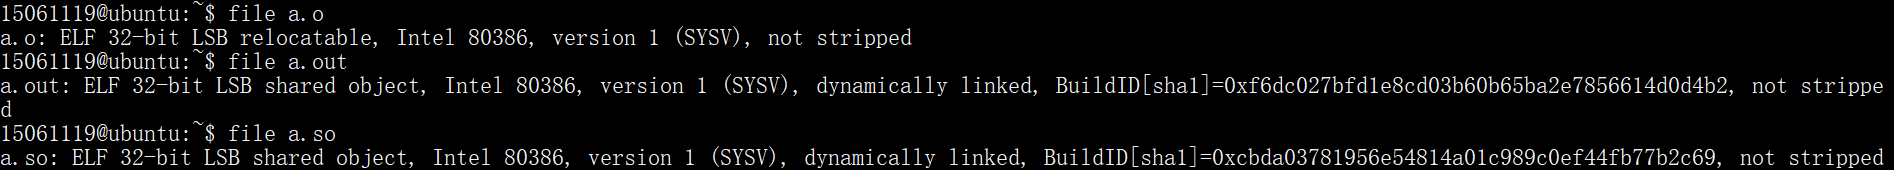
\includegraphics[width=18cm,height=6cm]{lab1-file}
  \caption{file命令}\label{fig:lab1-file} 
\end{figure}

那么,ELF文件中都包含有什么东西呢?简而言之,就是和程序相关的所有必要信息,下图\ref{fig:lab1-elf-1}说明了ELF文件的结构:

\begin{figure}[htbp]
  \centering
  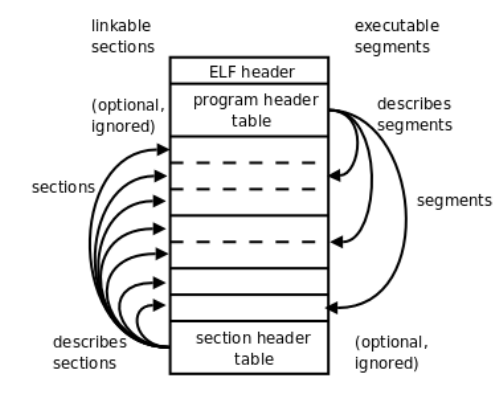
\includegraphics[width=8cm]{lab1-elf-1}
  \caption{ELF文件结构}\label{fig:lab1-elf-1}
\end{figure}

通过上图我们可以知道,ELF文件从整体来说包含5个部分:

\begin{enumerate}
  \item ELF Header,包括程序的基本信息,比如体系结构和操作系统,同时也包含了Section Header Table和Program Header Table相对文件的偏移量(offset)。
  \item Program Header Table,也可以称为Segment Table,主要包含程序中各个Segment的信息,Segment的信息需要在运行时刻使用。
  \item Section Header Table,主要包含各个Section的信息,Section的信息需要在程序编译和链接的时候使用。
  \item Segments,就是各个Segment。
  \item Sections,就是各个Section。
\end{enumerate}

观察上图\ref{fig:lab1-elf-1}我们可以发现,Program Header Table和Section Header Table指向了同样的地方,这就说明两者所代表的内容是重合的,这意味着什么呢?意味着两者只是同一个东西的不同视图!产生这种情况的原因在于ELF文件需要在两种场合使用:

  \begin{enumerate}
    \item 组成可重定位文件,参与可执行文件和可共享文件的链接。
    \item 组成可执行文件或者可共享文件,在运行时为加载器提供信息。
  \end{enumerate}

我们已经了解了ELF文件的大体结构,现在,我们需要你自己动手,阅读一个简易的ELF文件的解析程序,然后完成部分代码,来了解ELF文件各个部分的详细结构。

\begin{exercise}
阅读kerelf.h、readelf.c以及main.c三个文件中的代码,并完成readelf.c中缺少的代码,使得main.c程序可以正确编译和输出。
\end{exercise}

\begin{thinking}\label{think-endian}
也许你会发现我们的readelf程序是不能解析之前生成的内核文件(内核文件是可执行文件)的,这是为什么呢?我们把这个问题留给你来思考。
\end{thinking}

通过刚才的练习,相信你已经对ELF文件有了一个比较充分的了解,你可能想进一步解析ELF文件来获得更多的信息,不过这个工作已经有人帮你做了,使用readelf工具,你就可以很方便地解析ELF文件。
现在,我们继续内核的话题。

我们最终生成的内核也是ELF格式的,被模拟器载入到内核中。因此,我们暂且只关注ELF是如何被载入到内核中,并且被执行的,
而不再关心具体的连接细节。ELF中有两个相似却不同的概念segment和section,我们之前已经提到过,section记录了程序的代码段、数据段等各个段的内容,
主要是连接器在连接的过程中需要使用。而segment则记录了每一段数据(包括代码等内容)需要被载入到哪里,记录了用于指导应用程序加载的各类信息。

我们不妨来看一下,我们之前那个hello world程序的各个segment长什么样子。readelf工具可以方便地解析出elf文件的内容,这里我们使用它来分析我们的程序。

\begin{minted}[linenos]{objdump}
Elf 文件类型为 EXEC (可执行文件)
入口点 0x400e6e
共有 5 个程序头,开始于偏移量64

程序头:
  Type           Offset             VirtAddr           PhysAddr
                 FileSiz            MemSiz              Flags  Align
  LOAD           0x0000000000000000 0x0000000000400000 0x0000000000400000
                 0x00000000000b33c0 0x00000000000b33c0  R E    200000
  LOAD           0x00000000000b4000 0x00000000006b4000 0x00000000006b4000
                 0x0000000000001cd0 0x0000000000003f48  RW     200000
  NOTE           0x0000000000000158 0x0000000000400158 0x0000000000400158
                 0x0000000000000044 0x0000000000000044  R      4
  TLS            0x00000000000b4000 0x00000000006b4000 0x00000000006b4000
                 0x0000000000000020 0x0000000000000050  R      8
  GNU_STACK      0x0000000000000000 0x0000000000000000 0x0000000000000000
                 0x0000000000000000 0x0000000000000000  RW     10

 Section to Segment mapping:
  段节...
   00     .note.ABI-tag .note.gnu.build-id .rela.plt .init .plt .text 
   __libc_freeres_fn __libc_thread_freeres_fn .fini .rodata __libc_subfreeres 
   __libc_atexit __libc_thread_subfreeres .eh_frame .gcc_except_table 
   01     .tdata .init_array .fini_array .jcr .data.rel.ro .got .got.plt .data 
   .bss __libc_freeres_ptrs 
   02     .note.ABI-tag .note.gnu.build-id 
   03     .tdata .tbss 
   04
\end{minted}

这些输出中,我们只需要关注这样几个部分:Offset代表该段(segment)的数据相对于ELF文件的偏移。VirtAddr代表该段最终需要被加载到内存的哪个位置。
FileSiz代表该段的数据在文件中的长度。MemSiz代表该段的数据在内存中所应当占的大小。

\begin{note}
MemSiz永远大于等于FileSiz。若MemSiz大于FileSiz,则操作系统在加载程序的时候,会首先将文件中记录的数据加载到对应的VirtAddr处。
之后,向内存中填0,直到该段在内存中的大小达到MemSiz为止。那么为什么MemSiz有时候会大于FileSiz呢?这里举这样一个例子:
C语言中未初始化的全局变量,我们需要为其分配内存,但它又不需要被初始化成特定数据。因此,在可执行文件中也只记录它需要占用内存(MemSiz),
但在文件中却没有相应的数据(因为它并不需要初始化成特定数据)。故而在这种情况下,MemSiz会大于FileSiz。这也解释了,
为什么C语言中全局变量会有默认值0。这是因为操作系统在加载时将所有未初始化的全局变量所占的内存统一填了0。
\end{note}

VirtAddr是我们尤为需要注意的。由于它的存在,我们就不难推测,Gxemul仿真器在加载我们的内核时,是按照内核这一可执行文件中所记录的地址,
将我们内核中的代码、数据等加载到相应位置。并将CPU的控制权交给内核。我们的内核之所以不能够正常运行,显然是因为我们内核所处的地址是不正确的。
换句话说,\textbf{只要我们能够将内核加载到正确的位置上,我们的内核就应该可以运行起来。}

思考到这里,我们又发现了两个重要的问题。
\begin{enumerate}
  \item 什么叫做正确的位置?到底放在哪里才叫正确。
  \item 哪个段被加载到哪里是记录在编译器编译出来的ELF文件里的,我们怎么才能修改它呢?
\end{enumerate}
在接下来的小节中,我们将一点一点解决掉这两个问题。

\subsection{MIPS内存布局——寻找内核的正确位置}
在这一节中,我们来解决关于内核应该被放在何处的问题。在32位的MIPS CPU中,程序地址空间会被划分为4个大区域。如图\ref{fig:memory-region}所示。

\begin{figure}[htbp]
  \centering
  \includegraphics[height=8cm]{memory-region}
  \caption{MIPS内存布局}\label{fig:memory-region} 
\end{figure}

从硬件角度讲,这四个区域的情况如下:

\begin{enumerate}
  \item User Space(kuseg) 0x00000000-0x7FFFFFFF(2G):这些是用户模式下可用的地址。在使用这些地址的时候,程序会通过MMU映射到实际的物理地址上。
  \item Kernel Space Unmapped Cached(kseg0) 0x80000000-0x9FFFFFFF(512MB):只需要将地址的高3 位清零,这些地址就被转换为物理地址。
也就是说,逻辑地址到物理地址的映射关系是硬件直接确定,不通过MMU。因为转换很简单,我们常常把这些地址称为“无需转换的”。
一般情况下,都是通过cache 对这段区域的地址进行访问。
  \item Kernel Space Unmapped Uncached(kseg1) 0xA0000000-0xBFFFFFFF(512MB):这一段地址的转换规则与前者相似,
通过将高3 位清零的方法将地址映射为相应的物理地址,然后映射到物理内存中512MB 大小的低字段。需要注意的是,kseg1 不通过cache 进行存取。
  \item Kernel Space Mapped Cached(kseg2) 0xC0000000-0xFFFFFFFF(1GB):这段地址只能在内核态下使用并且需要MMU 的转换。
\end{enumerate}

看到这里,你也许又蔫儿了,还是完全不知道该把内核放在哪里呀!这里,我们再提供一个提示:需要通过MMU映射访问的地址得在建立虚拟内存机制后才能正常使用,
是由操作系统所管理的。因此,在载入内核时,我们只能选用不需要通过MMU的内存空间,因为此时尚未建立虚存机制。好了,满足这一条件的只有kseg0和kseg1了。
而kseg1是不经过cache的,一般用于访问外部设备。所以,我们的内核只能放在seg0了。

那么具体放在哪里呢?这时,我们就需要仔细阅读代码了。在include/mmu.h里有我们的小操作系统内核完整的内存布局图(代码\ref{code:memory-mmu-h}所示),
在之后的实验中,善用它可以带来意料之外的惊喜。

\begin{codeBoxWithCaption}{include/mmu.h中的内存布局图\label{code:memory-mmu-h}}
  \inputminted[linenos]{c}{codes/memory-mmu.h}
\end{codeBoxWithCaption}

相信聪明的你已经发现了内核的正确位置了吧?

\subsection{Linker Script——控制加载地址}
在发现了内核的正确位置后,我们只需要想办法让内核被加载到那里就OK了。之前在分析ELF文件时我们曾看到过,编译器在生成ELF文件时就已经记录了各段所需要被加载到的位置。
同时,我们也发现,最终的可执行文件实际上是由连接器产生的(它将多个目标文件连接产生最终可执行文件)。因此,我们所需要做的,就是控制连接器的连接过程。

接下来,我们就要引入一个神奇的东西:Linker Script。连接器的设计者们在设计连接器的时候面临这样一个问题:不同平台的ABI(Application Binary Interface)都不一样,
怎样做才能增加连接器的通用性,使得它能为各个不同的平台生成可执行文件呢?于是,就有了Linker Script。Linker Script中记录了各个section应该如何映射到segment,
以及各个segment应该被加载到的位置。下面的指令可以输出默认的连接脚本,你可以在自己的机器上尝试这一条指令:

\begin{minted}[linenos]{bash}
ld --verbose
\end{minted}

这里,我们再补充一下关于ELF文件中section的概念。在链接过程中,目标文件被看成section的集合,并使用section header table来描述各个section的组织。
换句话说,section记录了在连接过程中所需要的必要信息。其中最为重要的三个段为.text、.data、.bss。这三种段的意义是必须要掌握的:

\begin{description}
  \item[.text] 保存可执行文件的操作指令。
  \item[.data] 保存已初始化的全局变量和静态变量。
  \item[.bss] 保存未初始化的全局变量和静态变量。
\end{description}

以上的描述也许会显得比较抽象,这里我们来做一个实验。我们编写一个用于输出代码、全局已初始化变量和全局未初始化变量地址的代码(如代码\ref{code:sections}所示)。
观察其运行结果与ELF文件中记录的.text、.data和.bss段相关信息之间的关系。

\begin{codeBoxWithCaption}{用于输出各section地址的程序\label{code:sections}}
  \inputminted[linenos]{c}{codes/sections.c}
\end{codeBoxWithCaption}

该程序的一个可能的输出如下\footnote{在不同机器上运行,结果也许会有一定的差异}。

\begin{minted}[linenos]{bash}
user@debian ~/Desktop $ ./program 
80D4188
80D60A0
8048AAC
\end{minted}

我们再看看ELF文件中记录的各section的相关信息(为了突出重点,这里只保留我们所关心的section)。

\begin{minted}[linenos]{objdump}
共有 29 个节头,从偏移量 0x9c258 开始:

节头:
  [Nr] Name              Type            Addr     Off    Size   ES Flg Lk Inf Al
  [ 4] .text             PROGBITS        08048140 000140 0620e4 00  AX  0   0 16
  [22] .data             PROGBITS        080d4180 08b180 000f20 00  WA  0   0 32
  [23] .bss              NOBITS          080d50c0 08c0a0 00136c 00  WA  0   0 64
\end{minted}

对比二者,我们就可以清晰的知道,\textbf{.text段包含了可执行文件中的代码},\textbf{.data段包含了需要被初始化的全局变量和静态变量},
而\textbf{.bss段包含了无需初始化的全局变量和静态变量}

接下来,我们通过Linker Script来尝试调整各段的位置。这里,我们选用GNU LD官方帮助文档上的例子
(\url{https://www.sourceware.org/binutils/docs/ld/Simple-Example.html#Simple-Example})
该例子的完整代码如下所示:

\begin{minted}[linenos]{objdump}
SECTIONS
{
   . = 0x10000;
   .text : { *(.text) }
   . = 0x8000000;
   .data : { *(.data) }
   .bss : { *(.bss) }
}
\end{minted}

在第三行的“.”是一个特殊符号,用来做定位计数器,它根据输出段的大小增长。在SECTIONS命令开始的时候,它的值为0。通过设置“.”即可设置接下来的section的其实地址。
“*”是一个通配符,匹配所有的相应的段。例如“.bss:\{*(.bss)\}”表示将所有输入文件中的.bss段(右边的.bss)都放到输出的.bss段(左边的.bss)中。
为了能够编译通过(这个脚本过于简单,难以用于连接真正的程序),我们将原来的实验代码简化如下

\begin{minted}[linenos]{c}
char msg[]="Hello World!\n";
int count;

int main()
{
    return 0;
}
\end{minted}

编译,并查看生产的可执行文件各section的信息。

\begin{minted}[linenos]{objdump}
user@debian ~/Desktop $ gcc -o test test.c -T test.lds -nostdlib -m32
user@debian ~/Desktop $ readelf -S test                              
共有 11 个节头,从偏移量 0x2164 开始:

节头:
  [Nr] Name              Type            Addr     Off    Size   ES Flg Lk Inf Al
  [ 2] .text             PROGBITS        00010024 001024 00000a 00  AX  0   0  1
  [ 5] .data             PROGBITS        08000000 002000 00000e 00  WA  0   0  1
  [ 6] .bss              NOBITS          08000010 00200e 000004 00  WA  0   0  4
\end{minted}

可以看到,在使用了我们自定义的Linker Script以后,生成的程序各个section的位置就被调整到了我们所指定的地址上。
segment是由section组合而成的,section的地址被调整了,那么最终segment的地址也会相应地被调整。
至此,我们就了解了如何通过lds文件控制各段被加载到的位置。

\begin{exercise}
填写tools/scse0\_3.lds中空缺的部分,将内核调整到正确的位置上。
\end{exercise}

再补充一点:关于链接后的程序从何处开始执行。程序执行的第一条指令称为entry point,
我们在linker script中可以通过ENTRY(function name)指令来设置程序入口。linker中程序入口的设置方法有以下五种:
\begin{enumerate}
  \item 使用ld命令时,通过参数“-e”设置
  \item 在linker scirpt中使用ENTRY()指令指定了程序入口
  \item 如果定义start,则start就是程序入口
  \item .text段的第一个字节
  \item 地址0处
\end{enumerate}
在我们的实验中,采用了其中的第二种方式指定了程序入口。

\section{MIPS汇编与C语言}
在这一节中,我们将简单介绍MIPS汇编,以及常见的C语言语法与汇编的对应关系。在操作系统编程中,不可避免地要接触到汇编语言。
我们经常需要从C语言中调用一些汇编语言写成的函数,或者反过来,在汇编中跳转到C函数。为了能够实现这些,
我们需要了解C语言与汇编之间千丝万缕的联系。

我们代码\ref{code:c-example}为例,介绍典型的C语言中的语句对应的汇编代码。

\begin{codeBoxWithCaption}{样例程序\label{code:c-example}}
  \inputminted[linenos]{c}{codes/example.c}
\end{codeBoxWithCaption}

\subsection{循环与判断}
这里你可能会问了,样例代码里只有循环啊!哪里有什么判断语句呀?事实上,由于MIPS汇编中没有循环这样的高级结构,
所有的循环均是采用判断加跳转语句实现的,所以我们将循环语句和判断语句合并在一起进行分析。
我们分析代码的第一步,就是要将循环等高级结构,用\textbf{判断加跳转}的方式替代。
例如,代码\ref{code:c-example}第13-15行的循环语句,其最终的实现可能就如下面的C代码所展示的那样。

\begin{minted}[linenos]{c}
      i = 0;
      goto CHECK;
FOR:  sum += fib(i);
      ++i;
CHECK:if (i < 10) goto FOR;
\end{minted}

将样例程序编译\footnote{为了生成更简单的汇编代码,我们采用了-nostdlib -static -mno-abicalls这三个编译参数},
我们观察其反汇编代码。对照汇编代码和我们刚才所分析出来的C代码。
我们基本就能够看出来其间的对应关系。这里,我们将对应的C代码标记在反汇编代码右侧。

\begin{minted}[linenos]{objdump}
  400158:       sw      zero,16(s8)           #       sum = 0;
  40015c:       sw      zero,20(s8)           #       i = 0;
  400160:       j       400190 <main+0x48>    #       goto CHECK;
  400164:       nop                           # --------------------
  400168:       lw      a0,20(s8)             #  FOR:
  40016c:       jal     4000b0 <fib>          #
  400170:       nop                           #
  400174:       move    v1,v0                 #        sum += fib(i);
  400178:       lw      v0,16(s8)             #
  40017c:       addu    v0,v0,v1              #
  400180:       sw      v0,16(s8)             #
  400184:       lw      v0,20(s8)             # --------------------
  400188:       addiu   v0,v0,1               #        ++i;
  40018c:       sw      v0,20(s8)             # --------------------
  400190:       lw      v0,20(s8)             # CHECK:
  400194:       slti    v0,v0,10              #        if (i < 10)
  400198:       bnez    v0,400168 <main+0x20> #            goto FOR;
  40019c:       nop
\end{minted}

再将右边的C代码对应会原来的C代码,我们就能够大致知道每一条汇编语句所对应的原始的C代码是什么了。
可以看出,判断和循环主要采用slt、slti判断两数间的大小关系,再结合b类型指令根据对应条件跳转。
以这些指令为突破口,我们就能大致识别出循环结构、分支结构了。

\subsection{函数调用}
这里需要区分函数的调用方和被调用方来分别分析。我们选用样例程序中的fib这个函数来观察函数调用相关的内容。
这个函数是一个递归函数,因此,它函数调用过程的调用者,同时也是被调用者。我们可以从中观察到如何调用一个函数,
以及一个被调用的函数应当做些什么工作。

我们还是先将整个函数调用过程用高级语言来表示一下。
\begin{minted}[linenos]{c}
int fib(int n)
{
        if (n == 0) goto BRANCH;
        if (n != 1) goto BRANCH2;
BRANCH: v0 = 1;
        goto RETURN;
BRANCH2:v0 = fib(n-1) + fib(n-2);
RETURN: return v0;
}
\end{minted}

然而,之后在分析汇编代码的时候,我们会发现有很多C语言中没有表示出来的东西。例如,在函数开头,有一大串的sw,
结尾处又有一大串的lw。这些东西究竟是在做些什么呢?

\begin{minted}[linenos]{objdump}
004000b0 <fib>:
  4000b0:       27bdffd8        addiu   sp,sp,-40
  4000b4:       afbf0020        sw      ra,32(sp)
  4000b8:       afbe001c        sw      s8,28(sp)
  4000bc:       afb00018        sw      s0,24(sp)
  # 中间暂且掠过,只关注一系列sw和lw操作。
  400130:       8fbf0020        lw      ra,32(sp)
  400134:       8fbe001c        lw      s8,28(sp)
  400138:       8fb00018        lw      s0,24(sp)
  40013c:       27bd0028        addiu   sp,sp,40
  400140:       03e00008        jr      ra
  400144:       00000000        nop
\end{minted}

我们来回忆一下C语言的递归。在经过了《数据结构》这门课程的学习后,你一定发现了,递归的过程和栈这种数据结构有着惊人的相似性。
每一次递归操作就仿佛将当前函数的所有变量和状态压入了一个栈中,待到返回时再从栈中弹出来。

好了,回忆起了这个细节,我们再来看看汇编代码。在函数的开头,编译器为我们添加了一组sw操作,
将所有当前函数所需要用到的寄存器原有的值全部保存到了内存中
\footnote{其实这样说并不准确,后面我们会看到,有些寄存器的值是由调用者负责保存的,有些是由被调用者保存的。但这里为了理解方便,
我们姑且认为被调用的函数保存了调用者的所有状态吧}。而在函数返回之前,编译器又加入了一组lw操作,将值被改变的寄存器全部恢复为原有的值。

我们惊奇地发现:编译器在函数调用的前后为我们添加了一组压栈(push)和弹栈(pop)的操作,为我们保存了函数的当前状态。
函数的开始,编译器首先\textbf{减小sp指针的值,为栈分配空间}。并将需要保存的值放置在栈中。
当函数将要返回时,编译器再\textbf{增加sp指针的值,释放栈空间}。同时,恢复之前被保存的寄存器原有的值。
这就是为何C语言的函数调用和栈有着很大的相似性的原因:在函数调用过程中,编译器真的为我们维护了一个栈。

\begin{note}
ra寄存器存放了函数的返回地址。使得被调用的函数结束时得以返回到调用者调用它的地方。但你有没有想过,我们其实可以将这个返回点设置为别的函数的入口,
使得该函数在返回时直接进入另一个函数中,而不是回到调用者哪里?一个函数调用了另一个函数,而返回时,返回到第三个函数中,
是不是也是一种很有价值的编程模型呢?如果你对此感兴趣,可以了解一下函数式编程中的Continuations的概念
(推荐\href{https://github.com/justinyhuang/Functional-Programming-For-The-Rest-of-Us-Cn/blob/master/FunctionalProgrammingForTheRestOfUs.cn.md}
{Functional Programming For The Rest Of Us}这篇文章),
在很多新近流行起来的语言中,都引入了类似的想法。
\end{note}

在我们看到了一个函数作为被调用者做了哪些工作后,我们再来看看,作为函数的调用者需要做些什么?如何调用一个函数?如何传递参数?又如何获取返回值?
让我们来看一下,fib函数调用fib(n-1)和fib(n-2)时,编译器为我们生成的汇编代码\footnote{为了方便你了解自己手写汇编时应当怎样写,我们这一次采用汇编代码,
而不是反汇编代码。这里注意,fp和上面反汇编出的s8其实是同一个寄存器,只是有两个不同的名字而已}

\begin{minted}[linenos]{gas}
lw      $2,40($fp)      # v0 = n;
addiu   $2,$2,-1        # v0 = a0 - 1;
move    $4,$2           # a0 = v0;      // 即a0=n-1
jal     fib             # v0 = fib(a0);
nop                     #

move    $16,$2          # s0 = v0;
lw      $2,40($fp)      # v0 = n;
addiu   $2,$2,-2        # v0 = n - 2;
move    $4,$2           # a0 = v0;      // 即a0=n-2
jal     fib             # v0 = fib(a0);
nop                     #

addu    $16,$16,$2      # s0 += v0;
sw      $16,16($fp)     #
\end{minted}

我们将汇编所对应的语义用C语言标明在右侧。可以看到,调用一个函数就是将参数存放在a0-a3寄存器中(我们暂且不关心参数非常多的函数会处理),
然后使用jal指令跳转到相应的函数中。函数的返回值会被保存在v0-v1寄存器中。我们通过这两个寄存器的值来获取返回值。

\begin{exercise}
完成boot/start.S中空缺的部分。设置栈指针,跳转到main函数。
使用gxemul –E testmips –C R3000 –M 64 elf-file运行(其中elf-file是你编译生成的vmlinux文件的路径)。 
\end{exercise}

在调用main函数之前,我们需要将sp寄存器设置到内核栈空间的位置上。具体的地址可以从mmu.h中看到。
这里做一个提醒,请注意栈的增长方向。设置完栈指针后,我们就具备了执行C语言代码的条件,因此,
接下来的工作就可以交给C代码来完成了。所以,在start.S的最后,我们调用C代码的主函数,
正式进入内核的C语言部分。

\subsection{通用寄存器使用约定}
为了和编译器等程序相互配合,我们需要遵循一些使用约定。这些规定与硬件无关,硬件并不关心寄存器具体被用于什么用途。
这些规定是为了让不同的软件之间得以协同工作而制定的。MIPS中一共有32个通用寄存器(General Purpose Registers),
其用途如表\ref{tab:registers}所示。

\begin{table}[h]
  \centering
  \begin{tabular}{ccp{10cm}}
    \toprule
    寄存器编号 & 助记符 & 用途 \\
    \midrule
    0   & zero & 值总是为0\\
    1   & at   & (汇编暂存寄存器)一般由汇编器作为临时寄存器使用。\\
    2-3 & v0-v1& 用于存放表达式的值或函数的整形、指针类型返回值\\
    4-7 & a0-a3& 用于函数传参。其值在函数调用的过程中不会被保存。若函数参数较多,多出来的参数会采用栈进行传递\\
    8-15& t0-t7& 用于存放表达式的值的临时寄存器;其值在函数调用的过程中不会被保存。\\
    16-23&s0-s7& 保存寄存器;这些寄存器中的值在经过函数调用后不会被改变。\\
    24-25&t8-t9& 用于存放表达式的值的临时寄存器;其值在函数调用的过程中不会被保存。当调用位置无关函数(position independent function)时,
               25号寄存器必须存放被调用函数的地址。\\
    26-27&kt0-kt1& 仅被操作系统使用。\\
    28  & gp   & 全局指针和内容指针。\\
    29  & sp   & 栈指针。\\
    30  &fp或s8& 保存寄存器(同s0-s7)。也可用作帧指针。\\
    31  & ra   & 函数返回地址。\\
    \bottomrule
  \end{tabular}
  \caption{MIPS通用寄存器\label{tab:registers}}
\end{table}

其中,只有16-23号寄存器和28-30号寄存器的值在函数调用的前后是不变的\footnote{请注意,这里的不变并不意味着它们的值在函数调用的过程中不能被改变。
只是指它们的值在函数调用后和函数调用前是一致的。}。
对于28号寄存器有一个特例:当调用位置无关代码(position independent code)时,28号寄存器的值是不被保存的。

除了这些通用寄存器之外,还有一个特殊的寄存器:PC寄存器。这个寄存器中储存了当前要执行的指令的地址。
当你在Gxemul仿真器上调试内核时,可以留意一下这个寄存器。通过PC的值,我们就能够知道当前内核在执行的代码是哪一条,
或者触发中断的代码是哪一条等等。

\section{实战printf}
了解了这么多的内容后,我们来进行一番实战,在内核中实现一个printf函数。
在平时使用中,你可能觉得printf函数是由语言本身提供的,其实不是,printf全都是由C语言的标准库提供的。
而C语言的标准库是建立在操作系统基础之上的。所以,当我们开发操作系统的时候,我们就会发现,我们失去了C语言标准库的支持。
我们需要用到的几乎所有东西,都需要我们自己来实现。

要弄懂系统如何将一个字符输出到终端当中,需要阅读以下三个文件:lib/printf.c,lib/print.c和drivers/gxconsole/console.c。
相信阅读这些代码对于聪明的你来说,完全不是问题,我们就不再赘述了。

\begin{exercise}
阅读相关代码和下面对于函数规格的说明,补全lib/print.c中lp\_Print()函数中缺失的部分来实现字符输出。
\end{exercise}

下面是我们需要完成的printf函数的具体说明,参考了标准C++文档\footnote{\url{http://www.cplusplus.com/reference/cstdio/printf/}}。

函数原型:
\begin{minted}[linenos]{c}
void printf(const char* fmt, ...)
\end{minted}

参数fmt是和C中printf类似的格式字符串,除了可以包含一般字符,还可以包含格式符(format specifiers),但略去并新添加了一些功能,格式符的原型为:

\begin{equation*}
  \%[flags][width][.precision][length]specifier 
\end{equation*}

其中specifier指定了输出变量的类型,参见下表\ref{tab:specifiers}:

\begin{table}[h]
  \centering
  \begin{tabular}{cccp{6cm}}
  \toprule
  Specifier & 输出            & 例子\\
  \midrule
  b         & 无符号二进制数       & 110\\
  d D       & 十进制数          & 920\\
  o O       & 无符号八进制数       & 777\\
  u U       & 无符号十进制数       & 920\\
  x         & 无符号十六进制数,字母小写 & 1ab\\
  X         & 无符号十六进制数,字母大写 & 1AB\\
  c         & 字符            & a\\
  s         & 字符串           & sample\\
  \bottomrule
  \end{tabular}
  \caption{Specifiers说明\label{tab:specifiers}}
\end{table}

除了specifier之外,格式符也可以包含一些其它可选的副格式符(sub-specifier),有flag(表\ref{tab:flag}):

\begin{table}[h]
  \centering
  \begin{tabular}{ccp{10cm}}
  \toprule
  flag & 描述\\
  \midrule
  -    & 在给定的宽度(width)上左对齐输出,默认为右对齐\\
  0    & 当输出宽度和指定宽度不同的时候,在空白位置填充0\\
  \bottomrule
  \end{tabular}
  \caption{flag说明\label{tab:flag}}
\end{table}

和width(表\ref{tab:width}):

\begin{table}[h]
  \centering
  \begin{tabular}{cp{10cm}}
  \toprule
  width& \multicolumn{1}{c}{描述}\\
  \midrule
  数字& 指定了要打印数字的最小宽度,当这个值大于要输出数字的宽度,则对多出的部分填充空格,但当这个值小于要输出数字的宽度的时候则不会对数字进行截断。\\
  \bottomrule
  \end{tabular}
  \caption{width说明\label{tab:width}}
\end{table}

以及precision(表\ref{tab:precision}):

\begin{table}[h]
  \centering
  \begin{tabular}{cp{10cm}}
  \toprule
  .precision& \multicolumn{1}{c}{描述}\\
  \midrule
  .数字& 指定了精度,不同标识符下右不同的意义,但在我们实验的版本中这个值只进行计算而没有具体意义,所以不赘述。\\
  \bottomrule
  \end{tabular}
  \caption{precision说明\label{tab:precision}}
\end{table}

另外,还可以使用length来修改数据类型的长度,在C中我们可以使用l、ll、h等,但这里我们只使用l,参看下表\ref{tab:length}

\begin{table}[h]
  \centering
  \begin{tabular}{ccc}
  \toprule
  \multirow{2}{*}{length}& \multicolumn{2}{c}{Specifier}\\
  \cline{2-3}
  &d D      & b o O u U x X\\
  \midrule
  l& long int & unsigned long int\\
  \bottomrule
  \end{tabular}
  \caption{length说明\label{tab:length}}
\end{table}

\section{实验正确结果}
如果你正确地实现了前面所要求的全部内容,你将在gxemul中观察到如下输出,这标志着你顺利完成了lab1实验(仍需阅读本章中余下的内容,以便掌握提交代码所需的git技能)。

\begin{minted}[linenos]{text}
GXemul 0.4.6    Copyright (C) 2003-2007  Anders Gavare
Read the source code and/or documentation for other Copyright messages.

Simple setup...
    net: simulating 10.0.0.0/8 (max outgoing: TCP=100, UDP=100)
        simulated gateway: 10.0.0.254 (60:50:40:30:20:10)
            using nameserver 202.112.128.51
    machine "default":
        memory: 64 MB
        cpu0: R3000 (I+D = 4+4 KB)
        machine: MIPS test machine
        loading gxemul/vmlinux
        starting cpu0 at 0x80010000
-------------------------------------------------------------------------------

main.c: main is start ...

init.c: mips_init() is called

panic at init.c:24: ^^^^^^^^^^^^^^^^^^^^^^^^^^^^^^^^^^^^^
\end{minted}

\section{实验思考}
\begin{itemize}
\item \hyperref[think-endian]{\textbf{\textcolor{baseB}{思考-readelf程序的问题}}}
\end{itemize}


\chapter{内存管理}

\section{实验目的}
  \begin{enumerate}
    \item 了解内存访问原理
    \item 了解MIPS内存映射布局
    \item 掌握使用空闲链表的管理物理内存的方法
    \item 建立页表,实现分页式虚存管理
    \item 实现内存分配和释放的函数
  \end{enumerate}

本次实验中,我们需要掌握MIPS页式内存管理机制,需要使用一些数据结构来记录内存的使用情况,并实现内存分配
和释放的相关函数,完成物理内存管理和虚拟内存管理。

\section{MMU、TLB和内存访问}

本章教程的题目是内存管理,而在进行内存管理之前,我们首先需要知道内存访问的整体原理。
我们首先介绍内存翻译中最重要的两个部件:MMU和TLB,之后介绍内存访问的整体流程。

\subsection{MMU}
根据我们在“计算机组成”和“操作系统”这两门课中学到的知识,我们知道当CPU发出一个访存的指令,需要把虚拟地址翻译成物理地址才能对内存进行访问,而通过对页表相关知识的学习你肯定也对虚拟地址到物理地址的转换过程有了大致的了解,通常把这个过程称为内存翻译, 在计算机中负责完成这一任务的部件是MMU。

MMU的全称是Memory Management Unit,中文为内存管理单元,MMU是硬件设备,它的功能是把逻辑地址映射为虚拟地址,并提供了一套硬件机制来实现内存访问的权限检查,它的位置和功能如下图\ref{lab2-mmu}所示

\begin{figure}[htbp]
  \centering
  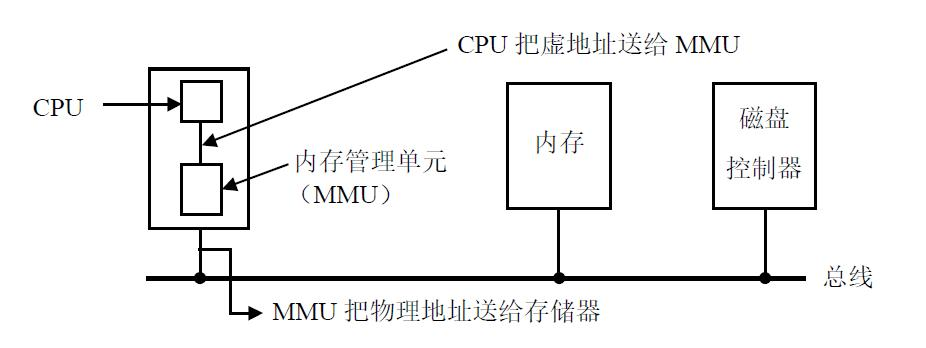
\includegraphics[width=12cm]{lab2-mmu}
  \caption{MMU的位置和功能}\label{lab2-mmu}
\end{figure}

我们所熟悉的查询二级页表访存机制,即先查询页目录,再查询相应的二级页表的工作,都是由MMU来完成的。

\subsection{TLB}

我们知道,访存效率在体系结构的设计中是一个很重要的问题,但我们应用的页表机制却会降低系统的性能,举例来说,如果没有页表,那么只需要一次访存,但如果有了二级页表,就需要三次访存。虽然页表机制能带来许多好处,但是这样降低效率还是无法让人接受的,为了解决这一问题,我们需要一个能让计算机能够不经过页表就把虚拟地址映射成物理地址的硬件设备,这就是TLB。

TLB的全称是Translation Lookside Buffer,中文为翻译后援存储器,有的时候也叫相联存储器(Associative Memory),或者快表,它通常被安装在MMU的内部,如下图\ref{lab2-tlb}所示:

\begin{figure}[htbp]
  \centering
  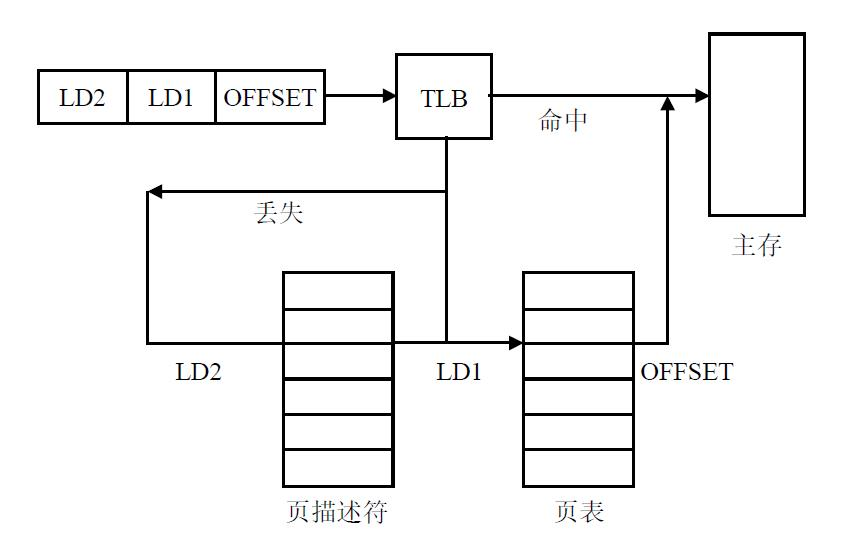
\includegraphics[width=12cm]{lab2-tlb}
  \caption{TLB示意图}\label{lab2-tlb}
\end{figure}

简单来说,TLB就是页表的高速缓存,每个TLB的条目中包含有一个页面的所有信息(有效位、虚页号、物理页号、修改位、保护位等等),这些条目中的内容和页表中相同页面的条目中的内容是完全一致的。

当一个虚拟地址被送到MMU中进行翻译的时候,硬件首先在TLB中寻找包含这个地址的页面,如果它的虚页号在TLB中,并且没有违反保护位,那么就可以直接从TLB中得到相应的物理页号,而不去访问页表;如果发现虚页号在TLB中不存在,那么MMU将进行常规的页表查找,同时通过一定的策略来将这一页的页表项替换到TLB中,之后再次访问这一页的时候就可以直接在TLB中找到。

容易发现,如果TLB命中,那么我们只需要访问两次内存就可以得到需要的数据,从而从整体上降低了平均访存时间。

到此为止,我们已经基本了解了内存访问的机制。

\subsection{内存访问}

在这之前,我们一直忽略了访存的一个重要部件————cache,相信你已经多次在课堂上接触过这个概念,计算机中的访存过程中一定存在着和cache相关的过程,而之前对cache的忽略就意味着我们对内存访问机制的了解是不全面的,这就产生了下面的三个问题:

\begin{enumerate}
  \item TLB、cache、MMU、页表这些东西之间有什么关系?
  \item 一个完整的访存流程是怎样的?
  \item 我们在这次实验中要完成的内存管理在这个流程中起了什么作用?
\end{enumerate}

这一节中我们将分别回答这些问题,在你往下看之前,也许你可以先思考一下这些问题,看看下面给出的解答是否符合你的预期。

接下来的讲解将会涉及到cache中的一些概念,我们假设你对这些概念都有一定的了解,如果你感觉有些不确定或者忘了这些内容,你可以回头翻翻计组课本中的相关内容。

一般来说,cache中用来查询相应地址是否存在时所用的地址是物理地址的一部分,这就是cache中的tag,如果是这样,那么很自然的,访存时候所用的虚拟地址应该首先经过TLB和MMU转换成物理地址,然后在cache中查找是否命中,基于这样的考虑,那么完整的访存流程应该是这样的:

\begin{enumerate}
  \item CPU给出虚拟地址来访问数据,TLB接收到这个地址之后查找是否有对应的页表项。
  \item 假设页表项存在,则根据物理地址在cache中查询;如果不存在,则MMU执行正常的页表查询工作之后再根据物理地址在cache中查询,同时更新TLB中的内容。
  \item 如果cache命中,则直接返回给CPU数据;如果没有命中则按照相应的算法进行cache的替换或者装填,之后返回给CPU数据。
\end{enumerate}

看上去上面的访存过程没什么问题,但如果上述过程是按顺序执行的,那么自然就产生了问题,每次访存都需要先经过TLB,如果TLB命中还能接受,可如果TLB没有命中,同时这个地址又恰好在cache中存在,那么这种情况下先将地址经过MMU翻译再在cache中查询岂不是会造成性能上的损失?

我们把这个问题留给你来思考。

\begin{thinking}\label{think-cache}
  请思考cache用虚拟地址来查询的可能性,并且给出这种方式对访存带来的好处和坏处。另外,你能否能根据前一个问题的解答来得出用物理地址来查询的优势?
\end{thinking}

虽然提出了相应的疑问,但是我们可以认为上述过程是大致正确的,当然,这里还有一个问题留给你思考。

\begin{thinking}\label{think-memory-access}
  请查阅相关资料,针对我们提出的疑问,给出一个上述流程的优化版本,新的版本需要有更快的访存效率。(提示:考虑并行执行某些步骤)
\end{thinking}

到此,我们已经解决了前面提出的前两个问题。

回想前面的访存过程我们可以发现有一个过程是我们没有提到的,即页表内容的填充。虽然MMU可以自动访问页表得到虚拟地址相应的物理地址,但如果只有一个空荡荡的页表,那么MMU是无法工作的;同时,操作系统需要在软件层面上对内存进行管理和控制,以便为上层的应用提供相应的接口。我们这次的实验就是围绕着这些内容来展开的。

\section{MIPS虚存映射布局}

32位的MIPS CPU最大寻址空间为4GB(2\^{}32字节),这4GB虚存空间被划分为四个部分:

\begin{enumerate}
  \item kuseg (TLB-mapped cacheable user space, 0x00000000 $\scriptsize{\sim}$ 0x7f\/f\/f\/f\/f\/f\/f):
  这一段是用户模式下可用的地址,大小为2G,也就是MIPS约定的用户内存空间。需要通过MMU进行虚拟地址到物理
  地址的转换。
  \item kseg0 (direct-mapped cached kernel space, 0x80000000 $\scriptsize{\sim}$ 0x9f\/f\/f\/f\/f\/f\/f):
  这一段是内核地址,其内存虚存地址到物理内存地址的映射转换不通过MMU,使用时只需要将地址的最高位清零
  (\& 0x7f\/f\/f\/f\/f\/f\/f),
  这些地址就被转换为物理地址。也就是说,这段逻辑地址被连续地映射到物理内存的低端512M空间。对这段地址
  的存取都会通过高速缓存(cached)。通常在没有MMU的系统中,这段空间用于存放大多数程序和数据。对于有
  MMU 的系统,操作系统的内核会存放在这个区域。
  \item kseg1 (direct-mapped uncached kernel space, 0xa0000000 $\scriptsize{\sim}$ 0xbf\/f\/f\/f\/f\/f\/f):
  与kseg0类似,这段地址也是内核地址,将虚拟地址的高 3 位清零(\& 0x1f\/f\/f\/f\/f\/f\/f),就可以转换到物理地址,
  这段逻辑地址也是被连续地映射到物理内存的低端512M空间。但是 kseg1 不使用缓存(uncached),访问速度比较慢,
  但对硬件I/O寄存器来说,也就不存在Cache一致性的问题了,这段内存通常被映射到I/O寄存器,用来实现对外设的访问。
  \item kseg2 (TLB-mapped cacheable kernel space, 0xc0000000 $\scriptsize{\sim}$ 0xf\/f\/f\/f\/f\/f\/f\/f):
  这段地址只能在内核态下使用,并且需要 MMU 的转换。
\end{enumerate}

\section{内存管理与内存翻译}

  内存管理的实质是为每个程序提供自己的内存空间。最为朴素的内存管理就是直接将物理内存分配给程序,一个萝卜一个坑。
  但从之前的叙述中,我们可以发现,MIPS系统中,使用了虚拟内存的技术。因此在我们的系统中,同时存在着两套地址,
  一套是真实的物理地址,另一套则是虚拟地址,这为我们的内存管理带来了许多内存翻译的工作。这些工作大多就是由
  前文所述的MMU来完成。
  为什么我们要这么做呢?原因有很多:
    \begin{enumerate}
      \item 隐藏与保护:因为加入了虚拟内存这一中间层,真实的物理地址对用户级程序是不可见的,它只能访问
      操作系统允许其访问的内存区域。
      \item 为程序分配连续的内存空间:利用虚拟内存,操作系统可以从物理分散的内存页中,构建连续的程序空间,
      这使得我们拥有更高的内存利用率。
      \item 扩展地址空间范围:如前文所述,通过虚拟内存,MIPS32位机拥有了4GB的寻址能力,这真的很cool。:)
      \item 使内存映射适合你的程序:在大型操作系统中,可能存在相同程序的多个副本同时运行,这时候通过内存翻译
      这一中间层,你能使他们都使用相同的程序地址,这让很多工作都简单了很多。
      \item 重定位:程序入口地址和预先声明的数据在程序编译的过程中就确定了。但通过MMU的内存翻译,我们能够让程
      序运行在内存中的任何位置。
    \end{enumerate}
  为了这些好处,我们需要付出地址翻译工作的代价。接下来我们在lab的工作中,也将一直遇到这个问题。建议各位在lab的
  过程中,不妨思考当前我们使用的这个地址究竟是物理地址还是虚拟地址,搞清楚这一点,对我们的lab和操作系统的理解都
  大有帮助。

\section{物理内存管理}

\subsection{初始化流程说明}
  在第一个实验中,我们将内核加载到内存中的 kseg0 区域(0x80010000),成功启动并跳转到 init/main.c 中的
   main 函数开始运行,现在我们需要在 main 函数中调用定义在 init/init.c 中的 mips\_init() 函数,并
  进一步通过

  \begin{enumerate}
    \item \mintinline{c}|mips_detect_memory()|;
    \item \mintinline{c}|mips_vm_init()|;
    \item \mintinline{c}|page_init()|;
  \end{enumerate}

  这三个函数来实现物理内存管理的相关数据结构的初始化。

\subsection{内存控制块}

在MIPS CPU 中,地址转换以4KB 大小为单位,称为页。整个物理内存按4KB大小分成了许多页,我们大多数时候的
内存分配,也是以页为单位来进行。为了记录分配情况,我们需要使用 Page 结构体来记录一页内存的相关信息:

\begin{minted}[linenos]{c}
typedef LIST_ENTRY(Page) Page_LIST_entry_t;

struct Page {
    Page_LIST_entry_t pp_link;  /* free list link */
    u_short pp_ref;
};
\end{minted}

其中,\mintinline{c}|pp_ref| 用来记录这一物理页面的引用次数,\mintinline{c}|pp_link| 是当前节点
指向链表中下一个节点的指针,其类型为 \mintinline{c}|LIST_ENTRY(Page)| 。我们在 include/queue.h
中定义了一系列的宏函数来简化对链表的操作。请阅读这些宏函数的代码,理解它们的原理和巧妙之处。

\begin{thinking}\label{think-do_while}
我们注意到我们把宏函数的函数体写成了 \mintinline{c}|do { /* ... */ } while(0)| 的形式,而不是
仅仅写成形如
\mintinline{c}|{ /* ... */ }| 的语句块,这样的写法好处是什么?
\end{thinking}

在 include/pmap.h 中,我们使用 LIST\_HEAD 宏来定义了一个结构体类型 Page\_list ,在 mm/pmap.c
中,创建了一个该类型的变量 page\_free\_list 来以链表的形式表示所有的空闲物理内存:

\begin{minted}[linenos]{c}
LIST_HEAD(Page_list, Page);

static struct Page_list page_free_list; /* Free list of physical pages */
\end{minted}

\begin{thinking}\label{think-struct-page}
注意,我们定义的 Page 结构体只是一个信息的载体,它只代表了相应物理内存页的信息,它本身并不是物理内存页。
那我们的物理内存页究竟在哪呢?Page 结构体又是通过怎样的方式找到它代表的物理内存页的地址呢?
请你阅读 include/pmap.h 与 mm/pmap.c 中相关代码,给出你的想法。
\end{thinking}

\subsection{内存分配和释放}

首先,我们需要注意在 mm/pmap.c 中定义的与内存相关的全局变量:

\begin{minted}[linenos]{c}
u_long maxpa;            /* Maximum physical address */
u_long npage;            /* Amount of memory(in pages) */
u_long basemem;          /* Amount of base memory(in bytes) */
u_long extmem;           /* Amount of extended memory(in bytes) */
\end{minted}

\begin{exercise}
我们需要在 mips\_detect\_memory() 函数中初始化这几个全局变量,以确定内核可用的物理内存的大小和范围。
根据代码注释中的提示,完成 mips\_detect\_memory() 函数。
\end{exercise}

在操作系统刚刚启动时,我们还没有建立起有效的数据结构来管理所有的物理内存,因此,出于最基本的
内存管理的需求,我们需要实现一个函数来分配指定字节的物理内存。这一功能由 mm/pmap.c 中的
alloc函数来实现。

\begin{minted}[linenos]{c}
static void *alloc(u_int n, u_int align, int clear);
\end{minted}

alloc 函数能够按照参数 align 进行对齐,然后分配 n 字节大小的物理内存,并根据参数 clear 的设定决
定是否将新分配的内存全部清零,并最终返回新分配的内存的首地址。

\begin{thinking}\label{think-bzero}
在 mmu.h 中定义了\mintinline{c}|bzero(void *b, size_t)|这样一个函数,请你思考,此处的b指针是一个物理地址,
还是一个虚拟地址呢?
\end{thinking}

有了分配物理内存的功能后,接下来我们需要给操作系统内核必须的数据结构 -- 页目录(pgdir)、内存控制块
数组(pages)和进程控制块数组(envs)分配所需的物理内存。mips\_vm\_init() 函数实现了这一功能,
并且完成了相关的虚拟内存与物理内存之间的映射。

完成上述工作后,我们便可以通过在 mips\_init() 函数中调用 page\_init() 函数将余下的物理内存块加
入到空闲链表中。

\begin{exercise}
完成 page\_init 函数,使用 include/queue.h 中定义的宏函数将未分配的物理页加入到空闲链表
page\_free\_list 中去。思考如何区分已分配的内存块和未分配的内存块,并注意内核可用的物理内存上限。
\end{exercise}

有了记录物理内存使用情况的链表之后,我们就可以不再像之前的 alloc 函数那样按字节为单位进行内存
的分配,而是可以以页为单位 进行物理内存的分配与释放。page\_alloc 函数用来从空闲链表中分配一页
物理内存,而 page\_free 函数则用于将一页之前分配的内存重新加入到空闲链表中。

\begin{exercise}
完成 mm/pmap.c 中的 page\_alloc 和 page\_free 函数,基于空闲内存链表 page\_free\_list ,以页
	为单位进行物理内存的管理。并在init/init.c的函数mips\_init中注释掉page\_check();。此时运行结果如下。
\end{exercise}

\begin{minted}[linenos]{c}
main.c: main is start ...
init.c: mips_init() is called
Physical memory: 65536K available, base = 65536K, extended = 0K
to memory 80401000 for struct page directory.
to memory 80431000 for struct Pages.
pmap.c:  mips vm init success
*temp is 1000
phycial_memory_manage_check() succeeded
panic at init.c:17: ^^^^^^^^^^^^^^^^^^^^^^^^^^^^^^^^^^^^^
\end{minted}


至此,我们的内核已经能够按照分页的方式对物理内存进行管理,

\section{虚拟内存管理}

我们通过建立两级页表来进行虚拟内存的管理,在此基础上,我们将实现根据虚拟地址在页表中查找
对应的物理地址,以及将一段虚存地址映射到一段的物理地址的功能,然后实现虚存的管理与释放,最后为内核建立起一
套虚存管理系统。

\subsection{两级页表机制}

我们的操作系统内核采取二级页表结构,如图\ref{lab2-pic-1}所示:

\begin{figure}[htbp]
  \centering
  \includegraphics[width=12cm]{lab2-pic-1}
  \caption{二级页表结构示意图}\label{lab2-pic-1}
\end{figure}

第一级表称为页目录(page directory),一共1024个页目录项,每个页目录项32位(4 Byte),页目录项存储
的值为其对应的二级页表入口的物理地址。整个页目录存放在一个页面(4KB)中,也就是我们在 mips\_vm\_init
函数中为其分配了相应的物理内存。第二级表称为页表(page table),每一张页表有1024个页表项,每个页表
项32位(4 Byte),页表项存储的是对应页面的页框号(20位)以及标志位(12位)。每张页表占用一个页面大小
(4KB)的内存空间。

对于一个32位的虚存地址,其31-22位表示的是页目录项的索引,21-12位表示的是页表项的索引,11-0位表示的
是该地址在该页面内的偏移。

\subsection{地址转换}

对于操作系统来说,虚拟地址与物理地址之间的转换是内存管理中非常重要的内容。在这一部分,我们将详细探讨
咱们的内核是如何进行地址转换的。

首先从较为简单的形式开始。在前面的实验中,我们通过设置 lds 文件让操作系统内核加载到内存的 0x80010000
位置,在上文我们对 MIPS 存储器映射布局的介绍中我们知道,这一地址对应的是 kseg0 区域,这一部分的地址
转换不通过 MMU 进行。我们也称这一部分虚拟地址为内核虚拟地址。从虚拟地址到物理地址的转换只需要清掉
最高位的零即可,反过来,将对应范围内的物理地址转换到内核虚拟地址,也只需要将最高位设置为1即可。我们在
 include/mmu.h 中定义了 PADDR 和 KADDR 两个宏来实验这一功能:

\begin{minted}[linenos]{c}
// translates from kernel virtual address to physical address.
#define PADDR(kva)            \
  ({                \
    u_long a = (u_long) (kva);        \
    if (a < ULIM)         \
      panic("PADDR called with invalid kva %08lx", a);\
    a - ULIM;           \
  })

// translates from physical address to kernel virtual address.
#define KADDR(pa)           \
  ({                \
    u_long ppn = PPN(pa);         \
    if (ppn >= npage)         \
      panic("KADDR called with invalid pa %08lx", (u_long)pa);\
    (pa) + ULIM;          \
  })
\end{minted}

在 PADDR 中,我们使用了一个宏 ULIM ,这个宏定义在 include/mmu.h 中,其值为 0x80000000。对于小于
 0x80000000 的虚拟地址值,显然不可能是内核区域的虚拟地址。在 KADDR 中,一个合理的物理地址的物理
页框号显然不能大于我们在 mm/pmap.c 中所定义的物理内存总页数 npage 的值。

接下来,我们讨论如何通过二级页表进行虚拟地址到物理地址的转换。

首先,我们可以通过 PDX(va) 来获得一个虚拟地址对应的页目录索引,然后直接凭借索引在页目录中得到对应的
二级页表的基址(物理地址),然后把这个物理地址转化为内核虚拟地址(KADDR),之后,通过 PTX(va) 获得这个
虚存地址对应的页表索引,然后就可以从页表中得到对应的页面的物理地址。整个转换的过程如 图\ref{lab2-pic-2}
所示:

\begin{figure}[htbp]
  \centering
  \includegraphics[width=12cm]{lab2-pic-2}
  \caption{地址转换过程}\label{lab2-pic-2}
\end{figure}

\subsection{页目录自映射}

上文中我们讲二级页表结构的时侯提到,要映射整个4G地址空间,一共需要1024个页表和1个页目录的。一个页表占用 4KB
空间,页目录也占用 4KB 空间,也就是说,整个二级页表结构将占用 4MB+4KB 的存储空间,1024*4KB+1*4KB=4MB+4KB。

在 include/mmu.h 中的内存布局图里有这样的内容:

\begin{minted}[linenos]{c}
/**
 *      ULIM     -----> +----------------------------+------------0x8000 0000-------
 *                      |         User VPT           |     PDMAP                /|\
 *      UVPT     -----> +----------------------------+------------0x7fc0 0000    |
 */
\end{minted}

不难计算出 UVPT(0x7fc00000) 到 ULIM(0x80000000) 之间的空间只有 4MB ,这一区域就是进程的
页表的位置,于是我们不禁想问:页目录所占用的 4KB 内存空间在哪儿?

\textbf{答案就在于页目录的自映射机制!}

如果页表和页目录没有被映射到进程的地址空间中,而一个进程的4GB地址空间又都映射了物理内存的话,那么就确实需要
1024个物理页(4MB)来存放页表,和另外1个物理页(4KB)来存放页目录,也就是需要(4M+4K)的物理内存。但是页表也被映射
到了进程的地址空间中,也就意味着 1024 个页表中,有一个页表所对应的 4M 空间正是这 1024 个页表所占用的 4M 内存,
这个页表的 1024 的页表项存储了 1024 个物理地址,分别是 1024 个页表的物理地址。而在二级页表结构中,页目录
对应着二级页表,1024 个页目录项存储的也是全部 1024 个页表的物理地址。也就是说,一个页表的内容和页目录的
内容是完全一样的,正是这种完全相同,使得将 1024 个页表加 1 个页目录映射到地址空间只需要 4M 的地址空间,
\textbf{其中的一个页表和页目录完全重合了}。

接下来我们会想到这样一个问题:那么,这个与页目录重合的页表,也就是页目录究竟在哪儿呢?

我们知道,这 4M 空间的起始位置也就是第一个二级页表对应着页目录的第一个页目录项,同时,由于 1M 个页表项和 4G
地址空间是线性映射,不难算出 0x7fc00000 这一地址对应的应该是第 (0x7fc00000 \verb|>>| 12) 个页表项,这个页表项
也就是第一个页目录项。一个页表项 32 位,占用 4 个字节的内存,因此,其相对于页表起始地址 0x7fc000000 的
偏移为 (0x7fc00000 \verb|>>| 12) * 4 = 0x1f\/f000 ,于是得到地址为 0x7fc00000 + 0x1f\/f000 = 0x7fdf\/f000 。也就是
说,页目录的虚存地址为 0x7fdf\/f000。

\begin{thinking}\label{think-windows_pde_addr}
了解了二级页表页目录自映射的原理之后,我们知道,Win2k内核的虚存管理也是采用了二级页表的形式,其页表所占的 4M
空间对应的虚存起始地址为 0xC0000000,那么,它的页目录的起始地址是多少呢?
\end{thinking}

\subsection{创建页表}

将虚拟地址转换为物理地址的过程中,如果这个虚拟地址所对应的二级页表不存在,有时,我们可能需要为这个
虚拟地址创建一个新的页表。我们需要申请一页物理内存来存放这个页表,然后将他的物理地址赋值给对应的页
目录项,最后设置好页目录项的权限位即可。

我们的内核在 mm/pmap.c 中分定义了 boot\_pgdir\_walk 和 pgdir\_walk 两个函数来实现地址转换和
页表的创建,这两个函数的区别仅仅在于当虚存地址所对应的页表的页面不存在的时候,分配策略的不同和使用的
内存分配函数的不同。前者用于内核刚刚启动的时候,这一部分内存通常用于存放内存控制块和进程控制块等数据
结构,相关的页表和内存映射必须建立,否则操作系统内核无法正常执行后续的工作。然而用户程序的内存
申请却不是必须满足的,当可用的物理内存不足时,内存分配允许出现错误。boot\_pgdir\_walk 被调用时,
还没有建立起空闲链表来管理物理内存,因此,直接使用 alloc 函数以字节为单位进行物理内存的分配,而
 pgdir\_walk 则在空闲链表初始化之后发挥功能,因此,直接使用 page\_alloc 函数从空闲链表中
以页为单位进行内存的申请。

上文中介绍了页目录自映射的相关知识,我们了解到页目录其实也是一个页表。我们知道,在咱们实验使用的内核中,
一个页表指向的物理页面存在的标志是页表项存储的值的 PTE\_V 标志位被置为 1 。因此,在将页表的物理地址赋值
给 页目录项时,我们还为页目录项设置权限位。

\begin{exercise}
完成 mm/pmap.c 中的 boot\_pgdir\_walk 和 pgdir\_walk 函数,实现虚拟地址到物理地址的转换以及创建页表的功能。
\end{exercise}

\subsection{地址映射}
一个空荡荡的页表自然不会对我们的内存翻译有帮助,我们需要在具体的物理内存与虚拟地址间建立映射,即将相应的物理页面地址填入对应虚拟地址的页表项中。
\begin{exercise}
实现 mm/pmap.c 中的 boot\_map\_segment 函数,实现将制定的物理内存与虚拟内存建立起映射的功能。
\end{exercise}

\subsection{page insert and page remove}

\begin{minted}[linenos]{c}
// Overview:
//   Map the physical page 'pp' at virtual address 'va'.
//   The permissions (the low 12 bits) of the page table entry
//   should be set to 'perm|PTE_V'.
//
// Post-Condition:
//   Return 0 on success
//   Return -E_NO_MEM, if page table couldn't be allocated
//
// Hint:
//   If there is already a page mapped at `va`, call page_remove()
//   to release this mapping.The `pp_ref` should be incremented
//   if the insertion succeeds.
int
page_insert(Pde *pgdir, struct Page *pp, u_long va, u_int perm)
{
	u_int PERM;
	Pte *pgtable_entry;
	PERM = perm | PTE_V;

	/* Step 1: Get corresponding page table entry. */
	pgdir_walk(pgdir, va, 0, &pgtable_entry);

	if (pgtable_entry != 0 && (*pgtable_entry & PTE_V) != 0) {
		if (pa2page(*pgtable_entry) != pp) {
			page_remove(pgdir, va);
		}
		else{
			tlb_invalidate(pgdir, va);
			*pgtable_entry = (page2pa(pp) | PERM);
			return 0;
		}
	}

	/* Step 2: Update TLB. */
	tlb_invalidate(pgdir, va);

	/* Step 3: Do check, re-get page table entry to validate
	 *  the insertion. */
	if (pgdir_walk(pgdir, va, 1, &pgtable_entry) != 0) {
		return -E_NO_MEM;    // panic ("page insert failed .\n");
	}

	*pgtable_entry = (page2pa(pp) | PERM);
	pp->pp_ref++;
	return 0;
}
\end{minted}

这个函数虽然我们并没有填,但是\textbf{非常重要}!这个函数将在\textbf{lab3和lab4}中被反复用到,这个函数
将va虚拟地址和其要对应的物理页pp的映射关系以perm的权限设置加入页目录。我们大概讲一下函数的执行流程与执行要点。

\textbf{流程大致如下:}先判断va是否有对应的页表项:如果页表项有效(或者叫va是否已经有了映射的物理地址)
的话,则去判断这个物理地址是不是我们要插入的那个物理地址,如果不是,那么就把该物理地址移除掉;
如果是的话,则修改权限,放到tlb中。

\textbf{有一个值得指出的要点}:我们能看到,只要对页表的内容修改,都必须tlb\_invalidate 来让tlb更新,否则后面紧接着对内存的访问很有可能出错。

可以说tlb\_invalidate 函数是它的一个核心子函数,这个函数实际上又是由tlb\_out 汇编函数组成的。

\begin{codeBoxWithCaption}{TLB汇编函数\label{code:tlb_out.S}}
  \inputminted[linenos]{gas}{codes/tlb_out.S}
\end{codeBoxWithCaption}

这个汇编函数相对其他汇编函数来说相对简单,那么留给你一个思考问题.

\begin{thinking}\label{think-tlb}
思考一下tlb\_out 汇编函数,结合代码阐述一下跳转到\textbf{NOFOUND}的流程?
\end{thinking}
\subsection{访存与TLB重填}
  通过之前的实验,我们可以知道,虚拟地址通过MMU转换成物理地址,然后通过物理地址我们能够在主存中获得相应的数据。而实际上,在MIPS架构中,关于这一块
  内存翻译的内容,很大程度上与TLB有关。TLB可以看做是一块页表的高速缓存,里面存储了一些物理页面与虚拟页面的对应关系。而当CPU访问相应内存地址时,会先去
  TLB中查询。当TLB中没有相应对应关系时会触发一个\textbf{TLB缺失异常}。而MIPS将这个异常的处理,全权交给了软件。因此若发生缺失异常,则会跳转到相应异常处理程序中,
  再由我们的二级页表进行相应的地址翻译,对TLB进行重填。换句话说,MIPS中并没有一个执行内存地址翻译的MMU处理器,CPU完成了相应工作。

  如果大家仔细地理解了上面这段话,就会发现MMU的正常工作需要\textbf{异常处理}的支持。由于我们暂时还不了解异常的相关内容,因此在本次实验中实际上并没有真正地启用MMU,而只是先创建了页表。
  在lab3中学习完中断和异常后,我们就能够见到一个真正启用的MMU了。

  而现在,为了深究整个过程,让我们来一起探索一个假设情境:在page\_check最后一句printf之前添加如下代码段。
  提醒一下,由于MMU暂时没有启用,这段代码目前不能在我们的系统中实际运行:

  \begin{minted}[linenos]{c}
    u_long* va = 0x12450;
    u_long* pa;

    page_insert(boot_pgdir, pp, va, PTE_R);
    pa = va2pa(boot_pgdir, va);
    printf("va: %x -> pa: %x\n", va, pa);
    *va = 0x88888;
    printf("va value: %x\n", *va);
    printf("pa value: %x\n", *((u_long *)((u_long)pa + (u_long)ULIM)));
  \end{minted}

  这段代码旨在计算出相应va与pa的对应关系,设置权限位为PTE\_R是为了能够将数据写入内存。

  如果MMU能够正常工作,实际输出将会是:

  \begin{minted}[linenos]{c}
    va: 12450 -> pa: 3ffd000
    va value: 88888
    pa value: 0
    page_check() succeeded!
  \end{minted}

  \begin{thinking}\label{think-memory-access}
  显然,运行后结果与我们预期的不符,va值为0x88888,相应的pa中的值为0。这说明我们的代码中存在问题,请你仔细思考我们的访存模型,指出问题所在。
  \end{thinking}
  另外,还可以提醒大家的是,在gxemul中,有tlbdump这个命令,可以随时查看tlb中的内容。
\section{正确结果展示}

实验二做完之后,在init/init.c的函数mips\_init中,将page\_check还原,并注释掉physical\_memory\_manage\_check();。运行的正确结果应该是这样的:

\begin{minted}[linenos]{c}
main.c: main is start ...
init.c: mips_init() is called
Physical memory: 65536K available, base = 65536K, extended = 0K
to memory 80401000 for struct page directory.
to memory 80431000 for struct Pages.
mips_vm_init:boot_pgdir is 80400000
pmap.c:  mips vm init success
start page_insert
va2pa(boot_pgdir, 0x0) is 3ffe000
page2pa(pp1) is 3ffe000
pp2->pp_ref 0
end page_insert
page_check() succeeded!
panic at init.c:55: ^^^^^^^^^^^^^^^^^^^^^^^^^^^^^^^^^^^^^
\end{minted}

地址\textbf{3ffe000}和最后一行的数字 \textbf{55} 是不固定的。

\section{实验思考}

\begin{itemize}
\item \hyperref[think-cache]{\textbf{\textcolor{baseB}{思考-不同地址类型查询cache的比较}}}
\item \hyperref[think-memory-access]{\textbf{\textcolor{baseB}{思考-优化访存过程}}}
\item \hyperref[think-do_while]{\textbf{\textcolor{baseB}{思考-使用do-while(0)语句的好处}}}
\item \hyperref[think-struct-page]{\textbf{\textcolor{baseB}{思考-Page结构体与物理内存页}}}
\item \hyperref[think-bzero]{\textbf{\textcolor{baseB}{思考-bzero参数探究}}}
\item \hyperref[think-windows_pde_addr]{\textbf{\textcolor{baseB}{思考-自映射机制页目录地址的计算}}}
\item \hyperref[think-tlb]{\textbf{\textcolor{baseB}{思考-NOFOUND的奥妙}}}
\item \hyperref[think-memory-access]{\textbf{\textcolor{baseB}{思考-访存的问题}}}
\end{itemize}

\section{挑战性任务——Buddy System}

在这次实验中,我们建立了一个简单的页式内存管理系统,你可能已经对操作系统如何控制内存有了初步的了解,但是为了更进一步了解现代操作系统,这还远远不够。现代操作系统为了追求高效的内存管理,使用了很多复杂的技术,在这次挑战性任务中,你将通过探究并实现一个现在在Linux中仍然被广泛使用的物理内存管理算法——伙伴系统,来深入了解内存管理中的问题和相关技术。


\subsection{Buddy System}

伙伴系统(Buddy System)是一种支持分配大量连续页面,并能有效减少内存中外碎片的物理内存分配管理算法。相信大家通过“操作系统”理论课的学习,已经对这个算法有了初步的认识,在这里我们只说明减少内存中碎片的必要性,以及对伙伴系统的一些不同版本进行一些简单介绍,而对算法的进一步探究和实现将完全交给同学们来完成。

所谓内存中的外碎片就是指那些还没有分配出去,但是因为空间太小不足以分配给新进程的内存空闲区域,这种碎片一般处于两块已经分配出去的内存的中间。外碎片的增多带来的问题就是,虽然所有碎片加起来的空间可以满足一些请求的空间要求,但当请求需要分配大块连续页面则不能满足。

我们现在使用的按页分配空间的算法,很容易产生很多外碎片,这时就需要像伙伴系统这样的算法来控制外碎片的数量。

Linux中使用伙伴系统来管理物理内存,并且从Linux 2.6.32开始,通过引入迁移类型(Migrate Type)进一步优化了伙伴系统,但在这里你不需要考虑这个改进。

\subsection{题目要求}
在lab2或者lab2之后的实验的分支中,新建lab2-challenge分支。

在lab2代码的基础上,实现一个伙伴系统,需要实现的功能包括:

\begin{enumerate}
  \item 根据伙伴算法,使得系统可以分配4MB(或者更大)的连续内存
  \item 根据伙伴算法来释放内存,尽可能地合并伙伴
  \item 记录空闲的大小为2\^{}n(n=0,1,2...MAX,MAX是你设定的值)页内存块的个数
  \item 实现一个类似page\_check()的函数,证明你所实现的系统的正确性
\end{enumerate}

下面是一个可能的分配、释放内存接口的例子

\begin{minted}[linenos]{c}
void pages_alloc(struct Page **pp, unsigned int order);
void pages_free(struct Page *pp, unsigned int order);
\end{minted}

其中第二个参数order表示需要分配(释放)2\^{}order页的内存,第一个参数**pp(*pp)是这个内存块的第一页。

完成之后提交到同名的远程分支即可。
\chapter{进程与异常}

\section{实验目的}
  \begin{enumerate}
    \item 创建一个进程并成功运行
    \item 实现时钟中断,通过时钟中断内核可以再次获得执行权
    \item 实现进程调度,创建两个进程,并且通过时钟中断切换进程执行
  \end{enumerate}

在本次实验中你将运行一个用户模式的进程。你需要使用数据结构进程控制块 Env 来跟踪用户进程。
通过建立一个简单的用户进程,加载一个程序镜像到进程控制块中,并让它运行起来。
同时,你的MIPS内核将拥有处理异常的能力。

\section{进程}

\begin{note}
进程既是基本的分配单元,也是基本的执行单元。第一,进程是一个实体。每一个进程都有它自己的地址空间,
一般情况下,包括代码段、数据段和堆栈。第二,进程是一个“执行中的程序”。
程序是一个没有生命的实体,只有处理器赋予程序生命时,它才能成为一个活动的实体,我们称其为进程。
\end{note}

\subsection{进程控制块}

这次实验是关于进程和异常的,那么我们首先来结合代码看看进程控制块是个什么东西。

进程控制块(PCB)是系统为了管理进程设置的一个专门的数据结构,用它来记录进程的外部特征,描述进程的运动变化过程。
系统利用PCB来控制和管理进程,所以\textbf{PCB是系统感知进程存在的唯一标志。进程与PCB是一一对应的。}
通常PCB应包含如下一些信息:

\begin{codeBoxWithCaption}{进程控制块\label{code:process_of_env.h}}
  \inputminted[linenos]{c}{codes/process_of_env.h}
\end{codeBoxWithCaption}

为了集中你的注意力在关键的地方,我们暂时不介绍其他实验所需介绍的内容。
下面是\textbf{lab3}中需要用到的这些域的一些简单说明:

\begin{itemize}
  \item env\_tf : Trapframe 结构体的定义在\textbf{include/trap.h} 中,env\_tf 的作用就是在进程因为时间片用光不再运行时,将其当时的进程上下文环境保存在env\_tf 变量中。当从用户模式切换到内核模式时,内核也会保存进程上下文,因此进程返回时上下文可以从中恢复。
  \item env\_link : env\_link 的机制类似于实验二中的 pp\_link,使用它和 env\_free\_list 来构造空闲进程链表。
  \item env\_id : 每个进程的 env\_id 都不一样,env\_id 是进程独一无二的标识符。
  \item env\_parent\_id : 该变量存储了创建本进程的进程 id。
  这样进程之间通过父子进程之间的关联可以形成一颗进程树。
  \item env\_status : 该变量只能在以下三个值中进行取值:
  \begin{itemize}
    \item ENV\_FREE : 表明该进程是不活动的,即该进程控制块处于进程空闲链表中。
    \item ENV\_NOT\_RUNNABLE : 表明该进程处于阻塞状态,
    处于该状态的进程往往在等待一定的条件才可以变为就绪状态从而被CPU调度。
    \item ENV\_RUNNABLE : 表明该进程处于就绪状态,正在等待被调度,
    但处于RUNNABLE状态的进程可以是正在运行的,也可能不在运行中。
  \end{itemize}
  \item env\_pgdir : 这个变量保存了该进程页目录的虚拟地址。
  \item env\_cr3 : 这个变量保存了该进程页目录的物理地址。
  \item env\_sched\_link : 这个变量来构造就绪状态进程链表。
  \item env\_pri :  这个变量保存了该进程的优先级。
\end{itemize}

这里值得强调的一点就是\textbf{ENV\_RUNNABLE 状态并不代表进程一定在运行中,它也可能正处于调度队列中}。
而我们的进程调度也只会调度处于RUNNABLE状态的进程。

既然我们知道了进程控制块,我们就来认识一下进程控制块数组\textbf{envs}。在我们的实验中,
存放进程控制块的物理内存在系统启动后就要被分配好,并且这块内存不可被换出。
所以需要在系统启动后就要为envs数组分配内存,下面你就要完成这个重任

\begin{exercise}
  \begin{itemize}
    \item 修改pmap.c/mips\_vm\_init函数来为envs数组分配空间。
    \item envs数组包含 NENV 个Env结构体成员,你可以参考pmap.c中已经写过的\textbf{pages}数组空间的分配方式。
    \item 除了要为数组 envs 分配空间外,你还需要使用 pmap.c 中你填写过的一个内核态函数为其进行段映射,
    envs 数组应该被\textbf{UENVS}区域映射,你可以参考\textbf{./include/mmu.h}。	
  \end{itemize}
\end{exercise}

当然我们光有了存储进程控制块信息的envs还不够,我们还需要像lab2一样将空闲的env控制块按照链表形式“串”起来,便于后续分配ENV结构体对象,形成env\_free\_list。一开始我们的所有进程控制块都是空闲的,所以我们要把它们都“串”到env\_free\_list上去。

\begin{exercise}
仔细阅读注释,填写\textbf{env\_init}函数,注意链表插入的顺序(函数位于lib/env.c中)。
\end{exercise}

在填写完env\_init函数后,我们对于envs的操作暂时就告一段落了,不过我们还有一个小问题没解决,为什么严格规定链表的插入顺序?我们需要你来仔细思考,注释中已经给出了提示。

\begin{thinking}\label{think-env_init}
    为什么我们在构造空闲进程链表时必须使用特定的插入的顺序?(顺序或者逆序)
\end{thinking}

\subsection{进程的标识}

你的电脑中经常有很多进程同时存在,每个进程执行不同的任务,他们之间也经常需要相互协作、通信,那操作系统是如何识别每个进程呢?

在上一部分中,我们了解到每个进程的信息存储在该进程对应的进程控制块中,细心的你一定已经发现struct Env中的env\_id这个域,它就是每个进程独一无二的标识符。我们在创建每个新的进程的时候必须为它赋予一个与众不同的id来作为它的标识符。

你可以在env.c文件中找到一个叫做mkenvid的函数,它的作用就是生成一个新的进程id。

如果我们知道一个进程的id,那么如何才能找到该id对应的进程控制块呢?

\begin{exercise}
仔细阅读注释,完成env.c/envid2env函数,实现通过一个env的id获取该id对应的进程控制块的功能。
\end{exercise}

\begin{thinking}\label{think-mkenvid}
思考env.c/mkenvid函数和envid2env函数:
\begin{itemize}
    \item 请你谈谈对mkenvid函数中生成id的运算的理解,为什么这么做?
    \item 为什么envid2env中需要判断e->env\_id != envid 的情况?如果没有这步判断会发生什么情况?
\end{itemize}
\end{thinking}

\subsection{设置进程控制块}

做完上面那个小练习后,那么我们就可以开始利用\textbf{空闲进程链表env\_free\_list}创建进程来玩了。下面我们就来具体讲讲你应该如何创建一个进程\footnote{这里我们创建进程是指系统创建进程,不是指fork等进程“生”进程。我们将在lab4中接触另一种进程创建的方式。}。

进程创建的流程如下:

\begin{description}
  \item[第一步] 申请一个空闲的PCB,从env\_free\_list中索取一个空闲PCB块,这时候的PCB就像张白纸一样。
  \item[第二步] “纯手工打造”打造一个进程。在这种创建方式下,由于没有模板进程,所以进程拥有的所有信息都是手工设置的。
  而进程的信息又都存放于进程控制块中,所以我们需要手工初始化进程控制块。
  \item[第三步] 进程光有PCB的信息还没法跑起来,每个进程都有独立的地址空间。\label{process-3}
  所以,我们要为新进程分配资源,为新进程的程序和数据以及用户栈分配必要的内存空间。
  \item[第四步] 此时PCB已经被涂涂画画了很多东西,不再是一张白纸,把它从空闲链表里除名,就可以投入使用了。
\end{description}

当然,第二步的信息设置是本次实验的关键,那么下面让我们来结合注释看看这段代码

\begin{codeBoxWithCaption}{进程创建\label{code:env_alloc.c}}
  \inputminted[linenos]{c}{codes/env_alloc.c}
\end{codeBoxWithCaption}

相信你一眼看到第三条注释的时候一定会吐槽:“什么鬼,什么叫合适的值啊”。淡定,先别着急吐槽,先花半分钟的时间看一下第二条注释。

env.c中的env\_setup\_vm函数就是你在第二部中要使用的函数,该函数的作用是初始化新进程的地址空间。在使用该函数之前,我们必须先完成这个函数,这部分任务是这次试验的难点之一。

%\begin{codeBoxWithCaption}{地址空间初始化\label{code:env_setup_vm.c}}
 % \inputminted[linenos]{c}{codes/env_setup_vm.c}
%\end{codeBoxWithCaption}

在你动手开始完成env\_setup\_vm之前,为了便于理解你需要在这个函数中所做的事情,请先阅读以下提示:

在我们的实验中,对于不同的进程而言,虚拟地址ULIM以上的地方,虚拟地址到物理地址的映射关系都是一样的。因为这2G虚拟空间,不是由哪个进程管理的,而是由内核管理的!如果你仔细思索这句话,可能会产生疑惑:“那为什么不能该内核管的时候让内核进程去管,该普通进程管的时候给普通进程去管,非要混在一个地址空间里搞来搞去的呢?”这种想法是很好的,但是问题来了,在我们这种布局模式下,
有严格意义上的内核进程吗?

答案当然是否定的,这里我们要再讲清楚几个概念,方可解决这个问题。

首先来科普下虚拟空间的分配模式。我们知道,每一个进程都有4G的逻辑地址可以访问,
我们所熟知的系统不管是Linux还是Windows系统,都可以支持3G/1G模式或者2G/2G模式。
3G/1G模式即满32位的进程地址空间中,用户态占3G,内核态占1G。这些情况在进入内核态的时候叫做陷入内核,
因为\textbf{即使进入了内核态,还处在同一个地址空间中,并不切换CR3寄存器。}
但是!还有一种模式是4G/4G模式,内核单独占有一个4G的地址空间,所有的用户进程独享自己的4G地址空间,
这种模式下,在进入内核态的时候,叫做切换到内核,\textbf{因为需要切换CR3寄存器},
所以进入了\textbf{不同的地址空间}!

\begin{note}
用户态和内核态的概念相信大家也不陌生,内核态即计组实验中所提到的特权态,用户态就是非特权态。
mips汇编中使用一些特权指令如\mintinline{gas}|mtc0|、\mintinline{gas}|mfc0|、\mintinline{gas}|syscall|等都会陷入特权态(内核态)。
\end{note}

而我们这次实验,根据\mintinline{c}|./include/mmu.h|里面的布局来说,我们是2G/2G模式,
用户态占用2G,内核态占用2G。接下来,也是最容易产生混淆的地方,进程从用户态提升到内核态的过程,
操作系统中发生了什么?

是从当前进程切换成一个所谓的“内核进程”来管理一切了吗?不!还是一样的配方,还是一样的进程!
改变的其实只是进程的权限!我们打一个比方,你所在的班级里没有班长,
任何人都可以以合理的理由到老师那申请当临时班长。你是班里的成员吗?当然是的。
某天你申请当临时班长,申请成功了,那么现在你还是班里的成员吗?当然还是的。
那么你前后有什么区别呢?是权限的变化。可能你之前和其他成员是完全平等,互不干涉的。
那么现在你可以根据花名册点名,你可以安排班里的成员做些事情,你可以开班长会议等等。
那么我们能说你是班长吗?不能,因为你并不是永久的班长。但能说你拥有成为班长的资格吗?
当然可以,这种\textbf{成为临时班长的资格},我们可以粗略地认为它就是内核态的精髓所在。

而在操作系统中,每个完整的进程都拥有这种成为临时内核的资格,即所有的进程都可以发出申请变成内核态下运行的进程。
内核态下进程可访问的资源更多,更加自由。在之后我们会提到一种“申请”的方式,就叫做“系统调用”。

那么你现在应该能够理解为什么我们要将内核才能使用的虚页表为每个进程都拷贝一份了,在2G/2G这种布局模式下,
每个进程都会有\textbf{2G内核态}的虚拟地址,以便临时变身为“内核”行使大权。但是,在变身器使用之前,就算是奥特曼,
一样也只能访问自己的那2G用户态的虚拟地址。

那么这种微妙的关系应该类似于下面这种:(图中灰色代表不可用,白色代表可用)
\begin{figure}[htbp]
  \centering
  \includegraphics[width=14cm]{Process}
  \caption{进程页表与内核页表的关系}\label{fig:Process} 
\end{figure}

好的,现在结合注释你已经可以开始动手完成env\_setup\_vm函数了。

\begin{exercise}
    仔细阅读注释,填写env\_setup\_vm函数
\end{exercise}

\begin{thinking}\label{think-env_setup_vm}
结合include/mmu.h中的地址空间布局,思考env\_setup\_vm函数:
\begin{itemize}
\item 我们在初始化新进程的地址空间时为什么不把整个地址空间的pgdir都清零,而是复制内核的\mintinline{c}|boot_pgdir|作为一部分模板?(提示:mips虚拟空间布局)
\item {\small UTOP}和{\small ULIM}的含义分别是什么,在{\small UTOP}到{\small ULIM}的区域与其他用户区相比有什么最大的区别?
\item 在step4中我们为什么要让\mintinline{c}|pgdir[PDX(UVPT)]=env_cr3?|(提示:结合系统自映射机制)
\item 谈谈自己对进程中物理地址和虚拟地址的理解
\end{itemize}
\end{thinking}

在上述的思考完成后,那么我们就可以直接在\textbf{env\_alloc} 第二步使用该函数了。
现在来解决一下刚才的问题,第三点所说的合适的值是什么?我们要设定哪些变量的值呢?

我们要设定的变量其实在\textbf{env\_alloc} 函数的提示中已经说的很清楚了,至于其合适的值,
相信仔细的你从函数的前面长长的注释里一定能获得足够的信息。当然我要讲的重点不在这里,
重点在我们已经给出的这个设置\mintinline{c}|e->env_tf.cp0_status = 0x10001004;|

这个设置很重要,很重要,很重要,重要到我们必须直接在代码中给出。为什么说它重要,各位看官且听我娓娓道来。

\begin{figure}[htbp]
  \centering
  \includegraphics[width=15cm]{3-R3000_SR}
  \caption{R3000的SR寄存器示意图}\label{fig:3-R3000_SR} 
\end{figure}

图\ref{fig:3-R3000_SR}是我们MIPSR3000里的SR(status register)寄存器示意图,就是我们在env\_tf里的cp0\_ status。

第28bit设置为1,表示处于用户模式下。

第12bit设置为1,表示4号中断可以被响应。

这些都是小case,下面讲的才是重点!

R3000的SR寄存器的低六位是一个二重栈的结构。
KUo和IEo是一组,每当中断发生的时候,硬件自动会将KUp和IEp的数值拷贝到这里;
KUp和IEp是一组,当中断发生的时候,硬件会把KUc和IEc的数值拷贝到这里。

其中KU表示是否位于内核模式下,为1表示位于内核模式下;
IE表示中断是否开启,为1表示开启,否则不开启\footnote{我们的实验是不支持中断嵌套的,
所以内核态时是不可以开启中断的。}。

而每当rfe指令调用的时候,就会进行上面操作的\textbf{逆操作}。
我们现在先不管为何,但是已经知道,下面这一段代码在\textbf{运行第一个进程前是一定要执行的},
\label{env_pop_tf}所以就一定会执行\mintinline{gas}|rfe|这条指令。

\begin{minted}[linenos]{gas}
lw   k0,TF_STATUS(k0)        #恢复CP0_STATUS寄存器    
mtc0 k0,CP0_STATUS
j    k1
rfe
\end{minted}

现在你可能就懂了为何我们status后六位是设置为\mintinline{c}|000100b|了。
当运行第一个进程前,运行上述代码到\mintinline{gas}|rfe|的时候,就会将KUp和IEp拷贝回KUc和IEc,令status为 
\mintinline{c}|000001b|,最后两位KUc,IEc为\textbf{[0,1]},表示开启了中断。之后第一个进程成功运行,
这时操作系统也可以正常响应中断,Nice!

\begin{note}
{\small 关于MIPSR3000版本SR寄存器功能的英文原文描述:
The status register is one of the more important registers. The register has several
fields. The current Kernel/User (KUc) flag states whether the CPU is in kernel mode.
The current Interrupt Enable (IEc) flag states whether external interrupts are turned on.
If cleared then external interrupts are ignored until the flag is set again. In an exception
these flags are copied to previous Kernel/User and Interrupt Enable (KUp and IEp) and
then cleared so the system moves to a kernel mode with external interrupts disabled.
The Return From Exception instruction writes the previous flags to the current flags.}
\end{note}

当然我们从注释也能看出,第四步除了需要设置\mintinline{c}|cp0status|以外,还需要设置栈指针。
在MIPS中,栈寄存器是第29号寄存器,注意这里的栈是用户栈,不是内核栈。

\begin{exercise}
根据上面的提示与代码注释,填写 \textbf{env\_ alloc} 函数。
\end{exercise}

%好,填到这里你可能有些疲倦了,我们来讲个笑话。

%\begin{note}
%从前有一个年轻人,他小时候就表示他渴望将来能成为一个伟大的作家。当被问及怎样才算是“伟大”时,
%他说:“我要写出全世界的人都会阅读的作品,这些作品会唤起人们内心最深处的情感,
%这些作品会让他们在痛苦和愤怒之中尖叫、哭泣和咆哮!”

%此人目前就职于微软公司,负责撰写错误信息。
%\end{note}

\subsection{加载二进制镜像}
%开心一笑过后,
我们继续来完成我们的实验。下面这个函数还是蛮难填的呢,所以大家一定要跟紧我的步伐,我们慢慢来分析一下这个函数。

我们在\hyperref[process-3]{进程创建}第三点曾提到过,我们需要为\textbf{新进程的程序}分配空间来容纳程序代码。
那么下面我需要有两个函数来一起完成这个任务

\begin{codeBoxWithCaption}{加载镜像映射\label{code:load_icode_mapper.c}}
  \inputminted[linenos]{c}{codes/load_icode_mapper.c}
\end{codeBoxWithCaption}

为了完成这个函数,我们接下来再补充一点关于ELF的知识。

前面在讲解内核加载的时候,我们曾简要说明过ELF的加载过程。这里,我们再做一些补充说明。要想正确加载一个ELF文件到内存,
只需将ELF文件中所有需要加载的segment加载到对应的虚地址上即可。我们已经写好了用于解析ELF文件的代码
(lib/kernel\_elfloader.c)中的大部分内容,你可以直接调用相应函数获取ELF文件的各项信息,并完成加载过程。该函数的原型如下:

\begin{minted}[linenos]{c}
// binary为整个待加载的ELF文件。size为该ELF文件的大小。
// entry_point是一个u_long变量的地址(相当于引用),解析出的入口地址会被存入到该位置
int load_elf(u_char *binary, int size, u_long *entry_point, void *user_data,
             int (*map)(u_long va, u_int32_t sgsize,
                        u_char *bin, u_int32_t bin_size, void *user_data))
\end{minted}

我们来着重解释一下load\_elf()函数的设计,以及最后两个参数的作用。为了让你有机会完成加载可执行文件到内存的过程,
load\_elf()函数只完成了解析ELF文件的部分,而把将ELF文件的各个segment加载到内存的工作留给了你。
为了达到这一目标,load\_elf()的最后两个参数用于接受一个你的自定义函数以及你想传递给你的自定义函数的额外参数。
每当load\_elf()函数解析到一个需要加载的segment,会将ELF文件里与加载有关的信息作为参数传递给你的自定义函数。
你的自定义函数完成加载单个segment的过程。

为了进一步简化你的理解难度,我们已经为你定义好了这个“自定义函数”的框架。如代码\ref{code:load_icode_mapper.c}所示。
load\_elf()函数会从ELF文件文件中解析出每个segment的四个信息:va(该段需要被加载到的虚地址)、sgsize(该段在内存中的大小)、
bin(该段在ELF文件中的内容)、bin\_size(该段在文件中的大小),并将这些信息传给我们的“自定义函数”。

接下来,你只需要完成以下两个步骤:

\begin{description}
  \item[第一步] 加载该段在ELF文件中的所有内容到内存。
  \item[第二步] 如果该段在文件中的内容的大小达不到该段在内存中所应有的大小,那么余下的部分用0来填充。
\end{description}

也许机灵的你发现了一个很无语的情况:我们并没有真正解释清楚user\_data这个参数的作用。最后一个参数是一个函数指针,
用于将我们的自定义函数传入进去。但这个诡异的user\_data到底是做什么用的呢?这样设计又是为了什么呢?
很不幸,这个问题我们决定留给你来思考。

\begin{thinking}\label{think-user-data}
思考user\_data这个参数的作用。没有这个参数可不可以?为什么?(如果你能说明哪些应用场景中可能会应用这种设计就更好了。
可以举一个实际的库中的例子)
\end{thinking}

思考完这一点,我们就可以进入这一小节的练习部分了。

\begin{exercise}
通过上面补充的知识与注释,填充 \textbf{load\_icode\_mapper} 函数。
\end{exercise}

\begin{thinking}\label{think-load-icode}
    结合load\_icode\_mapper的参数以及二进制镜像的大小,考虑该函数可能会面临哪几种复制的情况?你是否都考虑到了?
\end{thinking}

现在我们已经完成了补充部分最难的一个函数,那么下面我们完成这个函数后,
就能真正实现把二进制镜像加载进内存的任务了。

\begin{codeBoxWithCaption}{完整加载镜像\label{code:load_icode.c}}
  \inputminted[linenos]{c}{codes/load_icode.c}
\end{codeBoxWithCaption}

现在我们来根据注释一步一步完成这个函数。
在第二步我们要用第一步申请的页面来初始化一个进程的栈,根据注释你应当可以轻松完成。
这里我们只讲第三步的注释所代表的内容,其余你可以根据注释中的提示来完成。

第三步通过调用load\_elf()函数来将ELF文件真正加载到内存中。
这里仅做一点提醒:请将load\_icode\_mapper()这个函数作为参数传入到load\_elf()中。
其余的参数在前面已经解释过了,就不再赘述了。

\begin{exercise}
    通过补充的ELF知识与注释,填充 \textbf{load\_elf} 函数和\textbf{load\_icode} 函数。
\end{exercise}

这里的\mintinline{c}|e->env_tf.pc|是什么呢?就是在我们计组中反复强调的甚为重要的\mintinline{c}|PC|。
它指示着进程当前指令所处的位置。你应该知道,冯诺依曼体系结构的一大特点就是
:程序预存储,计算机自动执行。我们要运行的进程的代码段预先被载入到了\textbf{entry\_ point}为起点的
内存中,当我们运行进程时,CPU将自动从pc所指的位置开始执行二进制码。

\begin{thinking}\label{think-位置}
思考上面这一段话,并根据自己在\textbf{lab2}中的理解,回答:
  \begin{itemize}
  \item 我们这里出现的"指令位置"的概念,你认为该概念是针对虚拟空间,还是物理内存所定义的呢?
  \item 你觉得\mintinline{c}|entry_point|其值对于每个进程是否一样?该如何理解这种统一或不同?
  \end{itemize}
\end{thinking}

思考完这一点后,下面我们来准备准备可以真正创建进程了。

\subsection{创建进程}

创建进程的过程很简单,就是实现对上述个别函数的封装,\textbf{分配一个新的Env结构体,设置进程控制块,并将二进制代码载入到对应地址空间}即可完成。好好思考上面的函数,我们需要用到哪些函数来做这几件事?

\begin{exercise}
根据提示,完成 \textbf{env\_create} 函数与 \textbf{env\_create\_priority} 的填写。
\end{exercise}

当然提到创建进程,我们还需要提到一个封装好的宏命令

\begin{minted}[linenos]{c}
#define ENV_CREATE_PRIORITY(x, y) \
{ \
    extern u_char binary_##x##_start[];\
    extern u_int binary_##x##_size; \
    env_create_priority(binary_##x##_start, \
        (u_int)binary_##x##_size, y); \
}
\end{minted}

\begin{minted}[linenos]{c}
#define ENV_CREATE(x) \
{ \
    extern u_char binary_##x##_start[];\
    extern u_int binary_##x##_size; \
    env_create(binary_##x##_start, \
        (u_int)binary_##x##_size); \
}
\end{minted}

这个宏里的语法大家可能以前没有见过,这里解释一下\mintinline{c}|##|代表拼接,例如\footnote{这个例子是转载的,出处为\url{http://www.cnblogs.com/hnrainll/archive/2012/08/15/2640558.html},想深入了解的同学可以参考这篇博客}

\begin{minted}[linenos]{c}
#define CONS(a,b) int(a##e##b) 
int main() 
{
    printf("%d\n", CONS(2,3));  // 2e3 输出:2000 
    return 0; 
}
\end{minted}

好,那么现在我们就得手工在我们的\mintinline{c}|init/init.c|里面加两句话来初始化创建两个进程

\begin{minted}[linenos]{c}
ENV_CREATE_PRIORITY(user_A, 2);
ENV_CREATE_PRIORITY(user_B, 1);
\end{minted}

这两句话加在哪里呢?那就需要你翻代码来寻找啦~

\begin{exercise}
根据注释与理解,将上述两条进程创建命令加入 \textbf{init/init.c} 中。
\end{exercise}

做完这些,是不是迫不及待地想要跑个进程看看能否成功?等我们完成下面这个函数,就可以开始第一部分的自我测试了!

\subsection{进程运行与切换}

\begin{codeBoxWithCaption}{进程的运行\label{code:env_run.c}}
  \inputminted[linenos]{c}{codes/env_run.c}
\end{codeBoxWithCaption}

刚刚说到的load\_icode 是为数不多的坑函数之一,env\_run 也是,而且其实按程度来讲可能更甚一筹。

env\_run,是进程运行使用的基本函数,它包括两部分:
\begin{itemize}
  \item 一部分是保存当前进程上下文(\textbf{如果当前没有运行的进程就跳过这一步})
  \item 另一部分就是恢复要启动的进程的上下文,然后运行该进程。
\end{itemize}

\begin{note}
进程上下文说来就是一个环境,相对于进程而言,就是进程执行时的环境。具体来说就是各个变量和数据,包括所有的寄存器变量、内存信息等。
\end{note}

其实我们这里运行一个新进程往往意味着是进程切换,而不是单纯的进程运行。进程切换,
人如其名,就是当前进程停下工作,让出CPU处理器来运行另外的进程。
那么要理解进程切换,我们就要知道进程切换时系统需要做些什么。Alt+Tab可以吗?当然不可以。
实际上进程切换的时候,为了保证下一次进入这个进程的时候我们不会再“从头来过”,
而是有记忆地从离开的地方继续往后走,我们要保存一些信息,那么,
需要保存什么信息呢?理所当然地想想,你可能会想到下面两种需要保存的状态:
\begin{description}
\item[进程本身的状态]
\item[进程周围的环境状态]
\end{description}

那么我们先解决一个问题,进程本身的状态需要记录吗?
进程本身的状态无非就是进程块里面那几个东西,包括

\textbf{env\_id,env\_parent\_id,env\_pgdir,env\_cr3...}

或许你会有所疑问,\textbf{env\_tf}不算是进程本身的状态吗?按笔者的理解来说,
是不算的。env\_tf保存的是进程上下文,相当于我们的第二点,进程周围的环境状态。

我们仔细思索一下,就能发现,进程本身的状态在进程切换的时候是不会变化的。
(我们不会去毁灭一个进程块,进程块跟我们又没仇。)
会变的也是需要我们保存的实际上是进程的环境信息。

这样或许你就能明白run代码中的第一句注释的含义了:/*Step 1: save register state of curenv. */


那么你可能会想,进程运行到某个时刻,它的上下文——所谓的CPU的寄存器在哪呢?我们又该如何保存?
在lab3中,我们在本实验里的寄存器状态保存的地方是TIMESTACK区域。
\mint{c}|struct Trapframe  *old;|
\mint{c}|old = (struct Trapframe *)(TIMESTACK - sizeof(struct Trapframe));|
这个old就是当前进程的上下文所存放的区域。那么第一步注释还说到,让我们参考\mintinline{c}|env_destroy|
,其实就是让我们把old区域的东西\textbf{拷贝到当前进程的env\_ tf中},以达到保存进程上下文的效果。
那么我们还有一点很关键,就是当我们返回到该进程执行的时候,应该从哪条指令开始执行?
即当前进程上下文中的pc应该设为什么值?这将留给聪明的你去思考。

\begin{thinking}\label{think-pc}
思考一下,要保存的进程上下文中的\mintinline{c}|env_tf.pc|的值应该设置为多少?为什么要这样设置?
\end{thinking}

思考完上面的,我们沿着注释再一路向下,后面好像没有什么很难的地方了。根据提示也完全能够做出来。
但是我们还有一点坑没填,我们忽略了 \textbf{env\_pop\_tf}函数。

env\_pop\_tf 是定义在 lib/env\_asm.S 中的一个汇编函数。这个函数也可以用来解释:为什么启动第一个进程前一定会执行
\mintinline{gas}|rfe|汇编指令。但是我们本次思考的重点不在这里,重点在于TIMESTACK。
请仔细地看看这个函数,你或许能看出什么关于TIMESTACK的端倪。
TIMESTACK问题可能将是你在本实验中需要思考时间最久的问题,希望你能和小伙伴积极交流,努力寻找实验
代码来支撑你的看法与观点,鼓励提出新奇的想法!

\begin{thinking}\label{think-TIMESTACK}
思考TIMESTACK的含义,并找出相关语句与证明来回答以下关于TIMESTACK的问题:
\begin{itemize}
  \item 请给出一个你认为合适的TIMESTACK的定义
  \item 请为你的定义在实验中找出合适的代码段作为证据(请对代码段进行分析)
  \item 思考TIMESTACK和第18行的KERNEL\_SP 的含义有何不同
\end{itemize}
\end{thinking}

\begin{exercise}
根据补充说明,填充完成 \textbf{env\_run} 函数。
\end{exercise}

至此,我们第一部分的工作已经完成了!第二部分的代码量很少,但是不可或缺!休息一下,我们继续奋斗!

\section{中断与异常}

之前我们在学习计组的时候已经学习了异常和中断的概念,所以这里我们不再将概念作为主要介绍内容。
\begin{note}
我们实验里认为凡是引起控制流突变的都叫做异常,而中断仅仅是异常的一种,并且是仅有的一种异步异常。
\end{note}

我们可以通过一个简单的图来认识一下异常的产生与返回(见图\ref{fig:3-exception})。
\begin{figure}[htbp]
  \centering
  \includegraphics[width=15cm]{3-exception}
  \caption{异常处理图示}\label{fig:3-exception} 
\end{figure}

\subsection{异常的分发}

每当发生异常的时候,一般来说,处理器会进入一个用于分发异常的程序,
这个程序的作用就是检测发生了哪种异常,并调用相应的异常处理程序。
一般来说,这个程序会被要求放在固定的某个物理地址上(根据处理器的区别有所不同),
以保证处理器能在检测到异常时正确地跳转到那里。这个分发程序可以认为是操作系统的一部分。

代码\ref{code:exec_vec3}就是异常分发代码,
我们先将下面代码填充到我们的\mintinline{c}|start.S|的开头,然后我们来分析一下。

\label{code:exec_vec3}
\begin{minted}[linenos]{gas}
.section .text.exc_vec3
NESTED(except_vec3, 0, sp)
     .set noat
     .set noreorder
  1:
     mfc0 k1,CP0_CAUSE
     la   k0,exception_handlers
     andi k1,0x7c
     addu k0,k1
     lw   k0,(k0)
     NOP
     jr   k0
     nop
END(except_vec3)
     .set at
\end{minted}

\begin{exercise}
将异常分发代码填入 \textbf{boot/start.S} 合适的部分。
\end{exercise}

这段异常分发代码的作用流程简述如下:
\begin{enumerate}
  \item 取得异常码,这是区别不同异常的重要标志。
  \item 以得到的异常码作为索引去exception\_handlers数组中找到对应的中断处理函数,后文中会有涉及。
  \item 跳转到对应的中断处理函数中,从而响应了异常,并将异常交给了对应的异常处理函数去处理
\end{enumerate}

\begin{figure}[htbp]
  \centering
  \includegraphics[width=15cm]{3-CauseRegister}
  \caption{CR寄存器}\label{fig:3-CauseRegister} 
\end{figure}
图\ref{fig:3-CauseRegister}是MIPS3000中Cause Register寄存器。
其中保存着CPU中哪一些中断或者异常已经发生。bit2~bit6保存着异常码,也就是根据异常码来识别具体哪一个异常发生了。
bit8~bit15保存着哪一些中断发生了。其他的一些位含义在此不涉及,可参看MIPS开发手册。

这个.text.exec\_vec3 段将通过链接器放到特定的位置,在R3000中要求是放到0x80000080地址处,
这个地址处存放的是异常处理程序的入口地址。一旦CPU发生异常,就会自动跳转到0x80000080地址处,
开始执行,下面我们将.text.exec\_vec3 放到该位置,一旦异常发生,就会引起该段代码的执行,
而该段代码就是一个分发处理异常的过程。

所以我们要在我们的lds中增加这么一段,从而可以让R3000出现异常时自动跳转到异常分发代码处。
\begin{minted}[linenos]{c}
. = 0x80000080;
.except_vec3 : {
    *(.text.exc_vec3)
}
\end{minted}


\begin{exercise}
将lds代码补全使得异常后可以跳到异常分发代码。
\end{exercise}


\subsection{异常向量组}
我们刚才提到了异常的分发,要寻找到exception\_handlers 数组中的中断处理函数,
而exception\_handlers 就是所谓的异常向量组。

下面我们跟随\mintinline{c}|trap_init(lib/traps.c)|函数来看一下,异常向量组里存放的是些什么?

\begin{minted}[linenos]{c}
extern void handle_int();
extern void handle_reserved();
extern void handle_tlb();
extern void handle_sys();
extern void handle_mod();
unsigned long exception_handlers[32];

void trap_init()
{
    int i;

    for (i = 0; i < 32; i++) {
        set_except_vector(i, handle_reserved);
    }

    set_except_vector(0, handle_int);
    set_except_vector(1, handle_mod);
    set_except_vector(2, handle_tlb);
    set_except_vector(3, handle_tlb);
    set_except_vector(8, handle_sys);
}
void *set_except_vector(int n, void *addr)
{
    unsigned long handler = (unsigned long)addr;
    unsigned long old_handler = exception_handlers[n];
    exception_handlers[n] = handler;
    return (void *)old_handler;
}

\end{minted}

实际上呢,这个函数实现了对全局变量exception\_handlers[32]数组初始化的工作,
其实就是把相应的处理函数的地址填到对应数组项中。
主要初始化
\begin{description}
  \item[0号异常]的处理函数为handle\_int,
  \item[1号异常]的处理函数为handle\_mod,
  \item[2号异常]的处理函数为handle\_tlb,
  \item[3号异常]的处理函数为handle\_tlb,
  \item[8号异常]的处理函数为handle\_sys,
\end{description}
一旦初始化结束,有异常产生,那么其对应的处理函数就会得到执行。而在我们的实验中,我们主要是
要使用0号异常,即中断异常的处理函数。因为我们接下来要做的,就是要产生时钟中断。

\subsection{时钟中断}

希望你还没有忘记在计组实验中所接触到的\textbf{定时器}这个概念。或许你当时对定时器的作用会有疑惑,
为了防止你继续迷糊不清,我们下面来简单介绍一下时钟中断的概念。

时钟中断和操作系统的时间片轮转算法是紧密相关的。时间片轮转调度是一种很公平的算法。
每个进程被分配一个时间段,称作它的时间片,即该进程允许运行的时间。如果在时间片结束时进程还在运行,
则该进程将挂起,切换到另一个进程运行。那么CPU是如何知晓一个进程的时间片结束的呢?就是通过定时器产生的时钟中断。
当时钟中断产生时,当前运行的进程被挂起,我们需要在调度队列中选取一个合适的进程运行。
如何“选取”,就要涉及到进程的调度了。

要产生时钟中断,我们不仅要了解中断的产生与处理。我们还要了解gxemul是如何模拟时钟中断的。
初始化时钟主要是在 kclock\_init 函数中,该函数主要调用set\_timer 函数,完成如下操作:
\begin{itemize}
  \item 首先向0xb5000100位置写入1,其中0xb5000000是模拟器(gxemul)映射实时钟的位置。偏移量为0x100表示来设置实时钟中断的频率,1则表示1秒钟中断1次,如果写入0,表示关闭实时钟。实时钟对于R3000来说绑定到了4号中断上,故这段代码其实主要用来触发了4号中断。注意这里的中断号和异常号是不一样的概念,我们实验的异常包括中断。
  \item 一旦实时钟中断产生,就会触发MIPS中断,从而MIPS将PC指向\mintinline{c}|0x80000080|,从而跳转到\mintinline{c}|.text.exc_vec3|代码段执行。对于实时钟引起的中断,通过text.exc\_vec3代码段的分发,最终会调用handle\_ int函数来处理实时钟中断。
  \item 在handle\_ int判断\mintinline{c}|CP0_CAUSE|寄存器是不是对应的4号中断位引发的中断,如果是,则执行中断服务函数timer\_ irq。
  \item 在timer\_ irq里直接跳转到sched\_ yield中执行。而这个函数就是我们将要补充的调度函数。
\end{itemize}

以上就是我们时钟中断的产生与中断处理流程,我们在这里要完成下面的任务以顺利产生时钟中断。

\begin{exercise}
通过上面的描述,补充 \textbf{ kclock\_init } 函数。
\end{exercise}

\subsection{进程调度}

通过上面的描述,我们知道了,其实在时钟中断产生时,最终是调用了sched\_ yield函数来进行进程的调度,
这个函数在\mintinline{c}|lib/sched.c|中所定义。这个函数就是我们本次最后要写的调度函数。
调度的算法很简单,就是时间片轮转的算法。这里优先级就有用了,我们在这里将优先级设置为时间片大小: 1 表示 1 个时间片长度,  2 表示 2 个时间片长度,
以此类推。不过寻找就绪状态进程不是简单遍历进程链表, 而是用两个链表存储所有就绪状态进程。每当一个进程状态变为 ENV\_RUNNABLE ,我们要将其插入第一个就绪状态进程链表。调用 sched\_yield 函数时, 先判断当前时间片是否用完。如果用完, 将其插入另一个就绪状态进程链表。之后判断当前就绪状态进程链表是否为空。如果为空, 切换到另一个就绪状态进程链表。

\begin{exercise}
根据注释,完成 \textbf{sched\_yield }函数的补充。
\end{exercise}

至此,我们的实验三就算是圆满完成了。

\section{实验正确结果}
如果你按流程做下来并且做的结果正确的话,你运行之后应该会出现这样的结果

\begin{minted}[linenos]{text}
init.c: mips_init() is called

Physical memory: 65536K available, base = 65536K, extended = 0K

to memory 80401000 for struct page directory.

to memory 80431000 for struct Pages.

mips_vm_init:boot_pgdir is 80400000

pmap.c:  mips vm init success

panic at init.c:27: ^^^^^^^^^^^^^^^^^^^^^^^^^^^^^^^^^^^^^

2 2 2 2 2 2 2 2 2 2 2 2 2 2 2 2 2 2 2 2 2 2 2 2 2 2 2 2 2 
1 1 1 1 1 1 1 1 1 1 1 1 1 1 1 1 1 1 1 1 1 1 1 1 1 1 1 1 1
1 1 1 1 1 1 1 1 1 1 1 1 1 1 1 1 1 1 1 1 1 1 1 1 1 1 1 1
2 2 2 2 2 2 2 2 2 2 2 2 2 2 2 2 2 2 2 2 2 2 2 2 2 2 2 
1 1 1 1 1 1 1 1 1 1 1 1 1 1 1 1 1 1 1 1 1 1 1 1 1 1 1 1 1 1 
1 1 1 1 1 1 1 1 1 1 1 1 1 1 1 1 1 1 1 1 1 1 1 1 1 1 1 1 1
2 2 2 2 2 2 2 2 2 2 2 2 2 2 2 2 2 2 2 2 2 2 2 2 2 2 2 2 2 
1 1 1 1 1 1 1 1 1 1 1 1 1 1 1 1 1 1 1 1 1 1 1 1 1 1 1 1 1 
1 1 1 1 1 1 1 1 1 1 1 1 1 1 1 1 1 1 1 1 1 1 1 1 1 1 1 1
\end{minted}

当然不会这么整齐,且没有换行,只是交替输出2和1而已~ 不过 1 的个数几乎是 2 的 2倍。 当然还不能放过你,你还需要再思考一部分内容

\begin{thinking}\label{think-调度}
思考一下你的调度程序,为什么输出 1 的个数不是恰好 2 的个数的 2 倍。
  \begin{itemize}
    \item 有什么因素会导致这种情况?
    \item 有什么办法能避免这种情况?
  \end{itemize}
\end{thinking}

\section{实验思考}

\begin{itemize}
\item \hyperref[think-env_init]{\textbf{\textcolor{baseB}{思考-init的逆序插入}}}
\item \hyperref[think-mkenvid]{\textbf{\textcolor{baseB}{思考-mkenvid的作用}}}
\item \hyperref[think-env_setup_vm]{\textbf{\textcolor{baseB}{思考-地址空间初始化}}}
\item \hyperref[think-user-data]{\textbf{\textcolor{baseB}{思考-user\_data的作用}}}
\item \hyperref[think-load-icode]{\textbf{\textcolor{baseB}{思考-load-icode的不同情况}}}
\item \hyperref[think-位置]{\textbf{\textcolor{baseB}{思考-位置的含义}}}
\item \hyperref[think-pc]{\textbf{\textcolor{baseB}{思考-进程上下文的PC值}}}
\item \hyperref[think-TIMESTACK]{\textbf{\textcolor{baseB}{思考-TIMESTACK的含义}}}
\item \hyperref[think-调度]{\textbf{\textcolor{baseB}{思考-调度}}}
\end{itemize}

\section{挑战性任务}
我们实验中使用的调度算法是很简单的,那么现在希望你可以向内核中添加自己的调度策略,比如带优先级的时间片轮转算法。
修改调度算法,并利用测试的现象说明调度算法是正确的。如果你做了这部分的挑战性任务,请将代码提交到分支
\textbf{lab3-challenge}并推送到服务器上,并在实验文档中写入新的调度策略对于结果的影响并说明为什么,
可以自定义测试程序。


\chapter{系统调用与fork}

\section{实验目的}
  \begin{enumerate}
    \item 掌握系统调用的概念及流程
    \item 实现进程间通讯机制
    \item 实现fork函数
    \item 掌握缺页中断的处理流程
  \end{enumerate}

一般情况下,进程不能够存取系统内核的地址空间,也就是说它不能存取内核使用的内存数据,也不能调用内核函数,
这一点是由CPU的硬件结构保证的。然而,用户进程在特定的场景下是需要进行一些只能在内核中执行的操作,如
对硬件的操作。这种时候允许内核执行用户提供的代码显然是不安全的,所以操作系统也就设计了一系列内核空间
的函数,当用户进程以特定的方式陷入异常后,能够由内核调用对应的函数,我们把这些函数称为\textbf{系统调用}。
在这一节的实验中,我们需要实现系统调用机制,并再此基础上实现进程间通信(IPC)机制和一个重要的系统调用fork。
在fork的实验中,我们会介绍一种被称为写时复制的特性,而与这种特性相关的正是内核的缺页中断处理机制。

\section{系统调用(System Call)}
本节中,我们着重讨论系统调用的作用,并完成实现相关的内容。

\subsection{一探到底,系统调用的来龙去脉}
说起系统调用,你冒出的第一个问题一定是:系统调用到底长什么样子?为了一探究竟,我们选择一个极为简单的程序作为实验对象。
在这个程序中,我们通过puts来输出一个字符串到终端。

\begin{minted}[linenos]{c}
#include <stdio.h>

int main() {
        puts("Hello World!\n");
        return 0;
}
\end{minted}

\begin{note}
如果你还记得C语言课上关于标准输出的相关知识的话,你一定知道在C语言中,终端被抽象为了标准输出文件stdout。
通过向标准输出文件写东西,就可以输出内容到屏幕。而向文件写入内容是通过write系统调用完成的。
因此,我们选择通过观察puts函数,来探究系统调用的奥秘。
\end{note}

我们通过GDB进行单步调试,逐步深入到函数之中,观察puts具体的调用过程\footnote{这里为了方便大家在自己的机器上重现,
我们选用了Linux X86\_64平台作为实验平台}。运行GDB,将断点设置在puts这条语句上,并通过stepi指令\footnote{为了加快调试进程,
可以尝试stepi N指令,N的位置填写任意数字均可。这样每次会执行N条机器指令。笔者使用的是stepi 10。}
单步进入到函数中。当程序到达write函数时停下,因为write正是Linux的一条系统调用。我们打印出此时的函数调用栈,
可以看出,C标准库中的puts函数实际上通过了很多层函数调用,最终调用到了底层的write函数进行真正的屏幕打印操作。

\begin{minted}[linenos]{objdump}
(gdb)
0x00007ffff7b1b4e0 in write () from /lib64/libc.so.6
(gdb) backtrace
#0  0x00007ffff7b1b4e0 in write () from /lib64/libc.so.6
#1  0x00007ffff7ab340f in _IO_file_write () from /lib64/libc.so.6
#2  0x00007ffff7ab2aa3 in ?? () from /lib64/libc.so.6
#3  0x00007ffff7ab4299 in _IO_do_write () from /lib64/libc.so.6
#4  0x00007ffff7ab462b in _IO_file_overflow () from /lib64/libc.so.6
#5  0x00007ffff7ab5361 in _IO_default_xsputn () from /lib64/libc.so.6
#6  0x00007ffff7ab3992 in _IO_file_xsputn () from /lib64/libc.so.6
#7  0x00007ffff7aaa4ef in puts () from /lib64/libc.so.6
#8  0x0000000000400564 in main () at test.c:4
\end{minted}

通过gdb显示的信息,我们可以看到,这个write()函数是在libc.so这个动态链接库中的,也就是说,它仍然是C库中的函数,
而不是内核中的函数。因此,该write()函数依旧是个用户空间函数。为了彻底揭开这个函数的秘密,我们对其进行反汇编。

\begin{minted}[linenos]{objdump}
(gdb) disassemble 0x00007ffff7b1b4e0
Dump of assembler code for function write:
=> 0x00007ffff7b1b4e0 <+0>:     cmpl   $0x0,0x2bf759(%rip)        # 0x7ffff7ddac40
   0x00007ffff7b1b4e7 <+7>:     jne    0x7ffff7b1b4f9 <write+25>
   0x00007ffff7b1b4e9 <+9>:     mov    $0x1,%eax
   0x00007ffff7b1b4ee <+14>:    syscall
   0x00007ffff7b1b4f0 <+16>:    cmp    \$0xfffffffffffff001,%rax
   0x00007ffff7b1b4f6 <+22>:    jae    0x7ffff7b1b529 <write+73>
   0x00007ffff7b1b4f8 <+24>:    retq
End of assembler dump.
\end{minted}

通过gdb的反汇编功能,我们可以看到,这个函数最终执行了syscall这个极为特殊的指令。从它的名字我们就能够猜出它的用途,
它使得进程陷入到内核态中,执行内核中的相应函数,完成相应的功能。在系统调用返回后,用户空间的相关函数会将系统调用的结果,
通过一系列的过程,最终返回给用户程序。

由此我们可以看到,系统调用实际上是操作系统和用户空间的一组接口。用户空间的程序通过系统调用来访问操作系统的一些服务,
谋求操作系统提供必要的帮助。

在进行了上面的一系列探究后,我们将我们的发现罗列出来,整理一下我们的思路:
\begin{itemize}
  \item 存在一些只能由操作系统来完成的操作(如读写设备、创建进程等)。
  \item 用户程序要实现一些功能(比如执行另一个程序、读写文件),必须依赖操作系统的帮助。
  \item C标准库中的一些函数的实现必须依赖于操作系统(如我们所探究的puts函数)。
  \item 通过执行syscall指令,我们可以陷入到内核态,请求操作系统的一些服务。
  \item 直接使用操作系统的功能是很繁复的(每次都需要设置必要的寄存器,并执行syscall指令)
\end{itemize}

之后,我们再来整理一下调用C标准库中的puts函数的过程中发生了什么:
\begin{enumerate}
  \item 调用puts函数
  \item 在一系列的函数调用后,最终调用了write函数。
  \item write函数设置了为寄存器设置了相应的值,并执行了syscall指令。
  \item 进入内核态,内核中相应的函数或服务被执行。
  \item 回到用户态的write函数中,将系统调用的结果从相关的寄存器中取回,并返回。
  \item 再次经过一系列的返回过程后,回到了puts函数中。
  \item puts函数返回。
\end{enumerate}

综合上面这些内容,相信你一定已经发现了其中的巧妙之处。操作系统将自己所能够提供的服务以系统调用的方式提供给用户空间。
用户程序即可通过操作系统来完成一些特殊的操作。同时,所有的特殊操作就全部在操作系统的掌控之中了
(因为用户程序只能通过由操作系统提供的系统调用来完成这些操作,所以操作系统可以确保用户不破坏系统的稳定)。
而直接使用这些系统调用较为麻烦,于是由产生了用户空间的一系列API,如POSIX、C标准库等,它们在系统调用的基础上,
实现更多更高级的常用功能,使得用户在编写程序时不用再处理这些繁琐而复杂的底层操作,
而是直接通过调用高层次的API就能实现各种功能。通过这样巧妙的层次划分,使得程序更为灵活,也具有了更好的可移植性。
对于用户程序来说,只要自己所依赖的API不变,无论底层的系统调用如何变化,都不会对自己造成影响,
使得程序更易于在不同的系统间移植。整个结构如表\ref{fig:api-and-syscall}所示。

\begin{table}[htbp]
\centering
\caption{API、系统调用层次结构}
\label{fig:api-and-syscall}
\begin{tabular}{|lr|}
\hline
\multicolumn{2}{|c|}{用户程序 User Program}        \\ \hline
应用程序编程接口 API & POSIX, C Standard Library, etc. \\ \hline
系统调用         & read, write, fork, etc.         \\ \hline
\end{tabular}
\end{table}

\newpage

\subsection{系统调用机制的实现}
在发现了系统调用的本质之后,我们就要着手在我们的小操作系统中实现一套系统调用机制了。不过不要着急,为了使得后面的思路更清晰,
我们先来整理一下系统调用的流程:
\begin{enumerate}
  \item 调用一个封装好的用户空间的库函数(如writef)
  \item 调用用户空间的syscall\_*函数
  \item 调用msyscall,用于陷入内核态
  \item 陷入内核,内核取得信息,执行对应的内核空间的系统调用函数(sys\_*)
  \item 执行系统调用,并返回用户态,同时将返回值“传递”回用户态
  \item 从库函数返回,回到用户程序调用处
\end{enumerate}

在用户空间的程序中,我们定义了许多的函数,以writef函数为例,这一函数实际上并不是最接近内核的函数,它最后会调用一个名为syscall\_putchar
的函数,这个函数在user/syscall\_lib.c中。在我们的小操作系统实验中,这些syscall开头的函数与内核中的系统调用函数(sys开头的函数)是一一对应的,
syscall开头的函数是我们在用户空间中最接近的内核的也是最原子的函数,而sys开头的函数是内核中系统调用具体内容。
syscall开头的函数的实现中,它们毫无例外都调用了msyscall函数,而且函数的第一个参数都是一个与调用名相似的宏(如SYS\_putchar),
在我们把我们的小操作系统实验中把这个参数称为\textbf{系统调用号}(请找到这个宏的定义,了解系统调用号的排布规则),系统调用号是
内核区分这究竟是何种系统调用的唯一依据。除此之外msyscall函数还有5个参数,这些参数是系统调用实际需要使用的参数,而为了方便我们使用了
取了最多参数的系统调用所需要的参数数量(syscall\_mem\_map函数具有5个参数)。

在syscall\_*系列函数中,我们将参数传递给了msyscall函数,而这些参数究竟是如何安置的呢?这里就需要用MIPS的调用规范来说明这件事情了,
我们把函数体中没有函数调用语句的函数称为\textbf{叶函数},自然如果有函数调用语句的函数称为非叶函数。在MIPS的调用规范中,进入函数体时会通过对栈指针做减法的方式
为自身的局部变量、返回地址、调用函数的参数分配存储空间(叶函数没有后两者),在函数调用结束之后会对栈指针做加法来释放这部分空间,我们把
这部分空间称为\textbf{栈帧(Stack Frame)}。非叶函数是在调用方的栈帧的底部预留被调用函数的参数存储空间(被调用方从调用方函数的栈帧中取得参数)。
以我们的小操作系统为例,msyscall函数一共有6个参数,前4个参数会被syscall开头的函数分别存入\$a0-\$a3寄存器(寄存器传参的部分)同时栈帧底部保留16字节的空间(不要求存入参数的值),
后2个参数只会被存入在前4的参数的预留空间之上的8字节空间内(没有寄存器传参)。这些过程虽然不需要我们显式地编写汇编来完成,但是需要在内核中是以汇编的方式显式地把函数的参数值“转移”到内核空间中的。

既然参数的位置已经被合理安置,那么接下来我们需要编写msyscall函数,这个叶函数没有局部变量,也就是说这个函数不需要分配栈帧,我们\textbf{只}需要执行
特权指令(syscall)来陷入内核态以及函数调用返回即可。

\begin{exercise}
填写user/syscall\_wrap.S中的msyscall函数,使得用户部分的系统调用机制可以正常工作。
\end{exercise}

在通过特权指令syscall陷入内核态后,处理器将PC寄存器指向一个相同的内核异常入口。在
trap\_init函数中将系统调用类型的异常的入口设置为了handle\_sys函数,这一函数在lib/syscall.S中。需要注意的是,此处的栈指针是内核空间的栈指针,内核将运行现场
保存到内核空间后(其保存的结构与结构体\mintinline{c}|struct Trapframe|等同),栈指针指向这个结构体的起始位置,你可以借助include/trap.h的宏使用lw指令取得保存现场的一些寄存器的值。


\begin{codeBoxWithCaption}{内核的系统调用处理程序\label{code:handlesys.S}}
  \inputminted[linenos]{gas}{codes/handlesys.S}
\end{codeBoxWithCaption}

\begin{thinking}\label{think-syscall}
 思考并回答下面的问题:
  \begin{itemize}
   \item 内核在保存现场的时候是如何避免破坏通用寄存器的?
   \item 系统陷入内核调用后可以直接从当时的\$a0-\$a3参数寄存器中得到用户调用msyscall留下的信息吗?
   \item 我们是怎么做到让sys开头的函数“认为”我们提供了和用户调用msyscall时同样的参数的?
   \item 内核处理系统调用的过程对Trapframe做了哪些更改?这种修改对应的用户态的变化是?
  \end{itemize}
\end{thinking}


\begin{exercise}
按照lib/syscall.S中的提示,完成handle\_sys函数,使得内核部分的系统调用机制可以正常工作。
\end{exercise}

做完这一步,整个系统调用的机制已经可以正常工作,接下来我们要来实现几个具体的系统调用。

\subsection{基础系统调用函数}

在系统调用机制搞定之后,我们自然是要弄几个系统调用玩一玩了。我们实现些什么系统调用呢?打开 lib/syscall\_all.c,可以看到玲琅满目的系统调用函数等着我们去填写。这些系统调用都是基础的系统调用,不论是之后的IPC还是fork,都需要这些基础的系统调用作为支撑。
首先我们看向sys\_mem\_alloc。这个函数的主要功能是分配内存,简单的说,用户程序可以通过这个系统调用给该程序所允许的虚拟内存空间内存\textbf{显式地}分配实际的物理内存,需要用到一些我们之前在pmap.c中所定义的函数
\begin{exercise}
实现lib/syscall\_all.c中的int sys\_mem\_alloc(int sysno,u\_int envid, u\_int va, u\_int perm)函数
\end{exercise}
我们再来看sys\_mem\_map,这个函数的参数很多,但是意义也很直接:将源进程地址空间中的相应内存映射到目标进程的相应地址空间的相应虚拟内存中去。换句话说,此时两者共享着一页物理内存。
\begin{exercise}
实现lib/syscall\_all.c中的int sys\_mem\_map(int sysno,u\_int srcid, u\_int srcva, u\_int dstid, u\_dstva, u\_int perm)函数
\end{exercise}
关于内存的还有一个函数:sys\_mem\_unmap, 正如字面意义所显示的,这个系统调用的功能是解除某个进程地址空间虚拟内存和物理内存之间的映射关系。
\begin{exercise}
实现lib/syscall\_all.c中的int sys\_mem\_unmap(int sysno,u\_int envid, u\_int va)函数
\end{exercise}
除了与内存相关的函数外,另外一个常用的系统调用函数是sys\_yield,这个函数的功能主要就在于实现用户进程对CPU的放弃,可以利用我们之前已经编写好的函数,
另外为了通过我们之前编写的进程切换机制保存现场,这里需要在KERNEL\_SP和TIMESTACK上做一点准备工作
\begin{exercise}
实现lib/syscall\_all.c中的void sys\_yield(void)函数
\end{exercise}
可能你也注意到了,在此我们的系统调用函数并没使用到它的第一个参数sysno,在这里,sysno作为系统调用号被传入,现在起的更多是一个”占位“的作用,能和之前用户层面的系统调用函数参数顺序相匹配。
\section{进程间通信机制(IPC)}
在系统调用机制搞定之后,我们自然是要弄几个系统调用玩一玩了。作为一个微内核系统,我们要来实现个什么系统调用呢?
没错,当然是IPC了。IPC可是微内核最重要的机制之一了。

\begin{note}
上世纪末,微内核设计逐渐成为了一个热点。微内核设计主张将传统操作系统中的设备驱动、文件系统等可在用户空间实现的功能,
移出内核,作为普通的用户程序来实现。这样,即使它们崩溃,也不会影响到整个系统的稳定。其他应用程序通过进程间通讯来请求
文件系统等相关服务。因此,在微内核中IPC是一个十分重要的机制。
\end{note}

接下来进入正题,IPC机制远远没有我们想象得那样神秘,特别是在我们这个被极度简化了的小操作系统中。
根据之前的讨论,我们能够得知这样几个细节:

\begin{itemize}
  \item IPC的目的是使两个进程之间可以通讯
  \item IPC需要通过系统调用来实现
\end{itemize}

所谓通信,最直观的一种理解就是交换数据。假如我们能够将让一个进程有能力将数据传递给另一个进程,
那么进程之间自然具有了相互通讯的能力。那么,要实现交换数据,我们所面临的最大的问题是什么呢?
没错,问题就在于\textbf{各个进程的地址空间是相互独立的}。相信你在实现内存管理的时候已经深刻体会到了这一点,
每个进程都有各自的地址空间,这些地址空间之间是相互独立的。因此,要想传递数据,
我们就需要想办法\textbf{把一个地址空间中的东西传给另一个地址空间}。

想要让两个完全独立的地址空间之间发生联系,最好的方式是什么呢?对,我们要去找一找它们是否存在共享的部分。
虽然地址空间本身独立,但是有些地址也许被映射到了同一物理内存上。如果你之前详细地看过进程的页表建立的部分的话,
想必你已经找到线索了。是的,线索就在env\_setup\_vm()这个函数里面。

\begin{minted}[linenos]{c}
static int
env_setup_vm(struct Env *e)
{
    //略去的无关代码

    for (i = PDX(UTOP); i <= PDX(~0); i++) {
        pgdir[i] = boot_pgdir[i];
    }
    e->env_pgdir = pgdir;
    e->env_cr3   = PADDR(pgdir);

    //略去的无关代码
}
\end{minted}

如果你之前认真思考了这个函数的话会发现,所有的进程都共享了内核所在的2G空间。对于任意的进程,这2G都是一样的。
因此,想要在不同空间之间交换数据,我们就需要借助于内核的空间来实现。那么,我们把要传递的消息放在哪里比较好呢?
恩,发送和接受消息和进程有关,消息都是由一个进程发送给另一个进程的。内核里什么地方和进程最相关呢?啊哈!进程控制块!

\begin{minted}[linenos]{c}
struct Env {
    // Lab 4 IPC
    u_int env_ipc_value;            // data value sent to us
    u_int env_ipc_from;             // envid of the sender
    u_int env_ipc_recving;          // env is blocked receiving
    u_int env_ipc_dstva;        // va at which to map received page
    u_int env_ipc_perm;     // perm of page mapping received
};
\end{minted}

果然,我们看到了我们想要的东西,env\_ipc\_value用于存放需要发给当前进程的数据。
env\_ipc\_dstva则说明了接收到的页需要被映射到哪个虚地址上。知道了这些,我们就不难实现IPC机制了。只需要做做赋值,
填充下对应的域,映射下该映射的页之类的就好了。

\begin{exercise}
实现lib/syscall\_all.c中的void sys\_ipc\_recv(int sysno,u\_int dstva)函数和
int sys\_ipc\_can\_send(int sysno,u\_int envid, u\_int value, u\_int srcva, u\_int perm)函数。
\end{exercise}

sys\_ipc\_recv(int sysno,u\_int dstva)函数首先要将env\_ipc\_recving设置为1,表明该进程准备接受其它进程的消息了。
之后阻塞当前进程,即将当前进程的状态置为不可运行。之后放弃CPU(调用相关函数重新进行调度)。

int sys\_ipc\_can\_send(int sysno,u\_int envid, u\_int value, u\_int srcva, u\_int perm)函数用于发送消息。
如果指定进程为可接收状态,则发送成功,清除接收进程的接收状态,使其可运行,返回0,否则,返会\_E\_IPC\_NOT\_RECV。

值得一提的是,由于在我们的用户程序中,会大量使用srcva为0的调用来表示不需要传递物理页面,因此在编写相关函数时也需要注意此种情况。

讲完IPC后你已经可以参照编写用户进程,利用实现好的IPC系统调用来实现一些有意思的小程序了。

\section{FORK}

在Lab3我们曾提到过,env\_alloc是内核产生一个进程。但如果想让一个进程创建一个进程,
就像是父亲与儿子那样,我们就需要使用到fork了。那么fork究竟是什么呢?

\subsection{初窥fork}
fork,直观意象是叉子的意思。在我们这里更像是分叉的意思,就好像一条河流动着,遇到一个分叉口,分成两条河一样,
fork就是那个分叉口。在操作系统中,在某个进程中调用fork()之后,将会以此为分叉分成两个进程运行。
新的进程在开始运行时有着和旧进程\textbf{绝大部分相同的信息},而且在新的进程中fork依旧有
一个返回值,只是该返回值为0。在旧进程,也就是所谓的父进程中,fork的返回值是子进程的env\_id,是大于0的。
在父子进程中有不同的返回值的特性,可以让我们在使用fork后很好地区分父子进程,从而安排不同的工作。

你可能会想,fork执行完为什么不直接生成一个空白的进程块,生成一个几乎和父进程一模一样的子进程有什么用呢?
换成创建一个空白的进程多简单!按笔者的理解,这是因为:
\begin{itemize}
 \item 与不相干的两个进程相比,父子进程间的通信要方便的多。因为fork虽然没法造成进程间的统治关系\footnote{这是因为进程之间是并发的,在操作系统看来,父子进程之间更像是兄弟关系。},
但是因为在子进程中记录了父进程的一些信息,父进程也可以很方便地对子进程进行一些管理等。
 \item  当然还有一个可能的原因在于安全与稳定,尤其是关于操作权限方面。对这方面有兴趣的同学可以查看链接\footnote{http://www.jbxue.com/shouce/apache2.2/mod/prefork.html}
探索一下。
\end{itemize}

fork之后父子进程就分道扬镳,互相独立了。而和fork“针锋相对”却又经常“纠缠不清”的,
是名为exec系列的系统调用。它会“勾引”子进程抛弃现有的一切,另起炉灶。若在子进程中执行exec,
完成后子进程从父进程那拷贝来的东西就全部消失了。取而代之的是一个全新的进程,就像太乙真人用莲藕
为哪吒重塑了一个肉身一样。
exec系列系统调用我们将会作为一个挑战性任务放在后面来实现,暂时不做过多介绍。

为了让你对fork的认识不只是停留在理论层面,我们下面来做一个小实验,复制到你的linux环境下运行一下吧。
\begin{codeBoxWithCaption}{理解fork\label{code:fork_test.c}}
  \inputminted[linenos]{c}{codes/fork_test.c}
\end{codeBoxWithCaption}

使用\mintinline{c}|gcc fork_test.c|,然后\mintinline{c}| ./a.out| 运行一下,你得到的正常的结果应该如下所示:
\begin{minted}[linenos]{console}
Before fork.
After fork.
After fork.
son.pid:16903 (数字不一定一样)
father.pid:16902
\end{minted}

我们从这段简短的代码里可以获取到很多的信息,比如以下几点:
\begin{itemize}
 \item 在fork之前的代码段只有父进程会执行。
 \item 在fork之后的代码段父子进程都会执行\label{fork与子进程}。
 \item fork在不同的进程中返回值不一样,在父进程中返回值不为0,在子进程中返回值为0。
 \item 父进程和子进程虽然很多信息相同,但他们的env\_id是不同的。
\end{itemize}

从上面的小实验我们也能看出来——子进程实际上就是按父进程的绝大多数信息和状态作为模板而雕琢出来的。
即使是以父进程为模板,父子进程也还是有很多不同的地方,不知细心的你从刚才的小实验中能否看出父子进程有哪些地方是明显不一样的吗?

\begin{thinking}\label{think-father-son}
 思考下面的问题,并对这两个问题谈谈你的理解:
  \begin{itemize}
   \item 子进程完全按照fork()之后父进程的代码执行,说明了什么?
   \item 但是子进程却没有执行fork()之前父进程的代码,又说明了什么?
  \end{itemize}
\end{thinking}


\begin{thinking}\label{think-fork的调用}
 关于fork函数的两个返回值,下面说法正确的是:

  A、fork在父进程中被调用两次,产生两个返回值

  B、fork在两个进程中分别被调用一次,产生两个不同的返回值

  C、fork只在父进程中被调用了一次,在两个进程中各产生一个返回值

  D、fork只在子进程中被调用了一次,在两个进程中各产生一个返回值
\end{thinking}


% \item 表明子进程拷贝了父进程的代码段。
 %\item 子进程却没有执行fork()之前父进程的代码,表明子进程开始运行时的PC值不是二进制镜像的入口!
 %\item fork有两个返回值,不是指fork在同一个进程中返回两次,而是指fork在两个进程中均有返回值,且返回值不同。

%限于笔者自身的理解与表述能力,对fork的表述还是含糊不清的,如果想获得更多的理解,推荐查看链接中的帖子:\url{http://bbs.chinaunix.net/forum.php?mod=viewthread&tid=311067}

\subsection{写时复制机制}

通过使用初步了解fork后,先不着急实现它。俗话说“兵马未动,粮草先行”,我们先来了解一下关于fork的底层细节。
根据维基百科的描述,在fork时,父进程会为子进程分配独立的地址空间。但是分配独立的虚拟空间并不意味
着一定会分配额外的物理内存:父子进程用的是相同的物理空间。子进程的代码段、数据段、堆栈
都是指向父进程的物理空间,也就是说,虽然两者的虚拟空间是不同的,但是他们所对应的物理空间是同一个。

\begin{note}
\small{
Wiki Fork: In Unix systems equipped with virtual memory support (practically all modern variants), the fork operation creates a separate address space
 for the child. The child process has an exact copy of all the memory segments of the parent process, though if copy-on-write semantics
 are implemented,the physical memory need not be actually copied. Instead, virtual memory pages in both processes may refer to the same pages of physical memory
 until one of them writes to such a page: then it is copied. This optimization is important in the common case where fork is used
 in conjunction with exec to execute a new program: typically, the child process performs only a small set of actions before it ceases
 execution of its program in favour of the program to be started, and it requires very few, if any, of its parent's data structures.}
\end{note}

那你可能就有问题了:既然上文提到了父子进程之间是独立的,而现在又说共享物理内存,这不是矛盾吗?
按照共享物理内存的说法, 那岂不是变成了“父教子从,子不得不从”?

这两种说法实际上不矛盾,因为父子进程共享物理内存是有前提条件的:共享的物理内存不会被任一进程修改。那么,对于那些父进程或子进程修改的内存我们又该如何处理呢?
这里我们引入一个新的概念——写时复制(Copy On Write,简称COW)。通俗来讲就是当父子进程中有\textbf{修改}内存(一般是数据段)的行为发生时,内核捕获这种缺页中断后,再为\textbf{发生内存修改的进程}相应的地址分配物理页面,而一般来说子进程的代码段继续共享父进程的物理空间(两者的代码完全相同)。

\begin{note}
如果在fork之后在子进程中执行了exec,由于这时和父进程要执行的代码完全不同,子进程的代码段也会分配单独的物理空间。
\end{note}

在我们的小操作系统实验中,对于所有的可被写入的内存页面,都需要\textbf{通过设置页表项标识位PTE\_COW的方式}被保护起来。
无论父进程还是子进程何时试图写一个被保护的物理页,就会产生一个异常(一般指缺页中断 Page Fault),这一异常的处理会在后文详细介绍。

\begin{note}
早期的Unix系统对于fork采取的策略是:直接把父进程所有的资源复制给新创建的进程。
这种实现过于简单,并且效率非常低。因为它拷贝的内存也许是需要父子进程共享的,
当然更糟的情况是,如果新进程打算通过exec执行一个新的映像,那么所有的拷贝都将前功尽弃。
\end{note}

\subsection{返回值的秘密}

小红:“咦,不科学啊。fork的两个返回值为啥是系统调用syscall\_env\_alloc的功劳?不是说子进程只执行fork之后的代码吗?”

小绿:“你还别不信,还真的就是系统调用syscall\_env\_alloc的功劳。我们前面是提到了子进程执行fork之后的代码,实则不准确:因为在fork内部呀,
就要用sys\_env\_alloc的两个返回值区分开父子进程,好安排他们在返回之后执行不同的任务呀!你想想,虽然子进程在被创建出来就已经有了
进程控制块和进程上下文,但是子进程是否能够开始被调度是要由父进程决定的。

在我们的小操作系统实验中,需要强调的一点是我们实现的fork是一个用户态函数,fork函数中需要若干个“原子的”系统调用来完成所期望的功能。其中最核心的一个系统调用就是一个新的进程的创建syscall\_env\_alloc。

在fork的实现中,我们是通过判断syscall\_env\_alloc的返回值来决定fork的返回值以及后续动作,所以会有类似这样结构的代码片段:
\begin{minted}[linenos]{c}
 envid = syscall_env_alloc();
 if (envid == 0) {
     // 子进程
     ...
 }
 else {
     // 父进程
     ...
 }
\end{minted}

既然fork的目的是使得父子进程处于几乎相同的运行状态,我们可以认为它们都应该经历了同样的“恢复运行现场”的过程,只不过对于父进程是从系统调用中返回的恢复现场,
而对于子进程则是在进程调度时进行的现场恢复。在现场恢复后,进程会从同样的地方返回到fork函数中。而它们携带的函数的返回值是不同的,这也就能够在fork函数中区分两者。

为了实现这一特性,你可能需要先实现sys\_env\_alloc的几个任务,它除了创建一个新的进程外,还需要用一些当前进程的信息作为模版来填充这个进程:

\begin{description}
 \item [运行现场] 要复制一份当前进程的运行现场Trapframe到子进程的进程控制块中。
 \item [程序计数器] 子进程的程序计数器应该被设置为syscall\_env\_alloc返回后的地址,也就是它陷入异常地址的下一行指令的地址,\textbf{这个值已经存在于Trapframe中}。
 \item [返回值有关] 这个系统调用本身是需要一个返回值的(这个返回过程只会影响到父进程),对于子进程则需要对它的运行现场Trapframe进行一个修改。
 \item [进程状态] 我们当然不能让子进程在父进程syscall\_env\_alloc返回后就直接进入调度,因为这时候它还没有做好充分的准备,所以我们需要设定不能
 让它被加入调度队列。
 \end{description}

\begin{exercise}
填写 lib/syscall\_all.c 中的 sys\_env\_alloc 函数
\end{exercise}

在解决完返回值的问题之后,父与子就能够分别走上各自的旅途了。

\subsection{父子各自的旅途}

进程在很多时候(如进程通信)都是需要访问自身的进程控制块的,用户程序初次运行时会将一个\mintinline{c}| struct Env *env|
指针指向自身的进程控制块。作为子进程,它很明显具有了一个与父亲不同的进程控制块,所以在第一次被调度的时候(当然
这时还是在fork函数中)它就需要将env指针指向自身的进程控制块,这个时候还需要通过另一个系统调用来取得自己的
envid,因为对于子进程而言syscall\_env\_alloc返回的是一个0值。做完这一步,子进程就可以从fork函数中返回,开始自己的旅途了。

\begin{exercise}
 填写 user/fork.c 中的fork 函数中关于sys\_env\_alloc的部分和“子进程”执行的部分
\end{exercise}

父亲在儿子醒来之前则需要做更多的准备,而这些准备中最重要的一步是遍历进程的\textbf{大部分用户空间页},
对于所有可以写入的页面的页表项,\textbf{在父进程和子进程都}加以PTE\_COW标志位保护起来。这里需要
实现duppage函数来完成这个过程。

\begin{thinking}\label{think:遍历页}
	如果仔细阅读上述这一段话,你应该可以发现,我们并不是对所有的用户空间页都使用duppage进行了保护。那么究竟哪些用户空间页可以保护,哪些不可以呢,
	请结合 include/mmu.h 里的内存布局图谈谈你的看法。
\end{thinking}

\begin{thinking}\label{think:vpt的使用}
在遍历地址空间存取页表项时你需要使用到vpd和vpt这两个“指针的指针”,请思考并回答这几个问题:
\begin{itemize}
 \item vpt和vpd的作用是什么?怎样使用它们?
 \item 从实现的角度谈一下为什么能够通过这种方式来存取进程自身页表?
 \item 它们是如何体现自映射设计的?
 \item 进程能够通过这种存取的方式来修改自己的页表项吗?
\end{itemize}
\end{thinking}

在duppage函数中,唯一需要强调的一点是要对不同权限的页有着不同的处理方式,你可能会遇到这几种情况:
\begin{description}
 \item [只读页面] 按照相同权限(只读)映射给子进程即可
 \item [共享页面] 即具有PTE\_LIBRARY标记的页面,这类页面需要保持共享的可写的状态
 \item [写时复制页面] 即具有PTE\_COW标记的页面,这类页面是上一次的fork的duppage的结果
 \item [可写页面] 需要给父进程和子进程的页表项都加上PTE\_COW标记
\end{description}

\begin{exercise}
 结合注释,填写 user/fork.c 中的 duppage 函数
\end{exercise}

\begin{note}
在我们的小操作系统实验中实现的fork并不是一整个原子的过程,所以会出现一段时间(也就是在duppage之前的时间)
我们没有来得及为堆栈所在的页面
设置写时复制的保护机制,在这一段时间内对堆栈的修改(比如发生了其他的函数调用),则会将非叶函数syscall\_env\_alloc
函数调用的栈帧中的返回地址覆盖。这一问题对于父进程来说是理所当然的,然而对于子进程来说,这个覆盖导致
的后果则是在从syscall\_env\_alloc返回时跳转到一个不可预知的位置造成panic。当然你现在看到的代码已经通过一个
优雅的办法来修补这个臭虫:与其他系统调用函数不同,syscall\_env\_alloc是一个内联(inline)的函数,也就是说
这个函数并不会被编译为一个函数,而是直接内联展开在fork函数内。所以syscall\_env\_alloc的栈帧就不存在了,而
msyscall函数的返回指令也直接返回到了fork函数内。如此这个困扰了学生若干年的臭虫就解决了。
\end{note}

在完成写时复制的保护机制后,还不能让子进程处于能被调度的状态,因为作为父亲它还有其他的责任——为写时复制特性
的\textbf{缺页中断}处理做好准备。

\subsection{缺页中断}

内核在捕获到
一个常规的\textbf{缺页中断(Page Fault)}时(在MIPS中这个情况特指TLB缺失,因为MIPS不存在MMU只存在TLB,TLB缺失查找填入都是内核以软件编
程的方式完成的),会进入到一个在trap\_init中“注册”的handle\_tlb的内核处理函数中,这一汇编函数的实现在lib/genex.S
中,化名为一个叫do\_refill的函数。如果物理页面在页表中存在,则会将TLB填入并
返回异常地址再次执行内存存取的指令。如果物理页面不存在,则会触发一个一般意义的缺页错误,并跳转到mm/pmap.c中的
pageout函数中,在存取地址合法的情况下,内核会在用户空间的对应地址分配映射一个物理页面(被动的分配页面)来解
决缺页的问题。

前文中我们提到了写时复制特性,而写时复制特性也是依赖于缺页中断的。我们在trap\_init中注册了另外一个处理函数——handle\_mod,这一函数会跳转到lib/traps.c的page\_fault\_handler函数中,这个函数正是
处理写时复制特性的缺页中断的内核处理函数。

你会发现在这个函数中似乎并没有做任何的页面复制操作,这是为什么呢?答案是这样的,在我们的小操作系统实验中按照
微内核的设计理念,会将大部分的功能都从内核移到用户程序,其中也包括了写时复制的缺页中断处理。真正的处理过程
是用户进程自身去完成的。

如果需要用户进程去完成页面复制等处理过程,是不能直接使用原先的堆栈的(因为发生缺页错误
的也可能是正常堆栈的页面),所以这个时候用户进程就需要一个另外的堆栈来执行处理程序,我们把这个堆栈称作
\textbf{异常处理栈},它的栈顶对应的是宏UXSTACKTOP。异常处理栈需要父进程为自身以及子进程分配映射物理页面。
此外内核还需要知晓进程自身的处理函数所在的地址,这个地址存在于进程控制块的env\_pgfault\_handler域中,这个地址
也需要事先由父进程通过系统调用设置。

\begin{exercise}
完成 lib/traps.c 中的 page\_fault\_handler 函数
\end{exercise}

\begin{thinking}\label{think:pgfault-kernel}
page\_fault\_handler 函数中,你可能注意到了一个向异常处理栈复制Trapframe运行现场的过程,请思考并回答这几个问题:
\begin{itemize}
  \item 这里实现了一个支持类似于“中断重入”的机制,而在什么时候会出现这种“中断重入”?
  \item 内核为什么需要将异常的现场Trapframe复制到用户空间?
\end{itemize}
\end{thinking}

让我们回到fork函数,在提示使用syscall\_env\_alloc之前,有另一个提示——使用set\_pgfault\_handler函数来“安装”
处理函数。
\begin{minted}[linenos]{c}
void set_pgfault_handler(void (*fn)(u_int va))
{
  if (__pgfault_handler == 0) {
    if (syscall_mem_alloc(0, UXSTACKTOP - BY2PG, PTE_V | PTE_R) < 0 ||
      syscall_set_pgfault_handler(0, __asm_pgfault_handler, UXSTACKTOP) < 0) {
      writef("cannot set pgfault handler\n");
      return;
    }
  }
  __pgfault_handler = fn;
}
\end{minted}

上面的set\_pgfault\_handler函数中,进程\textbf{为自身}分配映射了异常处理栈,
同时也用系统调用告知内核自身的处理程序是\_\_asm\_pgfault\_handler(在entry.S定义),随后内核也需要就将进程控制块的env\_pgfault\_handler域设为它。在函数的最后,将在entry.S定义的字\_\_pgfault\_handler赋值为fn,而这个fn究竟是什么我们稍后再说。这里需要你完成内核设置进程控制块中的两个域的系统调用。

\begin{exercise}
完成 lib/syscall\_all.c 中的 sys\_set\_pgfault\_handler 函数
\end{exercise}

我们现在知道了缺页中断会返回到entry.S中的\_\_asm\_pgfault\_handler函数,我们再来看这个函数会
做些什么。
\begin{minted}[linenos]{gas}
__asm_pgfault_handler:
lw      a0, TF_BADVADDR(sp)
lw      t1, __pgfault_handler
jalr    t1
nop

lw      v1, TF_LO(sp)
mtlo    v1
lw      v0, TF_HI(sp)
lw      v1, TF_EPC(sp)
mthi    v0
mtc0    v1, CP0_EPC
lw      $31, TF_REG31(sp)

lw      $1, TF_REG1(sp)
lw      k0, TF_EPC(sp)
jr      k0
lw      sp, TF_REG29(sp)
\end{minted}

从内核返回后,此时的栈指针是由内核设置的在异常处理栈的栈指针,而且指向一个由内核复制好的Trapframe结构体的底部。
通过宏TF\_BADVADDR用lw指令取得了Trapframe中的cp0\_badvaddr字段的值,这个值
也正是发生缺页中断的虚拟地址。将这个地址作为第一个参数去调用了\_\_pgfault\_handler这个字内存储的函数,不难看出这个函数是真正进行处理的函数。
函数返回后就是一段类似于恢复现场的汇编,最后非常巧妙地利用了MIPS的延时槽特性跳转的同时恢复了栈指针。

\begin{thinking}\label{think:pgfault-user-1}
到这里我们大概知道了这是一个由用户程序处理并由用户程序自身来恢复运行现场的过程,请思考并回答以下几个问题:
\begin{itemize}
  \item 用户处理相比于在内核处理写时复制的缺页中断有什么优势?
  \item 从通用寄存器的用途角度讨论用户空间下进行现场的恢复是如何做到不破坏通用寄存器的?
\end{itemize}
\end{thinking}

说到这里,我们就要来实现真正进行处理的函数:user/fork.c中的pgfault函数了,pgfault需要完成这些任务:
\begin{enumerate}
	\item 判断页是否为写时复制的页面,是则进行下一步,否则报错
	\item 分配一个新的内存页到临时位置,将要复制的内容拷贝到刚刚分配的页中
	\item 将临时位置上的内容映射到发生缺页中断的虚拟地址上,然后解除临时位置对内存的映射
\end{enumerate}

\begin{exercise}
填写 user/fork.c 中的 pgfault函数
\end{exercise}

这里的pgfault也正是父进程在fork中使用set\_pgfault\_handler函数安装的处理函数。

\begin{thinking}\label{think:pgfault-user-2}
请思考并回答以下几个问题:
\begin{itemize}
  \item 为什么需要将set\_pgfault\_handler的调用放置在syscall\_env\_alloc之前?
  \item 如果放置在写时复制保护机制完成之后会有怎样的效果?
  \item 子进程需不需要对在entry.S定义的字\_\_pgfault\_handler赋值?
\end{itemize}
\end{thinking}

父进程还需要为子进程通过类似于set\_pgfault\_handler函数的方式,用若干系统调用分配子进程的异常处理栈以及设置
处理函数为\_\_asm\_pgfault\_handler。

说到这里我们需要整理一下思路,fork中父进程在syscall\_env\_alloc后还需要做的事情有:
\textbf{地址空间的遍历以及duppage}、\textbf{分配子进程的异常处理栈}、\textbf{设置子进程的处理函数}、
\textbf{设置子进程的运行状态}。最后再将子进程的envid返回就大功告成了。

\begin{exercise}
 填写 user/fork.c 中的fork 函数中关于“父进程”执行的部分
\end{exercise}

至此,我们的lab4实验已经基本完成了,接下来就一起来愉快地调试吧!

\section{实验正确结果}

本次测试分为两个文件,当基础系统调用与fork写完后,单独测试fork的文件是\textbf{user/fktest.c},测试时将

ENV\_CREATE(user\_fktest)加入init.c即可测试。

正确结果如下:

\begin{minted}[linenos]{c}

	main.c:	main is start ...

	init.c:	mips_init() is called

	Physical memory: 65536K available, base = 65536K, extended = 0K

	to memory 80401000 for struct page directory.

	to memory 80431000 for struct Pages.

	mips_vm_init:boot_pgdir is 80400000

	pmap.c:	 mips vm init success

	panic at init.c:31: ^^^^^^^^^^^^^^^^^^^^^^^^^^^^^^^^^^^^^

	pageout:	@@@___0x7f3fe000___@@@  ins a page

	this is father: a:1

	this is father: a:1

	this is father: a:1

	this is father: a:1

	this is father: a:1

	this is father: a:1

	this is father: a:1

	this is father: a:1

	this is father: a:1

	  child :a:2

		this is child :a:2

		this is child :a:2

				this is child2 :a:3

				this is child2 :a:3

				this is child2 :a:3

				this is child2 :a:3

	this is father: a:1

	this is father: a:1

	this is father: a:1

	this is father: a:1

	this is father: a:1

		this is child :a:2

		this is child :a:2

		this is child :a:2
\end{minted}

另一个测试文件主要测试进程间通信,文件为\textbf{user/pingpong.c},测试方法同上。

正确结果如下:

\begin{minted}[linenos]{c}

main.c:	main is start ...

init.c:	mips_init() is called

Physical memory: 65536K available, base = 65536K, extended = 0K

to memory 80401000 for struct page directory.

to memory 80431000 for struct Pages.

mips_vm_init:boot_pgdir is 80400000

pmap.c:	 mips vm init success

panic at init.c:31: ^^^^^^^^^^^^^^^^^^^^^^^^^^^^^^^^^^^^^

pageout:	@@@___0x7f3fe000___@@@  ins a page


@@@@@send 0 from 800 to 1001

1001 am waiting.....

800 am waiting.....

1001 got 0 from 800

@@@@@send 1 from 1001 to 800

1001 am waiting.....

800 got 1 from 1001



@@@@@send 2 from 800 to 1001

800 am waiting.....

1001 got 2 from 800



@@@@@send 3 from 1001 to 800

1001 am wa800 got 3 from 1001



@@@@@send 4 from 800 to 1001

iting.....

800 am waiting.....

1001 got 4 from 800



@@@@@send 5 from 1001 to 800

1001 am waiting.....

800 got 5 from 1001



@@@@@send 6 from 800 to 1001

800 am waiting.....

1001 got 6 from 800



@@@@@send 7 from 1001 to 800

1001 am waiting.....

800 got 7 from 1001



@@@@@send 8 from 800 to 1001

800 am waiting.....

1001 got 8 from 800



@@@@@send 9 from 1001 to 800

1001 am waiting.....

800 got 9 from 1001



@@@@@send 10 from 800 to 1001

[00000800] destroying 00000800

[00000800] free env 00000800

i am killed ...

1001 got 10 from 800

[00001001] destroying 00001001

[00001001] free env 00001001

i am killed ...

\end{minted}

\section{实验思考}

\begin{itemize}
	\item \hyperref[think-syscall]{\textbf{\textcolor{baseB}{思考-系统调用的实现}}}
	\item \hyperref[think-father-son]{\textbf{\textcolor{baseB}{思考-不同的进程代码执行}}}
	\item \hyperref[think-fork的调用]{\textbf{\textcolor{baseB}{思考-fork的返回结果}}}
	\item \hyperref[think:遍历页]{\textbf{\textcolor{baseB}{思考-用户空间的保护}}}
	\item \hyperref[think:vpt的使用]{\textbf{\textcolor{baseB}{思考-vpt的使用}}}
	\item \hyperref[think:pgfault-kernel]{\textbf{\textcolor{baseB}{思考-缺页中断-内核处理}}}
	\item \hyperref[think:pgfault-user-1]{\textbf{\textcolor{baseB}{思考-缺页中断-用户处理-1}}}
	\item \hyperref[think:pgfault-user-2]{\textbf{\textcolor{baseB}{思考-缺页中断-用户处理-2}}}
	
	
\end{itemize}


\chapter{文件系统}

\section{实验目的}
  \begin{enumerate}
    \item 了解文件系统的基本概念和作用。
    \item 了解普通磁盘的基本结构和读写方式。
    \item 了解实现设备驱动的方法。
    \item 掌握并实现文件系统服务的基本操作。
    \item 了解微内核的基本设计思想和结构。
  \end{enumerate}

\section{文件系统概述}

计算机的文件系统是一种存储和组织计算机数据的方法,它使得计算机程序对数据访问和查找变得容易,文件系统使用文件和树形目录的抽象逻辑概念代替了硬盘和光盘等物理设备使用数据块的概念,用户使用文件系统来保存数据不必关心数据实际保存在硬盘(或者光盘)的地址为多少的数据块上,只需要记住这个文件的所属目录和文件名。在写入新数据之前,用户不必关心硬盘上的那个块地址没有被使用,硬盘上的存储空间管理(分配和释放)功能由文件系统自动完成,用户只需要记住数据被写入到了哪个文件中。

文件系统通常使用硬盘和光盘这样的存储设备,并维护文件在设备中的物理位置。但是,实际上文件系统也可能仅仅是一种访问数据的界面而已,实际的数据是通过网络协议(如NFS、SMB、9P等)提供的或者内存上,甚至可能根本没有对应的文件(如 proc文件系统)。

严格地说,文件系统是一套实现了数据的存储、分级组织、访问和获取等操作的抽象数据类型(Abstract data type)。

\begin{thinking}\label{think-proc}
查阅资料,了解Linux/Unix的 /proc 文件系统是什么?有什么作用?Windows操作系统又是如何实现这些功能的?proc 文件系统这样的设计有什么好处和可以改进的地方?
\end{thinking}

\subsection{磁盘文件系统}

磁盘文件系统是一种设计用来利用数据存储设备来保存计算机文件的文件系统,最常用的数据存储设备是磁盘驱动器,可以直接或者间接地连接到计算机上。严格来说,磁盘文件系统和操作系统中使用的文件系统不一定相同,如我们可以在Linux中挂载使用Ext4、FAT32等多种文件系统的磁盘驱动器,但是Linux中运行的程序访问这些文件系统的界面都是Linux的VFS文件系统。

本实验中实现的磁盘文件系统和操作系统中使用的文件系统拥有相同的结构,即便如此,其在磁盘上和内存中的表示也存在一定的差异;下文中我们使用文件系统一词统一指代两者。

\subsection{用户空间文件系统}

在以Linux为代表的宏内核操作系统中,文件系统是内核的一部分。文件系统作为内核资源的索引发挥了重要的定位内核资源的作用,重要的mmap,ioctl, read, write操作都依赖文件系统实现。与此相对的是众多微内核中使用的用户空间文件系统,其特点是文件系统在用户空间中实现,通过特殊的系统调用接口或者通用机制为其他用户程序提供服务。
与此概念相关的还有用户态驱动的概念。

% \todo{思考题:为什么用户空间驱动?在Linux下如何实现?}

\subsection{文件系统的设计与实现}

在本次实验中,我们将要实现一个简单但结构完整的文件系统。整个文件系统包括以下几个部分:

\begin{enumerate}
	\item \textbf{外部储存设备驱动}~通常,外部设备的操作需要通过按照一定操作序列读写特定的寄存器来实现。为了将这种操作转化为具有通用、明确语义的接口,我们必须实现相应的驱动程序。在本部分,我们实现了IDE磁盘的用户态驱动程序。
	\item \textbf{文件系统结构}~在本部分,我们实现磁盘上和操作系统中的文件系统结构,并通过驱动程序实现文件系统操作相关函数。
	\item \textbf{文件系统的用户接口}~在本部分,我们提供接口和机制使得用户程序能够使用文件系统,这主要通过一个用户态的文件系统服务来实现。同时,我们引入了文件描述符等结构使操作系统和用户程序可以抽象地操作文件而忽略其实际的物理表示。
\end{enumerate}

接下来我们一一详细解读这些部分的实现。

\section{IDE磁盘驱动}

为了在磁盘等外部设备上实现我们的文件系统,我们必须为这些外部设备编写驱动程序。实际上,我们的操作系统中已经实现了一个简单的驱动程序,那就是位于driver目录下的串口通信的驱动程序。在这个驱动程序中我们使用了内存映射I/O(MMIO)技术编写驱动。

本次要实现的硬盘驱动程序,同已经实现的串口驱动相比,相同的是我们同样使用MMIO技术编写磁盘的驱动;而不同之处在于,我们需要驱动的物理设备——IDE磁盘功能更加复杂,并且本次我们编写的驱动程序\textbf{完全运行在用户空间中}。

\subsection{内存映射I/O}

在第二次试验中,我们已经了解了MIPS存储器地址映射的基本内容。几乎每一种外设都是通过读写设备上的寄存器来进行数据通信,
外设寄存器也称为\textbf{I/O端口},我们使用I/O端口来访问I/O设备。外设寄存器通常包括控制寄存器、状态寄存器和
数据寄存器。这些硬件I/O寄存器被映射到指定的内存空间,例如,在 Gxemul 中,console 设备被映射到
\mintinline{c}|0x10000000|,simulated IDE disk被映射到 0x13000000,等等。更详细的关于 Gxemul 的仿真
设备的说明,可以参考\href{http://gxemul.sourceforge.net/gxemul-stable/doc/experiments.html}{Gxemul
Experimental Devices}。

驱动程序访问的是I/O空间,与一般我们说的内存空间是不同的。外设的I/O空间地址是系统启动后才知道(具体讲,这个辛苦的工作是由BIOS完成后告知操作系统的),通常的体系结构(如x86)并没有为这些已知的外设I/O内存资源的物理地址预定义虚拟地址范围,所以驱动程序并不能直接通过物理地址访问I/O内存资源,而\textbf{必须将它们映射到内核虚地址空间内然后才能根据映射所得到的核心虚地址范围},通过访存指令访问这些I/O内存资源。

幸运的是实验中使用的MIPS体系结构并没有复杂的I/O端口的概念,而是统一使用内存映射I/O的模型。MIPS的地址空间中,其在内核地址空间中(kseg0和kseg1段)实现了硬件级别的物理地址和内核虚拟地址的转换机制,其中,对kseg1段地址的读写是未缓存(uncached)的,即所有的操作不会写入高速缓存,这种可见性正是设备驱动所需要的。由于我们在模拟器上运行操作系统,I/O设备的物理地址是完全固定的。这样一来我们的驱动程序任务就转变成了简单的读写某些固定的内核虚拟地址。

我们的操作系统内核中,之前的操作钟,将物理内存转换为内核虚拟地址,都是转换到kseg0段的内核虚拟地址。使用的是\mintinline{c}|KADDR|宏,也就是将物理地址加上\mintinline{c}|ULIM|的值(\mintinline{c}|0x80000000|)。而正如我们上面提到的,编写设备驱动的时候我们需要将物理地址转换为kseg1段的内核虚拟地址,也就是将物理地址加上 kseg1 的偏移值(\mintinline{c}|0xA0000000|)。

以我们编写完成的串口设备驱动为例,Gxemul 提供的 console 设备的地址:0x10000000,设备寄存器映射如表\ref{lab5-table-console-mem-map}所示:

\begin{table}[htbp]
\caption{Gexmul Console 内存映射}\label{lab5-table-console-mem-map}
\centering
\begin{tabular}{|c|l|}
  \hline
    Offset & Effect \\
  \hline
  \multirow{2}{*}{0x00} & Read: getchar() (non-blocking; returns 0 if no char was available) \\
  \cline{2-2}
    & Write: putchar(ch) \\
  \hline
    \multirow{2}{*}{0x10} & Read or write: halt() \\
  \cline{2-2}
    & (Useful for exiting the emulator.) \\
  \hline
\end{tabular}
\end{table}

现在,我们通过往内存的 (0x10000000+0xA0000000) 地址写入字符,就能在 shell 中看到对应的输出。
\mintinline{c}|drivers/gxconsole/console.c|中的\mintinline{c}|printcharc|函数的实现如下所示:

\begin{minted}[linenos]{c}
void printcharc(char ch)
{
  *((volatile unsigned char *) PUTCHAR_ADDRESS) = ch;
}
\end{minted}

而在本次实验中,我们需要编写IDE磁盘的驱动完全位于用户空间,用户态进程若是直接读写内核虚拟地址将会由处理器引发一个页错误(Pagefault)。所以我们对于设备的读写必须通过系统调用来实现。这里我们引入了sys\_write\_dev和sys\_read\_dev两个系统调用来实现设备的读写操作。这两个系统调用接受用户虚拟地址,和备的物理地址和读写的长度(按字节计数)作为参数,在内核空间中完成I/O操作。

\begin{exercise}
请根据 lib/syscall\_all.c 中的说明,完成 \mintinline{c}|sys_write_dev| 函数和 \mintinline{c}|sys_read_dev| 函数的,并且在 user/lib.h, user/syscall\_lib.c 中完成用户态的相应系统调用的接口。

编写这两个系统调用时需要注意物理地址、用户进程虚拟地址同内核虚拟地址之间的转换。
\end{exercise}

\subsection{IDE磁盘}

在我们的操作系统实验中,我们使用的 Gxemul 模拟器提供的“磁盘”是一个 IDE 仿真设备,我们需要此基础上实现我们的文件系统,接下来,我们将了解一些读写 IDE 磁盘的基础知识。

\begin{note}
IDE 的英文全称为“Integrated Drive Electronics”,即“电子集成驱动器”,是目前最主流的硬盘接口, 也是光储类设备的主要接口。IDE接口,也称之为ATA接口。
\end{note}

\subsubsection{磁盘的物理结构}

我们首先简单介绍一下与磁盘相关的基本知识。磁盘相关的几个基本概念:

\begin{enumerate}
  \item 扇区(Sector):磁盘盘片被划分成很多扇形的区域,叫做扇区。扇区是磁盘执行读写操作的单位,一般是512字节。
  扇区的大小是一个磁盘的硬件属性。
  \item 磁道(track): 盘片上以盘片中心为圆心,不同半径的同心圆。
  \item 柱面(cylinder):硬盘中,不同盘片相同半径的磁道所组成的圆柱。
  \item 磁头(head):每个磁盘有两个面,每个面都有一个磁头。当对磁盘进行读写操作时,磁头在盘片上快速移动。
\end{enumerate}

典型的磁盘的基本结构如图\ref{lab5-pic-1}所示:

\begin{figure}[htbp]
  \centering
  \includegraphics[width=12cm]{lab5-pic-1}
  \caption{磁盘结构示意图}\label{lab5-pic-1}
\end{figure}

\subsubsection{IDE磁盘操作}

前文中我们提到过,扇区(Sector)
是磁盘读写的基本单位,Gxemul 也提供了对扇区进行操作的基本方法。

Gxemul 提供的 Simulated IDE disk 的地址是 0x13000000,I/O寄存器相对于 \mintinline{c}|0x13000000| 的偏
移和对应的功能如表\ref{lab5-table-disk-mem-map}所示:

\begin{table}[htbp]
\caption{Gexmul IDE disk I/O 寄存器映射}\label{lab5-table-disk-mem-map}
\centering
\begin{tabular}{|c|p{12cm}|}
  \hline
    Offset & Effect \\
  \hline
    0x0000 & Write: Set the offset (in bytes) from the beginning of the disk image. This offset will be used for the next read/write operation. \\
  \hline
    0x0008 & Write: Set the high 32 bits of the offset (in bytes). (*) \\
  \hline
    0x0010 & Write: Select the IDE ID to be used in the next read/write operation. \\
  \hline
    0x0020 & Write: Start a read or write operation. (Writing 0 means a Read operation, a 1 means a Write operation.) \\
  \hline
    0x0030 & Read: Get status of the last operation. (Status 0 means failure, non-zero means success.) \\
  \hline
    0x4000-0x41ff  &  Read/Write: 512 bytes data buffer. \\
  \hline
\end{tabular}
\end{table}

\subsection{驱动程序编写}

通过对\mintinline{c}|printcharc| 函数的实现的分析,我们已经掌握了I/O操作的基本方法,那么,读写 IDE 磁盘的相关代码也就不难理解了。以从硬盘上读取一些 Sectors 为例,我们首先考虑一个\textbf{内核态的驱动}是如何编写的:

\mintinline{c}|read_sector| 函数:

\begin{minted}[linenos]{c}
extern int read_sector(int diskno, int offset);
\end{minted}


\begin{minted}[linenos]{asm}
# read sector at specified offset from the beginning of the disk image.
LEAF(read_sector)
    sw  a0, 0xB3000010  # select the IDE id.
    sw  a1, 0xB3000000  # offset.
    li  t0, 0
    sb  t0, 0xB3000020  # start read.
    lw  v0, 0xB3000030
    nop
    jr  ra
    nop
END(read_sector)
\end{minted}

我们来分析这段代码。当需要从磁盘的指定位置读取一个 sector 时,需要调用 \mintinline{c}|read_sector|
函数来将磁盘中对应sector 的数据读到设备缓冲区中。\textbf{所有的地址操作都需要将物理地址转换成内核虚拟地址}。这里的设备基地址对应的kseg1的内核虚拟地址是0xB3000000。
根据Gxemul提供的与 IDE disk 相关的数据表格,首先,设置 IDE disk 的 ID,从
\mintinline{c}|read_sector| 函数的声明 \mintinline[breaklines]{c}|extern int read_sector(int diskno, int offset);|
中可以看出,diskno 是第一个参数,对应的就是 \$a0 寄存器的值,因此,将其写入到 0xB3000010 处,这样就表示
我们将使用编号为 \$a0 的磁盘。我们的试验中,只使用了一块 simulated IDE disk, 因此,这个值应该为 0。
接下来,将相对于磁盘起始位置的 offset 写入到 0xB3000000 位置,表示在距离磁盘起始处 offset 的位置开始
进行磁盘操作。然后,根据 Gxemul 的 data sheet,向内存 0xB3000020 处写入 0 来开始读磁盘(如果是写磁盘,则写
入 1)。
最后,将磁盘操作的状态码放入 \$v0 中,作为结果返回。在外层的函数中,我们通过判断 \mintinline{c}|read_sector| 函数的返回值,就可以知道读取磁盘的操作是否成功。如果成功,将这个 sector 的数据(512 bytes) 从设备缓冲区 (offset 0x4000-0x41ff) 中拷贝到目的位置。至此,我们就完成了对磁盘的读操作。

写磁盘的操作与读磁盘的一个区别在于写磁盘需要先将要写入对应 sector 的 512 bytes 的数据放入设备缓冲中,然后向地址 0xB3000020处写入 1 来启动操作,并从 0xB3000030 处获取写磁盘操作的返回值。

相应的,\textbf{用户态磁盘驱动}使用系统调用代替直接对物理地址的读写,完成寄存器配置和数据拷贝等功能。

\begin{exercise}
参考这个内核态驱动,完成 fs/ide.c 中的 \mintinline{c}|ide_write| 函数,以及 \mintinline{c}|ide_read| 函数,实现对磁盘的读写操作。
\end{exercise}

\section{文件系统结构}
实现了IDE磁盘的驱动,我们就有了在磁盘上实现文件系统的基础。接下来我们设计整个文件系统的结构,并在磁盘和操作系统中分别实现对应的结构。

\begin{note}
Unix/Linux操作系统一般将磁盘分成两个区域:inode 区域和 data 区域。inode 区域用来保存文件的状态属性,
以及指向数据块的指针。data 区域用来存放文件的内容和目录的元信息(包含的文件)。我们实验使用的操作系统的文件系统也采用类似的设计。
\end{note}

\subsection{磁盘文件系统布局}

磁盘空间的基本布局如图\ref{lab5-pic-2}所示。

\begin{figure}[htbp]
  \centering
  \includegraphics[width=12cm]{lab5-pic-2}
  \caption{磁盘空间布局示意图}\label{lab5-pic-2}
\end{figure}

从图中可以看到磁盘最开始的一个扇区(512字节)被当成是启动扇区和分区表使用。接下来的一个扇区用作
超级块(Super Block),用来描述文件系统的基本信息,如 Magic Number,磁盘大小,以及根目录的位置。

\begin{note}
在真真实的文件系统中,一般会维护多个超级块,通过复制分散到不同的磁盘分区中,以防止超级块的损坏造成整个磁盘
无法使用。
\end{note}

我们的操作系统中超级块的结构:

\begin{minted}[linenos]{c}
struct Super {
    u_int s_magic;      // Magic number: FS_MAGIC
    u_int s_nblocks;    // Total number of blocks on disk
    struct File s_root; // Root directory node
};
\end{minted}

超级块的内容包括一个 magic number,磁盘中 block 的个数,以及根目录。

操作系统有两种常用的方式来管理资源:空闲链表和位图。在第二次试验和第三次试验中,我们使用了空闲链表来管理
空闲内存资源和进程控制块。在文件系统中,我们将使用位图(Bitmap)法来管理空闲的磁盘资源。具体来说,我们使用
一个二进制位来表示磁盘上的一个块(Block)是否使用。

接下来,我们来学习如何使用 bitmap 来标识磁盘中的所有块的使用情况。

tools/fsformat 是用于创建符合我们定义的文件系统结构的工具,用于将多个文件按照我们的内核所定义的文件系统写入到磁盘镜像中。
这里我们参考 tools/fsformat 表述文件系统标记空闲块的机制。在写入文件之前,我们将所有的块全部都标为空闲块:

\begin{minted}[linenos]{c}
    nbitblock = (nblock + BIT2BLK - 1) / BIT2BLK;
    for(i = 0; i < nbitblock; ++i) {
        memset(disk[2+i].data, 0xff, nblock/8);
    }
    if(nblock != nbitblock * BY2BLK) {
        diff = nblock % BY2BLK / 8;
        memset(disk[2+(nbitblock-1)].data+diff, 0x00, BY2BLK - diff);
    }
\end{minted}

nbitblock 表示要记录整个磁盘上所有块的使用信息,我们需要多少个块来存储位图。紧接着,我们将所有位图块的每一位都标记为
0x1,表示这一块磁盘处于空闲状态。需要格外注意的是,如果 bitmap 还有剩余,我们不能将最后一块位图块靠后的一部分内容标记为
空闲,因为这些位所对应的磁盘块并不存在,不可被使用。因此,在 fs/fsformat.c 中的 \mintinline{c}|init_disk|
函数中,在将所有的位图块都置为 0x1 之后,还需要根据实际情况,将多出来的位图标记为 0x0。

相对应的,在我们的操作系统中,文件系统也需要根据 bitmap 来判断和标记磁盘的使用情况。fs/fs.c 中的 \mintinline{c}|block_is_free|
函数就用来通过 bitmap 中的特定位来判断指定的磁盘块是否被占用。

\begin{minted}[linenos]{c}
int block_is_free(u_int blockno)
{
    if (super == 0 || blockno >= super->s_nblocks) {
        return 0;
    }
    if (bitmap[blockno / 32] & (1 << (blockno % 32))) {
        return 1;
    }
    return 0;
}
\end{minted}

\begin{exercise}
文件系统需要负责维护磁盘块的申请和释放,在回收一个磁盘块时,需要更改 bitmap 中的标志位。如果要将一个磁盘块设置为 free,
只需要将 bitmap 中对应的 bit 的值设置为 0x0 即可。请完成 fs/fs.c 中的 \mintinline{c}|free_block| 函数,
实现这一功能。同时思考为什么参数 \mintinline{c}|blockno| 的值不能为 0 ?

\begin{minted}[linenos]{c}
// Overview:
//  Mark a block as free in the bitmap.
void
free_block(u_int blockno)
{
    // Step 1: Check if the parameter `blockno` is valid (`blockno` can't be zero). 

    // Step 2: Update the flag bit in bitmap.

}
\end{minted}

\end{exercise}

\subsection{文件系统详细结构}

在操作系统的学习中,我们多次提到,操作系统要想管理一类资源,就得有相应的数据结构。我们使用文件控制块来描述和管理文件。
文件在磁盘上的组织形式如图\ref{lab5-pic-3}所示:

\begin{figure}[htbp]
  \centering
  \includegraphics[width=12cm]{lab5-pic-3}
  \caption{文件控制块}\label{lab5-pic-3}
\end{figure}

对应的内存中的文件控制块的定义:

\begin{minted}[linenos]{c}
// file control blocks, defined in include/fs.h
struct File {
    u_char f_name[MAXNAMELEN];  // filename
    u_int f_size;           // file size in bytes
    u_int f_type;           // file type
    u_int f_direct[NDIRECT];
    u_int f_indirect;
    struct File *f_dir;
    u_char f_pad[BY2FILE - MAXNAMELEN - 4 - 4 - NDIRECT * 4 - 4 - 4];
};
\end{minted}

我们使用的操作系统内核中,文件名的最大长度为 MAXNAMELEN(128),每个文件控制块设有 10 个直接指针,
用来记录文件的数据块在磁盘上的位置。每个磁盘块的大小为 4KB,也就是说,这十个直接指针能够表示最大 40KB
的文件,而当文件的大小大于 40KB 时,就需要用到间接指针。
File 结构体中有一个域为 \mintinline{c}|f_indirect|,只想一个间接磁盘块,用来存储指向文件内容
的磁盘块的指针。为了简化计算,我们不使用间接磁盘块的前十个指针。文件控制块的结构如图\ref{lab5-pic-3}。

\begin{note}
我们的文件系统中文件控制块只是用了一级间接指针域,也只有一个。而在真是的文件系统中,对了支持更大的文件,通
常会使用多个间接磁盘块,或使用多级间接磁盘块。我们使用的操作系统内核在这一点上做了极大的简化。
\end{note}

\begin{thinking}\label{think-filesize}
一个 Block 最多存储 1024 个指向其他磁盘块的指针,试计算,我们的文件系统支持的单个文件的最大大小为多大?
\end{thinking}

对于普通的文件,其指向的磁盘块存储着文件内容,而对于目录文件来说,其指向的磁盘块存储着该目录下各个文件对应的的文件控制块。当我们要查找某个文件时,首先从超级块中读取根目录的文件控制块,然后沿着目标路径,挨个查看当前目录的子文件是否与下一级目标文件同名,如此便能查找到最终的目标文件。

\begin{thinking}\label{think-filenum}
查找代码中的相关定义,试回答一个磁盘块中最多能存储多少个文件控制块?一个目录最多能有多少个子文件?
\end{thinking}

为了更加细致地了解文件系统的内部结构,我们使用 C 语言程序(fs/fsformat.c)来模拟对磁盘的操作,掌握如何将文件
和文件夹按照文件系统的格式写入磁盘,我们也正是通过 fsformat 程序来创建一个磁盘文件 fs/fs.img 供内核使用。请阅读 fs/fsformat.c 中的代码,掌握文件系统结构的具体细节。

\begin{exercise}
请文件系统的设计,完成fsformat.c中的 \mintinline{c}|write_file|函数,并按照个人兴趣完成 \mintinline{c}|write_directory| 函数(不作为考察点),实现将一个文件或指定目录下的文件按照目录结构写入到 fs/fs.img 的根目录下的功能。关于如何创建二进制文件的镜像,请参考 fs/Makefile。

在实现的过程中,你可以将你的实现同我们给出的参考可执行文件 tools/fsformat 进行对比。具体来讲,你可以通过Linux提供的 xxd 命令将两个 fsformat 产生的二进制镜像转化为可阅读的文本文件,手工进行查看或使用 diff 等工具进行对比。
\end{exercise}

\subsection{块缓存}

块缓存指的是借助虚拟内存来实现磁盘块缓存的设计。我们的操作系统中,文件系统服务是一个用户进程(将在下文介绍),一个进程可以拥有 4G 
的虚拟内存空间,将 \mintinline{c}|DISKMAP| 到 \mintinline{c}|DISKMAP+DISKMAX| 这一段虚存地址空间
(0x10000000-0xcffffff) 作为缓冲区,当磁盘读入内存时,用来映射相关的页。\mintinline{c}|DISKMAP| 和
\mintinline{c}|DISKMAX| 的值定义在 fs/fs.h 中:

\begin{minted}[linenos]{c}
#define DISKMAP   0x10000000
#define DISKMAX   0xc0000000
\end{minted}

\begin{thinking}\label{think-disksize}
请思考,在满足磁盘块缓存的设计的前提下,我们实验使用的内核支持的最大磁盘大小是多少?
\end{thinking}

为了建立起磁盘地址空间和进程虚存地址空间之间的缓存映射,我们采用这样一种设计:结构如图\ref{lab5-pic-4}。

\begin{figure}[htbp]
  \centering
  \includegraphics[width=12cm]{lab5-pic-4}
  \caption{块缓存示意图}\label{lab5-pic-4}
\end{figure}

\begin{exercise}
fs/fs.c 中的 diskaddr 函数用来计算指定磁盘块对应的虚存地址。完成 \mintinline{c}|diskaddr| 函数,根据
一个块的序号(block number),计算这一磁盘块对应的 512 bytes 虚存的起始地址。(提示:fs/fs.h 中的宏
\mintinline{c}|DISKMAP| 和 \mintinline{c}|DISKMAX| 定义了磁盘映射虚存的地址空间)。
\end{exercise}

当我们把一个磁盘块(block)中的内容载入到内存中时,我们需要为之分配对应的物理内存,当结束使用这一磁盘块时,需要释放对应的
物理内存以回收操作系统资源。fs/fs.c 中的 \mintinline{c}|map_block| 函数和 \mintinline{c}|unmap_block| 函
数实现了这一功能。

\begin{exercise}
实现 \mintinline{c}|map_block| 函数,检查指定的磁盘块是否已经映射到内存,如果没有,分配一页内存来保存磁盘上的数据。对应地,
完成 \mintinline{c}|unmap_block| 函数,用于接触磁盘块和物理内存之间的映射关系,回收内存。(提示:注意磁盘虚拟内存地址空间
和磁盘块之间的对应关系)。
\end{exercise}

\mintinline{c}|read_block| 函数和 \mintinline{c}|write_block| 函数用于读写磁盘块。\mintinline{c}|read_block|
函数将指定编号的磁盘块都入到内存中,首先检查这块磁盘块是否已经在内存中,如果不在,先分配一页物理内存,然后调用
\mintinline{c}|ide_read| 函数来读取磁盘上的数据到对应的虚存地址处。

在完成块缓存系统之后我们就可以实现从操作系统的文件系统操作函数:

\begin{exercise}
补完 \mintinline{c}|dir_lookup| 函数,查找某个目录下是否存在指定的文件。(提示:使用\mintinline{c}|file_get_block|可以将某个指定文件指向的磁盘块读入内存)。
\end{exercise}

\section{文件系统的用户接口}

文件系统在建立之后,需要向用户提供相关的接口使用。我们实验使用的操作系统内核符合一个典型的微内核的设计,文件系统属于用户态进程,以服务的形式供其他进程调用。这个过程中,不仅涉及了不同进程之间通信的问题,也涉及了文件系统如何隔离底层的文件系统实现,抽象地表示一个文件的问题。首先,我们引入文件描述符(file descriptor)作为用户程序管理、操作文件资源的方式。

\subsection{文件描述符}

当用户进程试图打开一个文件时,需要一个文件描述符来存储文件的基本信息和用户进程中关于文件的状态;同时,文件描述符也起到描述用户对于文件操作的作用。当用户进程相文件系统发送打开文件的请求时,文件系统进程会将这些基本信息记录在内存中,然后由操作系统将用户进程请求的地址映射到同一个物理页上,因此一个文件描述符至少需要独占一页的空间。当用户进程获取了文件大小等基本信息后,再次向文件系统发送请求将文件内容映射到指定内存空间中。

\begin{thinking}\label{think-Filefd-Fd}
阅读 user/file.c 中的众多代码,发现很多函数中都会将一个 struct Fd * 型的指针转换为 struct Filefd * 型的指针,请解释为什么这样的转换可行。
\end{thinking}

\begin{thinking}\label{think-fileid}
在打开一个文件的过程中,用户进程和文件系统进程映射到各自内存中的内容有何不同(从位置、内容等方面作答)?阅读 user/fsipc.c 其中有很多函数都会向文件系统发送 \mintinline{c}|fileid| ,试解释其作用。
\end{thinking}

\begin{exercise}
完成user/file.c中的 \mintinline{c}|open| 函数。(提示:若成功打开文件则该函数返回文件描述符的编号)。
\end{exercise}

当我们要读取一个大文件中间的一小部分内容时,从头读到尾是极为浪费的,因此我们需要一个指针帮助我们在文件中定位,在C语言中拥有类似功能的函数是 \mintinline{c}|fseek| 。而在读写期间,每次读写也会更新该指针的值。请自行查阅C语言有关文件操作的函数,理解相关概念。

\begin{exercise}
参考user/fd.c中的 \mintinline{c}|write| 函数,完成 \mintinline{c}|read| 函数。
\end{exercise}

% \todo{思考题: 请解释 File, Fd, Filefd, Open 结构体及其各个域的作用。比如各个结构体会在哪些过程中被使用,是否对应磁盘上的物理实体还是单纯的内存数据等。说明形式自定,要求简洁明了,可大致勾勒出文件系统数据结构与物理实体的对应关系与设计框架。}

\subsection{文件系统服务}

我们的操作系统中的文件系统服务通过 IPC 的形式供其他进程调用,进行文件读写操作。具体来说,在内核开始运行时,就启动了文件系统服务进程 \mintinline{c}|ENV_CREATE(fs_serv)|,用户进程需要进行文件操作时,使用 \mintinline{c}|ipc_send/ipc_recv| 与 \mintinline{c}|fs_serv| 进行交互,完成操作。
在文件系统服务进程的初始化函数中,首先调用了 \mintinline{c}|serv_init| 函数准备好全局的文件打开记录表
\mintinline{c}{opentab},然后调用 \mintinline{c}|fs_init| 函数来初始化文件系统。\mintinline{c}|fs_init|
函数首先通过读取超级块的内容获知磁盘的基本信息,然后检查磁盘是否能够正常读写,最后调用 \mintinline{c}|read_bitmap|
函数检查磁盘块上的位图是否正确。执行完文件系统的初始化后,\mintinline{c}|serve| 函数被调用,文件系统服务开始运行,
等待其他程序的请求。

\begin{thinking}\label{think-fs-serve}
阅读\mintinline{c}|serve|函数的代码,我们注意到函数中包含了一个死循环\mintinline[breaklines]{c}|for (;;) {...}|,
为什么这段代码不会导致整个内核进入panic状态?
\end{thinking}

文件系统支持的请求类型定义在 include/fs.h 中,包含以下几种:

\begin{minted}[linenos]{c}
#define FSREQ_OPEN      1
#define FSREQ_MAP       2
#define FSREQ_SET_SIZE  3
#define FSREQ_CLOSE     4
#define FSREQ_DIRTY     5
#define FSREQ_REMOVE    6
#define FSREQ_SYNC      7
\end{minted}

用户程序在发出文件系统操作请求时,将请求的内容放在对应的结构体中进行消息的传递, \mintinline{c}|fs_serv| 进程
收到其他进行的 IPC 请求后,IPC 传递的消息包含了请求的类型和其他必要的参数,根据请求的类型执行相应的对文件系统
的操作(文件的增、删、改、查等),将结果重新通过 IPC 反馈给用户程序。

\begin{exercise}
文件 user/fsipc.c 中定义了请求文件系统时用到的 IPC 操作,user/file.c 文件中定义了用户程序读写、创建、删除
和修改文件的接口。完成 user/fsipc.c 中的 \mintinline{c}|fsipc_remove| 函数、user/file.c 中的
\mintinline{c}|remove| 函数,以及 fs/serv.c 中的 \mintinline{c}|serve_remove| 函数,实现删除指定
路径的文件的功能。
\end{exercise}

%\section{实验中的文件系统}
%
%在完成上述实验之后,我们的操作系统可以读写生成的fs.img
%文件系统肩负起了系统中文件和资源的命名和管理的重任。在大部分操作系统中,。在本操作系统实验中,
%
%在实现了文件系统之前,操作系统内核是如何定位“文件”的呢?
%在实现了文件系统之后,文件是被怎样装入文件系统的镜像之中的呢?

\section{正确结果展示}

在 init/init.c 中启动一个 fstest 进程和文件系统服务进程:

\begin{minted}[linenos]{c}
    ENV_CREATE(user_fstest);
    ENV_CREATE(fs_serv);
\end{minted}

就能开始对文件系统的检测,运行文件系统服务,等待应用程序的请求。注意到我们必须将文件系统进程作为一号进程启动,其原因是我们在user/fsipc.c 中定义的文件系统ipc请求的目标 env\_id 为1。

\begin{note}
使用 gxemul –E testmips –C R3000 –M 64 -d gxemul/fs.img elf-file 运行 (其中 elf-file 是你编译生成的 vmlinux 文件的路径)。 
\end{note}

\begin{minted}[linenos]{c}
FS is running
FS can do I/O
superblock is good
diskno: 0
diskno: 0
read_bitmap is good
diskno: 0
alloc_block is good
file_open is good
file_get_block is good
file_flush is good
file_truncate is good
diskno: 0
file rewrite is good
serve_open 00000800 ffff000 0x2
open is good
read is good
diskno: 0
serve_open 00000800 ffff000 0x0
open again: OK
read again: OK
file rewrite is good
\end{minted}

\section{实验思考}

\begin{itemize}
\item \hyperref[think-proc]{\textbf{\textcolor{baseB}{Unix /proc 文件系统}}}
\item \hyperref[think-disksize]{\textbf{\textcolor{baseB}{磁盘最大体积}}}
\item \hyperref[think-filesize]{\textbf{\textcolor{baseB}{文件系统支持的单个文件的最大体积}}}
\item \hyperref[think-filenum]{\textbf{\textcolor{baseB}{一个磁盘块最多存储的文件控制块及一个目录最多子文件}}}
\item \hyperref[think-fs-serve]{\textbf{\textcolor{baseB}{文件系统服务进程运行机制}}}
\item \hyperref[think-Filefd-Fd]{\textbf{\textcolor{baseB}{Filefd指针与Fd指针的转换}}}
\item \hyperref[think-fileid]{\textbf{\textcolor{baseB}{用户进程和文件系统映射的不同}}}
\end{itemize}


\section{挑战性任务}

本文中的用户态驱动部分使用了系统调用来实现了读写特定的内存地址(即设备的MMIO内存地址),文件系统进程也使用了固定的进程号来标识。这种设计有着一定的安全风险的同时有违微内核的设计思路。在微内核设计领域,针对这一问题已经提出了内存控制、权限分派、IPC转发等等的解决方案。请你调研相关资料,修改系统调用或编写新的系统调用使得 \textbf{1)} 只有文件系统进程能读写IDE磁盘。 \textbf{2)} 文件系统进程仅能读写IDE磁盘而不能读写其他的内核地址。





\chapter{管道与Shell}
%目标:user/pipe.c 与 user/sh.c
%是否新增?
%是否需要自行编写测试文件?/个人觉得这里应该要求自己编写测试文件进行测试(说明白原理即可)
\section{实验目的}
\begin{enumerate}
	\item 掌握管道的原理与底层细节
	\item 实现管道的读写
	\item 复述管道竞争情景
	\item 实现基本shell
	\item 实现shell中涉及管道的部分
\end{enumerate}

\section{管道}

在lab4中,我们已经学习过一种进程间通信(IPC,Inter-Process Communication)的方式——共享内存。
而今天我们要学的管道,其实也是进程间通信的一种方式。

\subsection{初窥管道}

通俗来讲,管道就像家里的自来水管:一端用于注入水,一端用于放出水,且水只能在一个方向上流动,而不能双向流动,所以说管道是典型的单向通信。管道又叫做匿名管道,只能用在具有公共祖先的进程之间使用,通常使用在父子进程之间通信。
 
在Unix中,管道由pipe函数创建,函数原型如下:

\begin{minted}[linenos]{c}
	#include<unistd.h>
	
	int  pipe(int fd[2]); 成功返回0,否则返回-1;
	
	参数fd返回两个文件描述符,fd[0]对应读端,fd[1]对应写端。
\end{minted}

为了更好地理解管道实现的原理,同样,我们先来做实验亲自体会一下\footnote{实验代码参考 http://pubs.opengroup.org/onlinepubs/9699919799/functions/pipe.html}

\begin{codeBoxWithCaption}{管道示例\label{code:test_pipe.c}}
	\inputminted[linenos]{c}{codes/test_pipe.c}
\end{codeBoxWithCaption}

示例代码实现了从父进程向子进程发送消息"Hello,world",并且在子进程中打印到屏幕上。它演示了管道在父子进程之间通信的基本用法:在pipe函数之后,调用fork来产生一个子进程,之后在父子进程中执行不同的操作。在示例代码中,父进程操作写端,而子进程操作读端。同时,示例代码也为我们演示了使用pipe系统调用的习惯:fork之后,进程在开始读或写管道之前都会关掉不会用到的管道端。

从本质上说,管道是一种只在内存中的文件。在UNIX中使用pipe系统调用时,进程中会打开两个新的文件描述符:一个只读端和一个只写端,而这两个文件描述符都映射到了同一片内存区域。但这样建立的管道的两端都在同一进程中,而且构建出的管道两端是两个匿名的文件描述符,这就让其他进程无法连接该管道。在fork的配合下,才能在父子进程间建立起进程间通信管道,这也是匿名管道只能在具有亲缘关系的进程间通信的原因。

\begin{thinking}\label{think-father-reader}
	示例代码中,父进程操作管道的写端,子进程操作管道的读端。如果现在想让父进程作为“读者”,代码应当如何修改?
\end{thinking}

\subsection{管道的测试}

我们下面就来填充函数实现匿名管道的功能。思考刚才的代码样例,要实现匿名管道,至少需要有两个功能:管道读取、管道写入。

要想实现管道,首先我们来看看本次实验我们将如何测试。lab6关于管道的测试有两个,分别是\mintinline{console}|user/testpipe.c|与\mintinline{console}|user/testpiperace.c|。

首先我们来观察testpipe的内容

\begin{codeBoxWithCaption}{testpipe测试\label{code:lab_test_pipe.c}}
	\inputminted[linenos]{c}{codes/lab_test_pipe.c}
\end{codeBoxWithCaption}

实际上可以看出,测试文件使用pipe的流程和示例代码是一致的。先使用函数 \mintinline{c}|pipe(int p[2]) |创建了管道,读端的文件控制块编号\footnote{文件控制块编号是int型,user/fd.c 中 num2fd 函数可通过它定位文件控制块的地址。}为p[0],写端的文件控制块编号为p[1]。之后使用fork()创建子进程,\textbf{注意这时父子进程使用p[0]和p[1]访问到的内存区域一致}。之后子进程关闭了p[1],从p[0]读;父进程关闭了p[0],从p[1]写入管道。

lab4的实验中,我们的fork实现是完全遵循Copy-On-Write原则的,即对于所有用户态的地址空间都进行了PTE\_COW的设置。
但实际上写时复制并不完全适用,至少在我们当前情景下是不允许写时拷贝。为什么呢?我们来看看pipe函数中的关键部分就能知晓答案:

\begin{minted}[linenos]{c}
int
pipe(int pfd[2])
{
	int r, va;
	struct Fd *fd0, *fd1;
	
	if ((r = fd_alloc(&fd0)) < 0
	||  (r = syscall_mem_alloc(0, (u_int)fd0, PTE_V|PTE_R|PTE_LIBRARY)) < 0)
	goto err;
	
	if ((r = fd_alloc(&fd1)) < 0
	||  (r = syscall_mem_alloc(0, (u_int)fd1, PTE_V|PTE_R|PTE_LIBRARY)) < 0)
	goto err1;
	
	va = fd2data(fd0);
	if ((r = syscall_mem_alloc(0, va, PTE_V|PTE_R|PTE_LIBRARY)) < 0)
	goto err2;
	if ((r = syscall_mem_map(0, va, 0, fd2data(fd1), PTE_V|PTE_R|PTE_LIBRARY)) < 0)
	goto err3;
	
	...
}
\end{minted}

在pipe中,首先分配两个文件描述符并为其分配空间,然后将一个管道作为这两个文件描述符数据区的第一页数据,从而使得这两个文件描述符能够共享一个管道的数据缓冲区。

\begin{exercise}
	仔细观察pipe中新出现的权限位\mintinline{c}|PTE_LIBRARY|,根据上述提示修改fork系统调用,使得\textbf{管道缓冲区是父子进程共享的},不设置为写时复制的模式。
\end{exercise}

下面我们使用一张图来表示父子进程与管道的数据缓冲区的关系:

\begin{figure}[htbp]
	\centering
	\includegraphics[width=15cm]{6-pipe-after-fork}
	\caption{父子进程与管道缓冲区}\label{fig:6-pipe-after-fork} 
\end{figure}

实际上,在父子进程中各自close掉不再使用的端口后,父子进程与管道缓冲区的关系如下图:

\begin{figure}[htbp]
	\centering
	\includegraphics[width=15cm]{6-pipe-after-close}
	\caption{关闭不使用的端口后}\label{fig:6-pipe-after-close} 
\end{figure}

下面我们来讲一下\mintinline{c}|struct Pipe|,并开始着手填写操作管道端的函数。

\subsection{管道的读写}

我们可以在 user/pipe.c 中轻松地找到Pipe结构体的定义,它的定义如下:

\begin{minted}[linenos]{c}
	struct Pipe {
		u_int p_rpos;		    // read position
		u_int p_wpos;		    // write position
		u_char p_buf[BY2PIPE];	// data buffer
	};
\end{minted}

在Pipe结构体中,p\_rpos给出了下一个将要从管道读的数据的位置,而p\_wpos给出了下一个将要向管道写的数据的位置。只有读者可以更新p\_rpos,同样,只有写者可以更新p\_wpos,读者和写者通过这两个变量的值进行协调读写。一个管道有BY2PIPE(32Byte)大小的缓冲区。

这个只有BY2PIPE大小的缓冲区发挥的作用类似于环形缓冲区,所以下一个要读或写的位置i实际上是i\%BY2PIPE。

读者在从管道读取数据时,要将p\_buf[p\_rpos\%BY2PIPE]的数据拷贝走,然后读指针自增1。但是需要注意的是,管道的缓冲区此时可能还没有被写入数据。所以如果管道数据为空,即当 p\_rpos >= p\_wpos时,应该进程切换到写者运行。

类似于读者,写者在向管道写入数据时,也是将数据存入p\_buf[p\_wpos\%BY2PIPE],然后写指针自增1。 需要注意管道的缓冲区可能出现满溢的情况,所以写者必须得在 p\_wpos - p\_rpos < BY2PIPE时方可运行,否则要一直挂起。

上面这些还不足以使得读者写者一定能顺利完成管道操作。假设这样的情景:管道写端已经全部关闭,读者读到缓冲区有效数据的末尾,此时有 p\_rpos = p\_wpos。按照上面的做法,我们这里应当切换到写者运行。但写者进程已经结束,进程切换就造成了死循环,这时候读者进程如何知道应当退出了呢?

为了解决上面提出的问题,我们必须得知道管道的另一端是否已经关闭。不论是在读者还是在写者中,我们都需要对另一端的状态进行判断:当出现缓冲区空或满的情况时,要根据另一端是否关闭来判断是否要返回。如果另一端已经关闭,进程返回0即可;如果没有关闭,则切换到其他进程运行。

\begin{note}
Unix : If all file descriptors referring to the write end of a pipe have been closed, then an attempt to read(2) from the pipe will see end-of-file (read(2) will return 0) link : http://linux.die.net/man/7/pipe
\end{note}

那么我们该如何知晓管道的另一端是否已经关闭了呢?这时就要用到我们的\mintinline{c}|static int _pipeisclosed(struct Fd *fd, struct Pipe *p)|函数。而这个函数的核心,就是下面我们要讲的恒成立等式了。

在之前的图\ref{fig:6-pipe-after-close}中我们没有明确画出文件描述符所占的页,但实际上,对于每一个匿名管道而言,我们分配了三页空间:一页是读数据的文件描述符rfd,一页是写数据的文件描述符wfd,剩下一页是被两个文件描述符共享的管道数据缓冲区。既然管道数据缓冲区h是被两个文件描述符所共享的,我们很直观地就能得到一个结论:如果有1个读者,1个写者,那么管道将被引用2次,就如同上图所示。pageref函数能得到页的引用次数,所以实际上有下面这个等式成立:

pageref(rfd) + pageref(wfd) = pageref(pipe)\label{variant}

\begin{note}
内核会对pages数组成员维护一个页引用变量 pp\_ref 来记录指向该物理页的虚页数量。pageref的实现实际上就是查询虚页 P 对应的实际物理页,然后返回其 pp\_ref 变量的值。
\end{note}

这个等式对我们而言有什么用呢?假设我们现在在运行读者进程,而进行管道写入的进程都已经结束了,那么此时就应该有:\mintinline{c}|pageref(wfd) = 0|。所以就有\mintinline{c}|pageref(rfd) = pageref(pipe)|。所以我们只要判断这个等式是否成绩就可以得知写端是否关闭,对写者来说同理。

\begin{exercise}
	根据上述提示与代码中的注释,填写 user/pipe.c 中的 piperead、pipewrite、\_pipeisclosed 函数并通过 testpipe 的测试。
\end{exercise}

\begin{note}
注意在本次实验中由于文件系统服务所在进程已经默认为1号进程(起始进程为0号进程),在测试时想启用文件系统需要注意ENV\_CREATE(fs\_serv) 在 init.c 中的位置。
\end{note}

\subsection{管道的竞争}

我们的小操作系统采用的是时间片轮转调度的进程调度算法,这点你应该在lab3中就深有体会了。这种抢占式的进程管理就意味着,用户进程随时有可能会被打断。

当然,如果进程间是孤立的,随时打断也没有关系。但当多个进程共享同一个变量时,执行同一段代码,不同的进程执行顺序有可能产生完全不同的结果,造成运行结果的不确定性。而进程通信需要共享(不论是管道还是共享内存),所以我们要对进程中共享变量的读写操作有足够高的警惕。

实际上,因为管道本身的共享性质,所以在管道中有一系列的竞争情况。在当前这种不加锁控制的情况下,我们无法保证\mintinline{c}|_pipeisclosed|用于管道另一端关闭的判断一定返回正确的结果。

我们重新看之前写的\mintinline{c}|_pipeisclosed|函数。在这个函数中我们对\mintinline{c}|pageref(fd structure)|与 
\mintinline{c}|pageref(pipe structure)|进行了等价关系的判断。假如不考虑进程竞争,不论是在读者还是写者进程中,我们会认为:

\begin{itemize}
	\item 对fd和对pipe的pp\_ref 的\textbf{写入}是同步的。
	\item 对fd和对pipe的pp\_ref 的\textbf{读取}是同步的。 
\end{itemize}

但现在我们处于进程竞争、执行顺序不定的情景下,上述两种情况现在都会出现不同步的现象。想想看,如果在下面这种场景下,我们前面提到的等式\ref{variant}还是恒成立的吗:

\label{code:example-pipe}
\begin{minted}[linenos]{c}
	pipe(p);
	if(fork() == 0 ){
		close(p[1]);
		read(p[0],buf,sizeof buf);
	}else{
		close(p[0]);
		write(p[1],"Hello",5);
	}
\end{minted}

\begin{itemize}
	\item  fork结束后,子进程先执行。时钟中断产生在close(p[1])与read之间,父进程开始执行。
	\item 父进程在close(p[0])中,p[0]已经解除了对pipe的映射(unmap),还没有来得及解除对p[0]的映射,时钟中断产生,子进程接着执行。
	\item 注意此时各个页的引用情况: pageref(p[0]) = 2(因为父进程还没有解除对p[0]的映射),而pageref(p[1]) = 1(因为子进程已经关闭了p[1])。但注意,此时pipe的pageref是2,子进程中p[0]引用了pipe,同时父进程中p[0]刚解除对pipe的映射,所以在父进程中也只有p[1]引用了pipe。
	\item 子进程执行read,read中首先判断写者是否关闭。比较pageref(pipe)与pageref(p[0])之后发现它们都是2,说明写端已经关闭,于是子进程退出。
\end{itemize}

\begin{thinking}\label{think-dup}
	上面这种不同步修改pp\_ref而导致的进程竞争问题在 user/fd.c 中的dup函数中也存在。请结合代码模仿上述情景,分析一下我们的dup函数中为什么会出现预想之外的情况?
\end{thinking}

%问题的答案也简单,实际上是在dup函数的两次map之间,正确的顺序应该是先unmap fd,再unmap pipe。

那看到这里你有可能会问:在close中,既然问题出现在两次unmap之间,那么我们为什么不能使两次unmap统一起来是一个原子操作呢?要注意,在我们的小操作系统中,只有syscall\_开头的\textbf{系统调用函数}是原子操作,其他所有包括fork这些函数%\footnote{这里我们提到fork是“库函数”,好像与Linux里对fork是系统调用的措辞是矛盾的。但笔者认为,在我们的小操作系统中fork不算是系统调用。如果你持反对意见可以在报告中提出来。}
都是可能会被打断的。一次系统调用只能unmap一页,所以我们是不能保持两次unmap为一个原子操作的。那是不是一定要两次unmap是原子操作才能使得\mintinline{c}|_pipeisclosed|一定返回正确结果呢?

\begin{thinking}\label{think-automatic}
	阅读上述材料并思考:为什么系统调用一定是原子操作呢?如果你觉得不是所有的系统调用都是原子操作,请给出反例。希望能结合相关代码进行分析。
\end{thinking}

答案当然是否定的,\mintinline{c}|_pipeisclosed|函数返回正确结果的条件其实只是:

\begin{itemize}
	\item 写端关闭 当且仅当 pageref(p[0]) == pageref(pipe);
	\item 读端关闭 当且仅当 pageref(p[1]) == pageref(pipe);
\end{itemize}

比如说第一个条件,写端关闭时,当然有pageref(p[0]) == pageref(pipe)。所以我们要解决的实际上是 \textbf{当 pageref(p[0]) == pageref(pipe) 时,写端关闭}。正面如果不好解决 问题,我们可以考虑从其逆否命题着手,即要满足:{ 当写端没有关闭的时候, pageref(p[0]) $\neq$ pageref(pipe)}。

我们考虑之前那个预想之外的情景,它出现的最关键原因在于:pipe的引用次数总比fd要高。当管道的close进行到一半时,\textbf{若先解除pipe的映射,再解除fd的映射},就会使得pipe的引用次数的-1先于fd。这就导致在两个unmap的间隙,会出现pageref(pipe) == pageref(fd)的情况。那么若调换fd和pipe在close中的unmap顺序,能否解决这个问题呢?

\begin{thinking}\label{think-race}
	仔细阅读上面这段话,并思考下列问题
	\begin{itemize}
		\item 
		按照上述说法控制\textbf{pipeclose}中fd和pipe unmap的顺序,是否可以解决上述场景的进程竞争问题?给出你的分析过程。
		\item
		我们只分析了close时的情形,那么对于dup中出现的情况又该如何解决?请模仿上述材料写写你的理解。
	\end{itemize}
\end{thinking}

根据上面的描述我们其实已经能够得出一个结论:控制fd与pipe的map/unmap的顺序可以解决上述情景中出现的进程竞争问题。

那么下面根据你所思考的内容进行实践吧:

\begin{exercise}
	修改 user/pipe.c 中的 pipeclose 与 user/fd.c 中的 dup 函数 以避免上述情景中的进程竞争情况。
\end{exercise}

我们通过控制修改pp\_ref的前后顺序避免了“写数据”导致的错觉,但是我们还得解决第二个问题:
读取pp\_ref的同步问题。

同样是上面的代码\ref{code:example-pipe},我们思考下面的情景:

\begin{itemize}
	\item fork结束后,子进程先执行。执行完close(p[1])后,执行read,要从p[0]读取数据。但由于此时管道数据缓冲区为空,所以read函数要判断父进程中的写端是否关闭,进入到\_pipeisclosed函数,pageref(fd)值为2(父进程和子进程都打开了p[0]),时钟中断产生。
	\item 内核切换到父进程执行,父进程close(p[0]),之后向管道缓冲区写数据。要写的数据较多,写到一半时钟中断产生,内核切换到子进程运行。
	\item 子进程继续运行,获取到pageref(pipe)值为2(父进程打开了p[1],子进程打开了p[0]),引用值相等,于是认为父进程的写端已经关闭,子进程退出。
\end{itemize}

上述现象出现的根源在哪里呢?fd是一个父子进程共享的变量,但子进程中的pageref(fd)没有随父进程对fd的修改而同步,这就造成了子进程读到的pageref(fd)成为了“脏数据”。为了保证读的同步性,子进程应当重新读取pageref(fd)和pageref(pipe),并且要在\textbf{确认两次读取之间进程没有切换}后,才能返回正确的结果。为了实现这一点,我们要使用到之前一直都没用到的变量:env\_runs。

env\_runs记录了一个进程env\_run的次数,这样我们就可以根据某个操作do()前后进程env\_runs值是否相等,来判断在do()中进程是否发生了切换。

\begin{exercise}
	根据上面的表述,修改\mintinline{c}|_pipeisclosed|函数,使得它满足“同步读”的要求。注意env\_runs变量是需要维护的。
\end{exercise}

\section{shell}

shell本质上也是一个用户进程。它解释shell命令的工作是通过创建并运行子进程来完成的:对于每个shell命令,都有一个对应的可执行文件来完成该命令所要完成的工作,shell需要根据所得到的命令来创建执行相应可执行文件的子进程,从而完成命令的解释工作并得到结果。

实现shell的一个关键函数是spawn,其作用是接受可执行文件路径和传给其的参数,创建一个新的进程使得可执行文件的相关段被映射到新进程的内存中(可执行文件的相关段位置需要借助readelf命令的帮助,该命令同交叉编译器位于同一目录下。可执行文件的后缀为 .b),并设置好栈,以及一些已初始化的数据,比如管道和重定向的文件描述符。其作用类似load\_icode和fork,但实现方式不一样。相信经过之前的训练,同学们应该可以较为容易的填出spawn函数。

\begin{exercise}
  根据上面的表述以及函数内的注释,补充完成 user/spawn.c 中的 \mintinline{c}|int spawn(char *prog, char **argv)| 函数。\\
  完成后可以初步看见shell的现象。
\end{exercise}

\begin{thinking}\label{think-spawn}
  请解释\mintinline{c}|spawn|函数中注释标记为Share memory一段的作用,并说明为什么该段代码是正确的。你可以尝试对该段代码进行改动以探究其对运行结果的影响。
\end{thinking}

接下来,我们需要在shell进程里实现对管道和重定向的解释功能。解释shell命令时:

\begin{enumerate}
	\item 如果碰到重定向符号‘<’或者’>’,则读下一个单词,打开这个单词所代表的文件,然后将其复制给标准输入或者标准输出。
	\item 如果碰到管道符号’|’,则首先需要建立管道pipe,然后fork。
	\begin{itemize}
		\item 对于父进程,需要将管道的写者复制给标准输出,然后关闭父进程的读者和写者,运行‘|’左边的命令,获得输出,然后等待子进程运行。
		\item 对于子进程,将管道的读者复制给标准输入,从管道中读取数据,然后关闭子进程的读者和写者,继续读下一个单词。
	\end{itemize}
\end{enumerate}

\begin{exercise}
	根据以上描述,补充完成 user/sh.c 中的 \mintinline{c}|void runcmd(char *s)|。
\end{exercise}

\section{实验正确结果}

\subsection{管道测试}
管道测试有两个文件,分别是 user/testpipe.c 和 user/testpiperace.c ,以合适的次序建好进程后,在testpipe的测试中若出现两次\textbf{pipe tests passed}即说明测试通过。在testpiperace的测试中应当出现{race didn't happen}是正确的。

\subsection{shell测试}
在 init/init.c 中按照如下顺序依次启动 shell 和 文件服务:

\begin{minted}[linenos]{c}
	ENV_CREATE(user_icode);
	ENV_CREATE(fs_serv);
\end{minted}

如果正常会看到如下现象:

\begin{minted}[linenos]{c}
	:::::::::::::::::::::::::::::::::::::::::::::::::::::::::::::
	
	::                                                         ::
	
	::              Super Shell  V0.0.0_1                      ::
	
	::                                                         ::
	
	:::::::::::::::::::::::::::::::::::::::::::::::::::::::::::::
	\$
\end{minted}

使用不同的命令会有不同的效果:
\begin{itemize}
	\item 输入ls.b,会显示一些文件和文件夹;
	\item 输入cat.b,会有回显现象出现;
	\item 输入ls.b | cat.b,和 ls.b 的现象应当一致;
\end{itemize}

\section{实验思考}

\begin{itemize}
	\item \hyperref[think-father-reader]{\textbf{\textcolor{baseB}{思考-父进程为读者}}}
	\item \hyperref[think-dup]{\textbf{\textcolor{baseB}{思考-dup中的进程竞争}}}
	\item \hyperref[think-automatic]{\textbf{\textcolor{baseB}{思考-原子操作}}}
	\item \hyperref[think-race]{\textbf{\textcolor{baseB}{思考-解决进程竞争}}}
	\item \hyperref[think-spawn]{\textbf{\textcolor{baseB}{思考-spawn中的内存共享}}}
\end{itemize}





%接下来的书写思路:首先是根据testpipe.c里用到的东西来进行,然后展示pipe函数(从里面挖几个点用于),之后就是根据read和write里的面向对象形式的读写设备方式,
%开始让他们填写管道的读函数与写函数。读写直接根据注释填写即可,值得重点介绍的地方在于锁的那个地方。

\begin{appendix}
\chapter{操作系统实验环境}

\section{实验目的}
  \begin{enumerate}
    \item 了解操作系统实验的意义
    \item 掌握操作系统实验环境搭建
    \item 了解实验用到的开发工具
  \end{enumerate}
在本章中,我们介绍了一般的linux环境下,操作系统开发的环境搭建的过程,这个过程对不同的操作系统开发,有一定的普适性。
但目前整个实验环境在虚拟机上已经提供,如果无意在本地搭建环境且认为自己足够了解实验意义和相关工具的话,可以跳过这个章节。
    
\section{了解操作系统实验}
关于操作系统的教程可以说是数不胜数,但是对于一个从来没有写过或者参与过操作系统开发的人来说,
这些书读起来总觉得有隔阂,没有一个感性的认识。这其中的根本原因,在于初学者一开始就面对一个完整的操作系统,
或者是面对前人积累了几十年的一系列理论成果(比如经典的页面替换算法)。而这些书的作者无论多擅长写作,或者写的代码多么优秀,
要一个初学者理清其中的头绪都是相当困难的。

操作系统教程中往往注重一些理论知识的讲解,对具体实现的细节描述不够。初学者要是真的想自己动手写一个操作系统,
会发现理论书籍一下子变得毫无用武之地。初学者甚至连如何将一个已经写好的操作系统原型加载到内存中都要花费很长时间,
更不要说自己写出一个比较完善的操作系统。因此,要对操作系统有一个全面的理解,不仅要精读操作系统理论书籍,更要亲自动手编写代码,
只有理论联合实际才能够完全掌握操作系统的精髓所在。

很多国际顶尖的高校为了操作系统的教学,编写了专门的操作系统。JOS是由麻省理工学院教学专用的操作系统,
麻省理工学院的操作系统课程之前一直用的是JOS操作系统,该系统也是在很多学生的努力下完善起来的。这个操作系统实验是MIT公开课中的一个课程,
搭建了一个基础的操作系统框架,让学生一步一步地实现操作系统中的内存管理、中断和异常处理、进程的创建和调度、SMP支持、文件系统等功能,
对于理解操作系统的实现非常有帮助。做完这个实验之后,可以对操作系统的实现有一个整体的、又不失细节的理解。
这个操作系统还有一个特点就是它是一个微内核的系统,如果想要对比宏内核(比如Linux)和微内核,也是一个很不错的选择。
Harvard大学的David A.Holland等也设计了OS161操作系统用于实现操作系统实验教学。因此,我们可以站在巨人的肩膀上,
参考他们的设计思路、方法和源代码,尝试完成一个可以在mips上运行的小型操作系统。
“麻雀虽小,五脏俱全”,在完成这个基于mips架构的小操作系统过程中,我们可以更好的理解操作系统启动、物理内存管理、
虚拟内存管理、进程管理、中断处理、系统调用、文件系统、Shell等主要操作系统内核功能,
每个实验包含的内核代码量(C、汇编、注释)在1000行左右,充分体现了“小而全”的指导思想。

这个基于mips的小操作系统是运行在mips体系结构上的,而我们平常使用的都是基于x86体系结构的计算机,所以为了调试和开发的方便,
我们采用mips硬件模拟器GXEMUL。实验的开发环境是GNU的gcc、gas等工具。整个实验的运行和开发环境都在Linux中。

那么,我们如何来一步步地实现这个基于mips的小操作系统呢?根据一个操作系统和设计实现过程,可以有如下的实验步骤。
\begin{enumerate}
  \item 启动操作系统的bootloader,用于了解操作系统启动前的状态和准备工作,了解运行操作系统的硬件支持,操作系统如何加载到内存中,理解中断等。
  \item 物理内存和虚拟内存管理子系统,理解分段和分页,了解操作系统如何管理物理内存和虚拟内存。
  \item 进程管理和中断管理,了解进程的创建、执行、切换和结束,了解中断的完整过程。
  \item 系统调用,了解系统调用的实现过程。
  \item 文件系统,了解文件系统的具体实现,与进程管理等的关系。
  \item Shell,了解Shell的实现过程。
\end{enumerate}
其中每个开发步骤都是建立在上一个步骤之上,一步一步最终形成一个比较完善的小操作系统,如图\ref{fig:0-1}所示。

\begin{figure}[htbp]
  \centering
  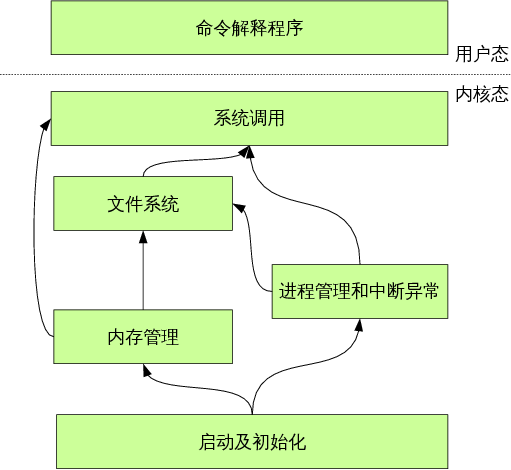
\includegraphics[height=8cm]{7-1}
  \caption{六个实验间的关系}\label{fig:7-1}
\end{figure}

\section{操作系统实验工具}

\subsection{交叉编译器}
首先,整个实验是建立在MIPS上的,通过之前的计算机组成等课程的学习我们知道,不同类型的CPU有不同的ISA。我们本地常使用的是Intel的X86指令集,
或AMD64(EMT64)等指令集。而我们的小操作系统的目标机是MIPS指令集的。但我们需要使用交叉编译器来完成编译过程。
我们的交叉编译器运行于x86平台上,但编译产生的二进制文件却是在mips平台上运行的。如图\ref{fig:0-2}
所示,编译器所运行的平台与其编译出来的程序的平台不同,因此叫做交叉编译器。

\begin{note}
严格意义上来说,所谓平台包含了两个概念:体系结构(Architecture)、操作系统(Operating System)。
一个体系结构上,可以运行多种不同的操作系统。而同一个操作系统,也可以在不同体系结构上运行。
举例来说,我们常说的 x86 Linux 平台实际上是 Intel x86 体系结构和Linux for x86操作系统的统称;
而x86 WinNT平台实际上是Intel x86体系结构和Windows NT for x86 操作系统的简称。
\end{note}

交叉编译器通常用于解决目标平台因性能不足等原因难以直接在其上开发的问题。举个例子,假如我们需要为一个500MHz的ARM开发程序,
因为其性能、工具、环境等原因,我们很难直接在这个ARM的板子上进行开发。因此,我们可以选择在一个性能强劲、工具齐全的x86 PC机上完成程序,
再通过交叉编译器编译为ARM指令集的程序。通过这样的方式,我们就能够轻松地为ARM开发程序了。

\begin{figure}[htbp]
  \centering
  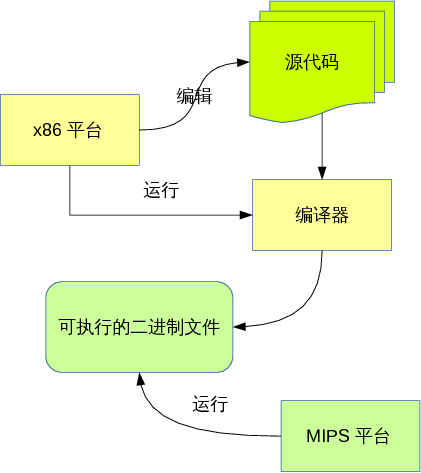
\includegraphics[height=8cm]{7-2}
  \caption{交叉编译}\label{fig:7-2}
\end{figure}

\subsection{Linux系统}
Unix是一个经典的操作系统。目前操作系统中的很多设计思想以及算法均是源自Unix的。
但Unix在商业化后,我们很难以相对廉价的方式直接接触Unix。目前相对较为完善的自由的Unix衍生版仅有FreeBSD等寥寥几个,
其上的软件生态环境等等十分有限。不过,幸运的是,Linux为我们提供了一个相对良好的接触Unix思想的机会。
Linux是一个自由的类Unix(Unix-like)系统,兼容POSIX标准,为我们的实验提供了一个良好的环境。
近些年Linux发展迅猛,其上的软件环境等也十分丰富,这一点相较于BSD家族来说要好很多。
我们实验中采用了GNU的工具,这一套工具主要是为Unix类系统编写的。同时,我们的小操作系统中有很多Unix风格的设计,
因此,采用Linux平台做实验更有利于大家理解实验中的很多内容。实验为大家提供的虚拟机上的环境是一个无图形界面的Ubuntu 12.04,
大家通过ssh远程连接到虚拟机上去做实验。通过命令行界面来进行全部的操作。很多同学以前没有太接触过这种操作方式,这一点需要大家慢慢熟悉。

\begin{note}
事实上,Linux仅仅是一个操作系统内核。一般一个完整的基于Linux的操作系统还包含GNU的各类工具软件,
图形环境,应用软件等等其他一系列的软件。但习惯上,将以Linux为内核的操作系统简称为Linux。
由于大家长期以来习惯在Linux内核上使用大量的GNU软件,所以,Richard Stallman认为将这类操作系统称为“GNU/Linux”更为恰当。
\end{note}

\section{实验环境配置}

\subsection{Linux操作系统}
由于所有的实验都是在Linux下完成的,所以需要Linux操作系统。我们选用设计上更为用户友好的Ubuntu系统。
有两种可供参考的安装方式,一是通过虚拟机来安装Linux系统,二是直接安装Linux系统。这里考虑到大部分同学对于Linux不同熟悉,
我们介绍虚拟机安装的方法。

首先,我们需要下载操作系统的镜像。为了下载速度考虑,我们选择从中国科学与技术大学的镜像站\url{http://mirrors.ustc.edu.cn/}上下载。
点击该页面右侧的\textbf{获取安装镜像},出现如图\ref{fig:get-ubuntu-image}所示的界面,版本选择与实验环境一致的12.04。

\begin{figure}[htbp]
  \centering
  \includegraphics[width=15cm]{get-ubuntu-image}
  \caption{获取安装镜像}\label{fig:get-ubuntu-image}
\end{figure}

接下来,我们下载虚拟机软件。虚拟机相当于一台虚拟的机器,虚拟机上的操作就好像是在操作另一台机器,对本机不会造成影响,
是相对安全的一种体验Linux的方案。这里我们选择采用VirtualBox虚拟机。可以去官网\url{https://www.virtualbox.org/wiki/Downloads}下载,
也可以去百度上自行寻找国内的较快的下载地址。当然,你也可以选择其他的虚拟机软件,如VMware(性能更佳,但是是专有软件,你懂得),具体操作相仿。
但Virtualbox是自由软件,所以出于版权方面的考虑,这里以VirtualBox为例。

安装VirtualBox(相信安装这种小事一定难不住你)后,打开它,看到如图\ref{fig:virtualbox-startup}所示的界面。

\begin{figure}[htbp]
  \centering
  \includegraphics[width=10cm]{virtualbox-startup}
  \caption{VirtualBox虚拟机界面}\label{fig:virtualbox-startup}
\end{figure}

点击\textbf{新建},出现如图\ref{fig:virtualbox-dialog1}所示的对话框。类型选择\textbf{Linux},版本选择\textbf{Ubuntu(64bit)}
(这里如果你下载的时候选择的是i386版本则选择\textbf{Ubuntu(32bit)})。点击\textbf{下一步},内存选择\textbf{1024MB}。
下一步,选择\textbf{现在创建虚拟硬盘},后面的设置如无特殊需求不必改动,一直下一步即可。直到选择磁盘大小处,建议选择\textbf{20GB},
同时选定一个至少有20GB空间的的位置放置磁盘镜像文件。

\begin{figure}[htbp]
  \centering
  \includegraphics[height=8cm]{virtualbox-dialog1}
  \caption{新建虚拟机}\label{fig:virtualbox-dialog1}
\end{figure}

之后选中我们刚才建立的虚拟机,点\textbf{设置},\textbf{存储},点选\textbf{光盘加号形状图标},\textbf{添加虚拟光驱},
如图\ref{fig:virtualbox-dialog2}然后\textbf{选择磁盘},选中之前下载好的Ubuntu的ISO文件。
      
\begin{figure}[htbp]
  \centering
  \includegraphics[width=10cm]{virtualbox-dialog2}
  \caption{选择启动镜像}\label{fig:virtualbox-dialog2}
\end{figure}

选中虚拟机,点击\textbf{启动},弹出虚拟机画面,启动后进入Ubuntu的安装界面(见图\ref{fig:ubuntu-install1})。
左侧可以选择语言,这里我们选择\textbf{English},并点击\textbf{Install Ubuntu}。
(当然,按理说选择中文也是没问题的,但这里为了避免任何不必要的麻烦,我们选择了英文)。

\begin{figure}[htbp]
  \centering
  \includegraphics[width=10cm]{ubuntu-install1}
  \caption{选择启动镜像}\label{fig:ubuntu-install1}
\end{figure}

之后由于我们没有改镜像源等设置,为了安装速度考虑,不要选择\textbf{Download updates while installing}。以免Ubuntu
从缓慢的官方服务器下载更新。\textbf{Install this third-party software}选项与我们实验无关,你可以自行选择是否勾选。
下一步选择\textbf{Erase disk and install Ubuntu}。由于我们是在虚拟机上安装,且使用了新建的虚拟磁盘,所以自然可以大胆
地让Ubuntu清空整个磁盘并安装。下一步一般不需要做改动,点击\textbf{Install Now}就好。之后输入密码,等待安装结束就好。

\begin{figure}[htbp]
  \centering
  \includegraphics[width=10cm]{ubuntu-install2}
  \caption{Ubuntu安装中新建用户的界面}\label{fig:ubuntu-install2} 
\end{figure}

安装结束后点击\textbf{Restart}重启。重启时注意,安装镜像关闭时一般会提示你取出光盘并按回车键。
光盘镜像正常情况下会被自动弹出。
一般来说,你需要做的仅仅是按下回车键并等待重启。
这里注意,有时候由于种种原因它不会输出这句提示,遇到这种情况就需要发动你的第六感了:)感觉系统不再动了以后敲一个回车就好。

重启完成后登入Ubuntu界面,接下来我们安装增强功能。点击虚拟机的\textbf{设备},然后选择\textbf{安装增强功能}。
之后会Ubuntu会选择弹出对话框询问是否自动运行,如图\ref{fig:ubuntu-install3}所示。点击\textbf{Run}后会
弹出对话框要求输入密码,输入密码后会启动一个命令行,开始执行安装脚本,看到\textbf{Press Return to close this window}
后按回车键结束安装。手动重启虚拟机,重启后虚拟机的分辨率会变成相对正常的状态,说明增强功能已经成功安装。

\begin{figure}[htbp]
  \centering
  \includegraphics[width=8cm]{ubuntu-install3}
  \caption{Ubuntu安装中新建用户的界面}\label{fig:ubuntu-install3} 
\end{figure}

至此,一个Ubuntu环境就搭建完成了。你可以在上面学习并熟悉Linux的相关指令,并编写我们的实验代码。

\begin{exercise}
安装一个Linux环境,并尝试学会使用ls、cat、cd、cp、mv这五条指令
\end{exercise}

\subsection{安装交叉编译器}
交叉编译器的下载可以访问\url{http://ftp.sunet.se/pub/Linux/distributions/eldk/4.1/mips-linux-x86/iso/}
到其中下载\textbf{mips-2007-01-21.iso}文件。这里下载网速较慢,建议大家下载完一份后相互拷贝,
一般课程中心也会提供相应的文件。

在Ubuntu下,按住Ctrl+Alt+t快捷键,可以打开一个终端,我们在终端中

\begin{minted}[linenos]{bash}
# 建立一个用于挂载ISO镜像的目录
sudo mkdir /mnt/mipsiso
# 挂载iso文件
sudo mount -o loop mips-2007-01-21.iso /mnt/mipsiso
# 切换到/mnt/mipsiso文件夹中
cd /mnt/mipsiso
# 安装32位运行库(仅在64位系统上需要执行此步骤)
sudo apt-get install ia32-libs
# 运行安装脚本
sudo ./install -d /opt/eldk
\end{minted}

执行完上面的指令后,检查/opt/eldk/usr/bin下是否有以mips\_4KC开头的一系列工具。
打开命令行,尝试运行其中的gcc,如果看到如下输出,则说明一切OK~

\begin{minted}[linenos]{bash}
# 注意,此时需要位于/opt/eldk/usr/bin目录下
$ ./mips_4KC-gcc
Reading specs from /opt/eldk/usr/bin/../lib/gcc/mips-linux/4.0.0/specs
Target: mips-linux
Configured with: /opt/eldk/build/mips-2007-01-21/work/usr/src/denx/
BUILD/crosstool-0.35/build/gcc-4.0.0-glibc-2.3.5-eldk/mips-linux/
gcc-4.0.0/configure --target=mips-linux --host=i686-host_pc-linux-gnu 
--prefix=/var/tmp/eldk.PyrfxY/usr/crosstool/gcc-4.0.0-glibc-2.3.5-eldk
/mips-linux --with-headers=/var/tmp/eldk.PyrfxY/usr/crosstool/gcc-4.0.
0-glibc-2.3.5-eldk/mips-linux/mips-linux/include --with-local-prefix=
/var/tmp/eldk.PyrfxY/usr/crosstool/gcc-4.0.0-glibc-2.3.5-eldk/
mips-linux/mips-linux --disable-nls --enable-threads=posix 
--enable-symvers=gnu --enable-languages=c,c++ --enable-shared 
--enable-c99 --enable-long-long --enable-__cxa_atexit
Thread model: posix
gcc version 4.0.0 (DENX ELDK 4.1 4.0.0)
\end{minted}

\subsection{安装仿真器}
由于实验的操作系统内核是运行在mips体系结构上的,而我们平常使用的是基于x86体系结构的PC,
所以需要使用仿真器来仿真一个mips体系结构的环境,来让我们的操作系统内核运行。在这个实验中我们使用的是 gxemul 仿真器。

我们需要从\url{http://gxemul.sourceforge.net/src/}下载gxemul-0.4.6.tar.gz。
这里需要注意,一定要下载0.4系列的gxemul,而不是最新的0.6系列,以免发生和实验提供的文件发生不兼容的现象。
调出终端,切换到gxemul-0.4.6.tar.gz所在目录,执行以下指令

\begin{minted}[linenos]{bash}
# 解压gxemul-0.4.6.tar.gz
tar -zxvf gxemul-0.4.6.tar.gz
# 进入gxemul文件夹
cd gxemul-0.4.6
# 配置并编译安装
./configure
make
sudo make install
sudo cp gxemul /usr/local/bin
\end{minted}

在命令行中执行gxemul指令,看到如下输出则说明gxemul安装正确。

\begin{minted}[linenos]{bash}
$ gxemul
GXemul 0.4.6    Copyright (C) 2003-2007  Anders Gavare
Read the source code and/or documentation for other Copyright messages.

usage: gxemul [machine, other, and general options] [file [...]]
   or  gxemul [general options] @configfile
   or  gxemul [userland, other, and general options] file [args ...]

Run  gxemul -h  for help on command line options.

No filename given. Aborting.
\end{minted}

\begin{exercise}
安装交叉编译器及gxemul,并确认其正常运行。
\end{exercise}

\section{实验思考}

\begin{thinking}
思考以下几条指令有何作用?
  \begin{itemize}
    \item ls -l
    \item mv test1.c test2.c
    \item cp test1.c test2.c
    \item cd ..
  \end{itemize}
\end{thinking}
我们的整个实验环境全部是运行于Linux基础上的,且所提供的虚拟机是没有安装图形界面的,需要通过ssh远程连接访问。
实验的所有操作全部在命令行下完成。因此,在开始实验前,你需要掌握最基本的一些命令,以保证你可以\textbf{在命令行下生存}

\begin{thinking}
思考grep指令的用法,例如如何查找项目中所有的宏?如何查找指定的函数名?
\end{thinking}
grep指令可以在文件中\textbf{匹配特定的文本}。支持递归匹配(即查找当前目录及子目录下所有文件)、正则表达式等一系列有用的功能。
当你需要在整个项目目录中查找某个函数名、变量名等等的时候,grep将是你手头一个强有力的工具。
这里给一个提示,grep的-a、-i、-r三个选项使用率较高,可以着重了解一下。

\begin{thinking}
思考gcc的-Werror和-Wall两个参数在项目开发中的意义。
\end{thinking}
编译器警告很多时候可以帮你发现一些代码上的错误。善用编译器警告可以大大加快你调试的进度。

\end{appendix}
\end{document}
